% ========================================= TEMPLATE INFO ========================================
%
% Author:       P4ntomime
% Version:      1.0.0
% Last updated: 2024-02-18
% Brief:        A LaTeX template for summaries. See README.md for more information.
% 
% ================================================================================================
\documentclass[8pt, a4paper, twoside]{extarticle}
% Font size:    8pt
% Paper size:   A4
% style:        twoside (needed, so odd and even pages have different margins)
% orientation:  portrait. (use 'landscape' for landscape orientation)


% ========================================= DOCUMENT INFO =========================================
\def\title{Wahrscheinlichkeit und Statistik}           					% title
\def\shorttitle{WrStat} 												% short title (displayed as PDF title)
\def\dozent{Prof. Dr. Andreas Müller}         							% lecturer
\def\semester{HS 2026}     												% semester
\def\author{Simone Stitz}        										% author(s)
\def\repo{https://gitlab.com/sstitz/wahrscheinlichkeit-und-statistik}   % repository link
\def\version{3.0.\today}    											% version
\def\pagelimit{20}           											% page limit -> causes pages after limit to be red
\def\titleoption{normal}   												% options: compact, normal
\def\enableToC{true}

% ================================= PACKAGES, SETUP AND COMMANDS ==================================
% =========================================== PACKAGES ============================================
\usepackage[utf8]{inputenc}         % input encoding: UTF-8
\usepackage[T1]{fontenc}            % font encoding: T1
\usepackage{textcomp}               % additional symbols
\usepackage{times}                  % times new roman font
\usepackage[main=ngerman]{babel}    % set main language to german


\usepackage{multicol}               % provides multicols environment
\usepackage{geometry}               % set page layout


\usepackage{enumitem}               % list customization
\usepackage{outlines}               % easy nested lists
\usepackage{tabularx}               % some nicer tables with X columns
\usepackage{hhline}                 % double lines in tables
\usepackage{booktabs}               % thick and thin lines in tables


\usepackage{amsmath}                % math symbols
\usepackage{amssymb}                % more math symbols
\usepackage{mathtools}              % more math tools needed for pmatrix modification
\usepackage{mhsetup}                % needed to modify pmatrix environment
\usepackage{txfonts}                % Times math font
\usepackage[squaren]{SIunits}       % SI-units
\usepackage{bm}                     % bold math symbols
\usepackage{trfsigns}               % needed for "Laplace" symbol (Korrespondenz)
\usepackage{mathrsfs}               % needed for Fourier transform "F"


\usepackage{graphicx}               % include graphics
\usepackage{graphbox}               % needed for aligning images in multicol environment
\usepackage{scalerel}               % scale any objects
\usepackage{anyfontsize}            % set any font size
\usepackage{xcolor}                 % needed for colors


\usepackage{tcolorbox}              % colored boxes
\usepackage[outline]{contour}       % contour for text (used in custom underline command)
\usepackage[normalem]{ulem}         % custom underline (used in custom underline command)


\usepackage{tikz}                   % needed for TikZ drawings


% \usepackage{listings}               % for nicer code display
% to use nodes inside listing see: https://texample.net/tikz/examples/tikz-listings/


\usepackage{hyperref}               % clickable links
\usepackage{qrcode}                 % QR code generation (also clickable)


\usepackage{ifthen}                 % if-then-else commands
\usepackage{calc}                   % simple arithmetic in LaTeX commands


\usepackage{draftwatermark}         % watermark on pages after a certain limit
\usepackage{fancyhdr}               % custom header and footer
\usepackage[explicit]{titlesec}     % custom section titles


\usepackage{datetime2}              % custom date format for versioning


% ========================================== BASIC SETUP ==========================================

% --------------------------------------- DOCUMENT SETTINGS ---------------------------------------
\hypersetup{hidelinks,
% set pdf metadata
            pdfauthor={\author},
            pdftitle={\shorttitle},
            pdfsubject={\title\ \semester},
            pdfkeywords={Gahn go lerne!!}}

% set style for URLs
\urlstyle{same} % sets url font to the same as the preceeding text

% set page layout
\geometry{left=3mm, 
          right=3mm, 
          top=3mm, 
          bottom=6mm, 
          headheight=0mm, 
          headsep=0mm, 
          footskip=4mm}

\setlength{\columnsep}{1.5mm}       % distance between columns
\setlength{\columnseprule}{0.1pt}   % thickness of column separation line
\setlength{\parindent}{0pt}         % no paragraph indentation

\setcounter{tocdepth}{2}            % only display sections and subsections in toc
% \setcounter{secnumdepth}{0}       % uncomment to disable section numbering

\DeclareMathSizes{8}{8}{6}{5}       % set math font sizes for 8pt document


% --------------------------------------- COLOR DEFINITIONS ---------------------------------------
\definecolor{sectioncolor}{HTML}{9665cb}
\definecolor{subsectioncolor}{HTML}{b2a6d8}
\definecolor{sectextcol}{HTML}{fcf9f9}
\definecolor{subsectextcol}{HTML}{000000}

\definecolor{backcolour}{HTML}{f5f5f0} % background color for highlighted text

% TODO: define color palette
% color palette: https://colorkit.co/color-palette-generator/FF8552-9e22bd-404E7C-C32E15-225A28/
\definecolor{green}{HTML}{1af430}
\definecolor{red}{HTML}{f90d09}
\definecolor{blue}{HTML}{093ce5}
\definecolor{orange}{HTML}{f7730e}
\definecolor{violet}{HTML}{a516c9}

% colors for listings (code)
% \definecolor{commentcolour}{HTML}{404E7C}
% \definecolor{keywordcolour}{HTML}{225A28}
% \definecolor{stringcolour}{HTML}{9e22bd}
% \definecolor{numbercolour}{HTML}{808080}


% ----------------------------------- LIST AND TABULAR SETTINGS -----------------------------------
\setlist[enumerate]{%
    labelindent=0pt,                                % no indentation for labels
    labelwidth = \widthof{\ref{enum-\EnumitemId}},  % set label width to widest label
    label=\bfseries\arabic*.,                       % label style bold arabic numerals (1., 2., ...)
    itemindent=1ex,                                 % separation between label and item text
    leftmargin=!,                                   % automatically calculate left margin
    after=\label{enum-\EnumitemId}}                 % set label for referencing in labelwidth

\setlist[itemize]{leftmargin=1.5em}                 % left margin for itemize: 1.5em
\setlist{nosep}                                     % no vertical spacing between list items

\renewcommand{\arraystretch}{1}                     % stretch table rows

\setcounter{MaxMatrixCols}{32}                      % increase max columns in matrix environments

% ----------------------------------------- TIKZ SETTINGS -----------------------------------------
\usetikzlibrary{arrows}
\usetikzlibrary{arrows.meta}
\usetikzlibrary{bending}
\usetikzlibrary{decorations.pathreplacing}
\usetikzlibrary{angles}
\usetikzlibrary{tikzmark}
\usetikzlibrary{petri}
\usetikzlibrary{positioning}
\usetikzlibrary{shapes}
\usetikzlibrary{calc}


% ------------------------------------ OTHER PACKAGE SETTINGS -------------------------------------

% define and set new date style for versioning as YYYYMMDD
\DTMnewdatestyle{vnumdate}{%
    \renewcommand{\DTMdisplaydate}[4]{\number##1\DTMtwodigits{##2}\DTMtwodigits{##3}}%
    \renewcommand{\DTMDisplaydate}{\DTMdisplaydate}%
}
\DTMsetdatestyle{vnumdate}


% setup for ulem and contour packages
\renewcommand{\ULdepth}{1.75pt} % set underline depth
\contourlength{0.7pt}           % set contour length


% ====================================== SETUP AND COMMANDS =======================================

\ExplSyntaxOn
% custom underline command for exclusions on lowercase letters such as g, j, p, q, y
\newrobustcmd{\myul}[1]{%
    \if_mode_math:
        \text{%
            \uline{\phantom{$#1$}}%
            \llap{\contour{white}{$#1$}}%
        }
    \else:
        \uline{\phantom{#1}}%
        \llap{\contour{white}{#1}}%
    \fi:
}

\renewrobustcmd{\underline}[1]{%
    \if_mode_math:
        \text{%
            \uline{\phantom{$#1$}}%
            \llap{\contour{white}{$#1$}}%
        }
    \else:
        \uline{\phantom{#1}}%
        \llap{\contour{white}{#1}}%
    \fi:
}
\ExplSyntaxOff


% setup header and footer
\pagestyle{fancy}
\fancyhf{}                          % clear all header and footer fields
\renewcommand{\headrulewidth}{0pt}  % remove header rule
\renewcommand{\footrulewidth}{0pt}  % remove footer rule
\fancyfoot[C]{\thepage}             % page number in center of footer


% --------------------------------------- TITLE FORMATTING ----------------------------------------

% section formatting
\titleformat{\section}
            % {\fontsize{9}{8}\selectfont\bfseries}
            {\Large\bfseries}
            {}
            {0mm}
            {\tikz{
                \node[fill=sectioncolor,            % fill color:       sectioncolor
                      text=sectextcol,              % text color:       sectextcol
                      text width=\columnwidth-4pt,  % text width:       columnwidth - 2x padding
                      text depth=0pt,               % text depth:       0pt (needed so text stays vertically centered)
                      minimum height=5mm,           % minimum height:   5mm
                      inner sep=2pt,                % inner padding:    2pt
                      align=left]                   % text alignment:   left
                      {\thesection\ #1};}}

\titleformat{numberless, name=\section}
            % {\fontsize{9}{8}\selectfont\bfseries}
            {\Large\bfseries}
            {}
            {0mm}
            {\tikz{
                \node[fill=sectioncolor,            % fill color:       sectioncolor
                      text=sectextcol,              % text color:       sectextcol
                      text width=\columnwidth-4pt,  % text width:       columnwidth - 2x padding
                      text depth=0pt,               % text depth:       0pt (needed so text stays vertically centered)
                      minimum height=5mm,           % minimum height:   5mm
                      inner sep=2pt,                % inner padding:    2pt
                      align=left]                   % text alignment:   left
                      {#1};}}

\titlespacing{\section}
             {0mm}
             {.2ex}
             {.2ex}


% subsection formatting
\titleformat{\subsection}
            {\large\bfseries}
            {}
            {0mm}
            {\phantomsection\tikz{
                \node[fill=subsectioncolor,         % fill color:       subsectioncolor 
                      text=subsectextcol,           % text color:       subsectextcol 
                      text width=\columnwidth-4pt,  % text width:       columnwidth - 2x padding 
                      text depth=0pt,               % text depth:       0pt (needed so text stays vertically centered)
                      minimum height=5mm,           % minimum height:   5mm 
                      inner sep=2pt,                % inner padding:    2pt 
                      align=left]                   % text alignment:   left
                      {\thesubsection\ #1};}}

\titleformat{numberless, name=\subsection}
            {\large\bfseries}
            {}
            {0mm}
            {\phantomsection\tikz{
                \node[fill=subsectioncolor,         % fill color:       subsectioncolor 
                      text=subsectextcol,           % text color:       subsectextcol 
                      text width=\columnwidth-4pt,  % text width:       columnwidth - 2x padding 
                      minimum height=5mm,           % minimum height:   5mm 
                      inner sep=2pt,                % inner padding:    2pt 
                      align=left]                   % text alignment:   left
                      {#1};}}

\titlespacing{\subsection}
             {0mm}
             {1ex}
             {.2ex}


% subsubsection formatting
\titleformat{\subsubsection}
            {\large\bfseries}
            {\myul{\thesubsubsection\ }}
            {0mm}
            {\phantomsection{}\myul{#1}}

\titlespacing{\subsubsection}
             {0mm}
             {1ex}
             {1ex}


% paragraph formatting
\titleformat{\paragraph}[runin]
            {\semilarge\bfseries}
            {}
            {0mm}
            {#1\normalfont :\;}

\titlespacing{\paragraph}
             {0mm}
             {0ex}
             {0.1ex}


% new alias for paragraph '\para' (shorter than \paragraph)
\let\para\paragraph%

% custom command for examples
\newcommand{\example}[1]{\subsubsection*{Beispiel: #1}}


% ----------------------------------- CUSTOM TABULAR SPECIFIERS -----------------------------------

% centered fixed width column type
\newcolumntype{P}[1]{>{\centering\arraybackslash}p{#1}}

 % centered variable width column type
\newcolumntype{C}{>{\centering\arraybackslash}X}

% centered math column type
\newcolumntype{M}{>{$}c<{$}}


% inline tikz node for later referencing
\newcommand{\tikznode}[2]{% from https://tex.stackexchange.com/a/402466/121799
	\ifmmode%
	\tikz[remember picture,baseline= (#1.base),inner sep=0pt] \node(#1){$#2$};
	\else
	\tikz[remember picture,baseline= (#1.base),inner sep=0pt] \node(#1){#2};
	\fi}


% custom inline tcolorbox
\newtcbox{\mybox}
            [1]
            [backcolour]
            {on line,
            arc=0pt,
            outer arc=0pt,
            colback=#1,
            colframe=#1,
            boxsep=0pt,
            left=1pt,
            right=1pt,
            top=1pt,
            bottom=1pt,
            boxrule=0pt}


\makeatletter

% ------------------------------- SECTIONING COMMANDS CUSTOMIZATION -------------------------------

% section: add optional argument to command for script page numbers
\let\old@sec\section%
\RenewDocumentCommand{\section}{somg}{%
    \IfBooleanTF{#1}{
        \IfNoValueTF{#2}{
            \IfNoValueTF{#4}{
                \old@sec*{#3}
            }{
                \old@sec*{#3 {\small(S. #4)}}
            }
        }{
            \IfNoValueTF{#4}{
                \old@sec*[#2]{#3}
            }{
                \old@sec*[#2]{#3 {\small(S. #4)}}
            }
        }%
    }{
        \IfNoValueTF{#2}{
            \IfNoValueTF{#4}{
                \old@sec{#3}
            }{
                \old@sec{#3 {\small(S. #4)}}
            }
        }{
            \IfNoValueTF{#4}{
                \old@sec[#2]{#3}
            }{
                \old@sec[#2]{#3 {\small(S. #4)}}
            }
        }%
    }
}


% subsection: add optional argument to command for script page numbers
\let\old@subsec\subsection%
\RenewDocumentCommand{\subsection}{somg}{%
    \IfBooleanTF{#1}{
        \IfNoValueTF{#2}{
            \IfNoValueTF{#4}{
                \old@subsec*{#3}
            }{
                \old@subsec*{#3 {\small(S. #4)}}
            }
        }{
            \IfNoValueTF{#4}{
                \old@subsec*[#2]{#3}
            }{
                \old@subsec*[#2]{#3 {\small(S. #4)}}
            }
        }%
    }{
        \IfNoValueTF{#2}{
            \IfNoValueTF{#4}{
                \old@subsec{#3}
            }{
                \old@subsec{#3 {\small(S. #4)}}
            }
        }{
            \IfNoValueTF{#4}{
                \old@subsec[#2]{#3}
            }{
                \old@subsec[#2]{#3 {\small(S. #4)}}
            }
        }%
    }
}


% subsubsection: add optional argument to command for script page numbers
\let\old@subsubsec\subsubsection%
\RenewDocumentCommand{\subsubsection}{somg}{%
    \IfBooleanTF{#1}{
        \IfNoValueTF{#2}{
            \IfNoValueTF{#4}{
                \old@subsubsec*{#3}
            }{
                \old@subsubsec*{#3 {\small(S. #4)}}
            }
        }{
            \IfNoValueTF{#4}{
                \old@subsubsec*[#2]{#3}
            }{
                \old@subsubsec*[#2]{#3 {\small(S. #4)}}
            }
        }%
    }{
        \IfNoValueTF{#2}{
            \IfNoValueTF{#4}{
                \old@subsubsec{#3}
            }{
                \old@subsubsec{#3 {\small(S. #4)}}
            }
        }{
            \IfNoValueTF{#4}{
                \old@subsubsec[#2]{#3}
            }{
                \old@subsubsec[#2]{#3 {\small(S. #4)}}
            }
        }%
    }
}


% custom text rightarrow to match tikz arrows
\renewrobustcmd{\textrightarrow}{%
    \raisebox{0.2ex}{%
        \tikz[line width=0.11ex, >={Stealth[length=1.1ex, inset=0.2ex]}]{%
            \draw (0,-0.13ex) to (0.55em, -0.13ex);%
            \draw (0, 0.13ex) to (0.55em,  0.13ex);%
            \draw[line width=0pt, ->] (0.8em,0) to (0.9em,0);%
        }%
    }%
}%

% custom text leftrightarrow to match tikz arrows
\newrobustcmd{\textlrarrow}{%
    \raisebox{0.2ex}{%
        \tikz[line width=0.11ex, >={Stealth[length=1.1ex, inset=0.2ex]}]{%
            \draw (0.35em,-0.13ex) to (0.9em, -0.13ex);%
            \draw (0.35em, 0.13ex) to (0.9em,  0.13ex);%
            \draw[line width=0pt, ->] (1.15em,0) to (1.25em,0);%
            \draw[line width=0pt, <-] (0,0) to (0.1em,0);%
        }%
    }%
}%


% renews the pmatrix environment to use \lgroup and \rgroup instead of \left( and \right)
\renewenvironment{pmatrix}{%
    \left\lgroup%
    \matrix@check\pmatrix\env@matrix%
}{
    \endmatrix\right\rgroup%
}

% renews the pmatrix* environment to use \lgroup and \rgroup instead of \left( and \right)
\MHInternalSyntaxOn%
\renewenvironment{pmatrix*}[1][c]
  {\left\lgroup\MT_matrix_begin:N #1}
  {\MT_matrix_end:\right\rgroup}
\MHInternalSyntaxOff%


% new environment for centered tabulars
\NewDocumentEnvironment{ctabular}{m}
                        {\center\tabular{#1}}
                        {\endtabular\endcenter}


% custom command for size matched colored brackets
\newcommand{\bbr}[2]{\colorlet{saved}{.}\color{#1}\left(\color{saved}#2\color{#1}\right)\color{saved}}


% custom command for differential operator d
\newcommand{\diff}{\ensuremath{\mathop{} \! \mathrm{d}}}

% custom command for underset limes operator
\newcommand{\limes}[1]{\ensuremath{\underset{#1}{\lim}}}

% custom command for absolute value
\newcommand{\abs}[1]{\ensuremath{\left|#1\right|}}

% custom command for variance
\newcommand{\var}{\ensuremath{\mathrm{var}}}

% custom command for covariance
\newcommand{\cov}{\ensuremath{\mathrm{cov}}}

% custom command for binomial distribution
\newcommand{\Bi}{\ensuremath{\mathrm{Bi}}}


% shortcuts for colored text
\newcommand{\cgn}[1]{{\color{green}#1}}
\newcommand{\crd}[1]{{\color{red}#1}}
\newcommand{\cbl}[1]{{\color{blue}#1}}
\newcommand{\cor}[1]{{\color{orange}#1}}
\newcommand{\cvt}[1]{{\color{violet}#1}}



% bullet command for items in tables
\newcommand{\tabitem}{~~\llap{\textbullet}~~}


% customizes watermark and page color after a certain page limit
% colors all pages after the specified limit red
% source: https://stackoverflow.com/questions/2720534/force-a-maximum-number-of-pages-in-latex 
\newcounter{page@count}
\setcounter{page@count}{0}
\gdef\maxpages{\pagelimit}
\ifx\latex@outputpage\@undefined\relax% ChkTeX 21
    \global\let\latex@outputpage\@outputpage% ChkTeX 21
\fi%
\gdef\@outputpage{% ChkTeX 21
    \addtocounter{page@count}{1}%
    \ifnum\value{page@count}>\maxpages\relax%
        % change page background to red and add watermark
        \SetWatermarkText{\pagelimit\ Seiten Limit erreicht!}%
        \SetWatermarkScale{0.35}%
        \pagecolor{red}
        \latex@outputpage%
    \else%
        \SetWatermarkText{}%
        \latex@outputpage%
    \fi%
}


% remove title from table of contents, needed for layout
\renewcommand{\tableofcontents}{%
    \@starttoc{toc}
}


% scale super- and subscript -- not used currently, instead resized math font
% \catcode`_=\active% chktex 41 --> suppress ChkTeX warning
% \catcode`^=\active% chktex 41
% \newcommand_[1]{\ensuremath{\sb{\mathrm{\scaleobj{0.7}{#1}}}}}
% \newcommand^[1]{\ensuremath{\sp{\mathrm{\scaleobj{0.7}{#1}}}}}


\makeatother


% new environment for layout --> automatically adjusts to landscape or portrait
\ExplSyntaxOn
\NewDocumentEnvironment{layout}{}{
    \dim_compare:nNnT{\paperwidth}<{\paperheight}
    {
        % PORTRAIT LAYOUT
        \str_case:en{\str_lowercase:f\titleoption}
        {
            {compact}
            {
                \str_if_eq:eeTF {\str_lowercase:f\enableToC}{true}
                {
                    \begin{minipage}[t]{0.1\columnwidth} % Elo-like formatting
                        \raisebox{-.3\columnwidth}{\qrcode[level=L, 
                                version=0,
                                height=0.9\columnwidth]{\repo}}\\[1mm]
                        \normalfont\footnotesize V \version{}
                        \smallskip
                    \end{minipage}\hfill
                    \begin{minipage}[t]{0.89\columnwidth}
                        \raggedright%
                        \normalfont\Huge\bfseries\title{}\\[1mm]
                        \normalfont\Large\semester\ --\ \dozent{}\\
                        \large Autoren:\ \author{}\\[1mm]
                        \myul{\url{\repo}}
                    \end{minipage}\par
                    \section*{\contentsname}
                    \group_begin:
                    \setlength{\columnsep}{5mm}
                    \begin{multicols}{2}
                        \tableofcontents%
                    \end{multicols}
                    \group_end:
                    \vfill
                    \newpage
                    \begin{multicols*}{2}
                    \raggedcolumns%
                }
                {
                    \begin{multicols*}{2}
                    \raggedcolumns%
                    \begin{minipage}[t]{0.2\columnwidth} % MathFML-like formatting
                        \vspace{-0.225\columnwidth}
                        \qrcode[level=L, 
                                version=0,
                                height=0.9\columnwidth]{\repo}\\[1mm]
                        \normalfont\footnotesize V \version{}
                        \smallskip
                    \end{minipage}\hfill
                    \begin{minipage}[t]{0.79\columnwidth}
                        \raggedright%
                        \normalfont\Huge\bfseries\title{}\\[1mm]
                        \normalfont\Large\semester\ --\ \dozent{}\\
                        \large Autoren:\ \author{}\\[1mm]
                        \normalsize\myul{\url{\repo}}
                    \end{minipage}\par
                }
            }
            {normal}
            {
                \hfill\null\vspace{1cm}
                \begin{center}
                    \normalfont\fontsize{35}{32}\selectfont\bfseries\title{}\\[7.5mm]
                    \normalfont\huge\semester\ --\ \dozent{}\\
                    \Large Autoren:\\
                    \Large\author{}\\[2mm]
                    \large Version:\\
                    \large\version{}\\
                    \normalsize\myul{\url{\repo}}\\[2mm]
                    \qrcode[level=L, 
                            version=0,
                            height=2cm]{\repo}
                \end{center}
                \vfill
                \thispagestyle{empty}
                \str_if_eq:eeT {\str_lowercase:f\enableToC}{true}
                {
                    \section*{\contentsname}
                    \group_begin:
                    \setlength{\columnsep}{5mm}
                    \begin{multicols}{2}
                        \tableofcontents%
                    \end{multicols}
                    \group_end:
                    \vfill
                }
                \newpage
                \begin{multicols*}{2}
                \raggedcolumns%
            }
        }
    }
    
    \dim_compare:nNnT{\paperwidth}>{\paperheight}
    {
        % LANDSCAPE LAYOUT
        \begin{multicols*}{3}
        \raggedcolumns%            
        \begin{minipage}[t]{0.18\columnwidth}
            \vspace{-0.225\columnwidth}
            \qrcode[level=L, 
                    version=0,
                    height=0.9\columnwidth]{\repo}\\[1mm]
            \normalfont\footnotesize V \version{}
            \smallskip
        \end{minipage}\hfill
        \begin{minipage}[t]{0.81\columnwidth}
            \raggedright%
            \normalfont\Huge\bfseries\title{}\\
            \normalfont\Large\semester\ --\ \dozent{}\\
            \large Autoren:\ \author{}\\
            \normalsize\myul{\url{\repo}}
        \end{minipage}\par % \par needed or else there is an underfull hbox warning
        \str_if_eq:eeT {\str_lowercase:f\enableToC}{true}
        {
            \section*{\contentsname}
            \resizebox{\columnwidth}{!}{%
                \begin{minipage}[t]{1.2\columnwidth}
                    \begin{multicols}{2}
                        \tableofcontents%
                    \end{multicols}
                \end{minipage}
            }\par
        }
    }%
}
{\end{multicols*}}
\ExplSyntaxOff

% ---------------------------------------- LISTINGS SETUP -----------------------------------------

% % hack to fix asterisk in lstlisting
% \makeatletter
% \lst@CCPutMacro%
%     \lst@ProcessOther{"2A}{% ChkTeX 18
%          {\raisebox{0.125pt}{*}}}
%     \@empty\z@\@empty% ChkTeX 21
% \makeatother


% % inline lst tikz node for later referencing
% \newcommand{\lstnode}[2][0.5ex]{
% 	\tikz[overlay, remember picture, inner sep=0pt, yshift=#1, minimum width=0mm]\node(#2){};
% }


% custom inline listings with box around them
% \newcommand{\mylstbox}[2][columns=fullflexible]{
%     \mybox{
%         \lstinline[#1]{#2}}}
% \newcommand{\mytclstbox}[2][columns=fullflexible]{
%     \mybox{
%         \lstinline[basicstyle=\sffamily\footnotesize\color{#1}, columns=fullflexible]{#2}}}


% % renew command for lstinputlisting with less vertical spacing
% \renewcommand{\lstinputlisting}[2][]{
%     \begingroup
%     \vspace{-0.6\abovedisplayskip}
%     \lst@setcatcodes%
%     \lst@inputlisting[#1]{#2}
%     \vspace{-0.6\abovedisplayskip}
% }


% % listings style (code)
% \lstdefinestyle{mystyle}{
%     backgroundcolor=\color{backcolour},   
%     commentstyle=\color{commentcolour},
%     keywordstyle=\bfseries\color{keywordcolour},
%     numberstyle=\tiny\color{numbercolour},
%     stringstyle=\color{stringcolour},
%     basicstyle=\sffamily,
%     breakatwhitespace=false,
%     breaklines=true,
%     captionpos=b,
%     keepspaces=true,
%     numbers=left,
%     numbersep=2pt,
%     showspaces=false,
%     showstringspaces=false,
%     showtabs=false,
%     tabsize=4,
% 	xleftmargin=1em,
% 	language=Java,
%     extendedchars=true,
%     inputencoding=cp1252,
% 	columns=[l]fullflexible	% see: https://tex.stackexchange.com/questions/99416/latex-source-code-listing-with-less-space-between-characters or manual
% }


% % custom lstinline command with custom colors
% \def\purplst{\begingroup\color{violet}}
% \def\greenlst{\begingroup\color{green}}
% \def\redlst{\begingroup\color{red}}
% \def\ywlst{\begingroup\color{orange}}
% \def\bluelst{\begingroup\color{blue}}
% \def\endlstcol{\endgroup}


% % basic lstinline style without colors
% \lstdefinestyle{basestyle}{
%     backgroundcolor=\color{backcolour},
%     keywordstyle=\bfseries,
%     numberstyle=\tiny\color{numbercolour},
%     basicstyle=\sffamily\footnotesize,
%     breakatwhitespace=false,     
%     breaklines=true,
%     captionpos=b,
%     keepspaces=true,
%     numbers=none,
%     numbersep=2pt,
%     showspaces=false,
%     showstringspaces=false,
%     showtabs=false,
%     tabsize=4,
%     xleftmargin=0em,
%     language=Java,
%     columns=flexible,	% see: https://tex.stackexchange.com/questions/99416/latex-source-code-listing-with-less-space-between-characters or manual
% }


% \lstset{
%     style=mystyle,
%     morekeywords={final, override, enum, var, List, Set, Map, String, Object},
%     moredelim=[il][\textcolor{orange}]{¦¦},
%     moredelim=[is][\textcolor{orange}]{&&}{&&},
%     moredelim=[is][\textcolor{violet}]{@}{@},
% }



% =========================================== DOCUMENT ============================================
\begin{document}
    \begin{layout}
        \section{Kombinatorik}

\subsection{Zählregeln}

\begin{minipage}[t]{0.48\columnwidth}
	\begin{center}
		\myul{\textbf{Disjunkte Vereinigung}}

		\vspace{0.2cm}

		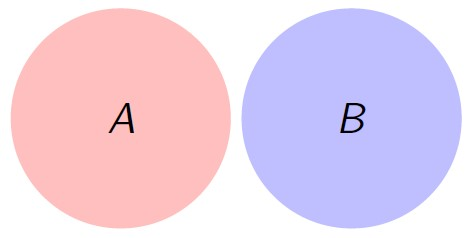
\includegraphics[height=2cm]{images/disjunkte_vereinigung.jpg}
		$$\lvert \crd{A} \cup \cbl{B} \rvert = | \crd{A} | + | \cbl{B} | $$
	\end{center}
\end{minipage}
\hfill
\begin{minipage}[t]{0.48\columnwidth}
	\begin{center}
		\myul{\textbf{Schnittmengen}}

		\vspace{0.2cm}

		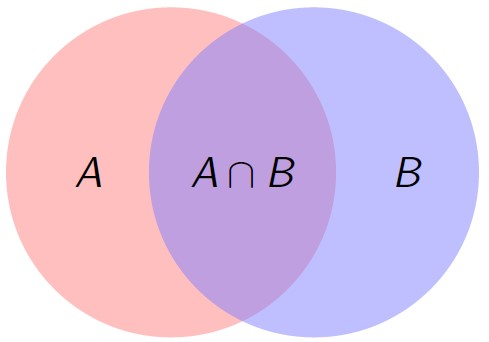
\includegraphics[height=2cm]{images/schnittmenge.jpg}
		$$ | \crd{A} \cup \cbl{B} | = | \crd{A} | + | \cbl{B} | - | \crd{A} \cap \cbl{B} | $$
	\end{center}
\end{minipage}

\vspace{0.2cm}
$$ | A \cup B \cup C | = |A| + |B| + |C| - |A \cap B| - |A \cap C| - |B \cap C| + |A \cap B \cap C| $$


\vspace{0.1cm}


\begin{minipage}[t]{0.48\columnwidth}
	\begin{center}
		\myul{\textbf{Paare = Produkt}}

		\vspace{0.2cm}

		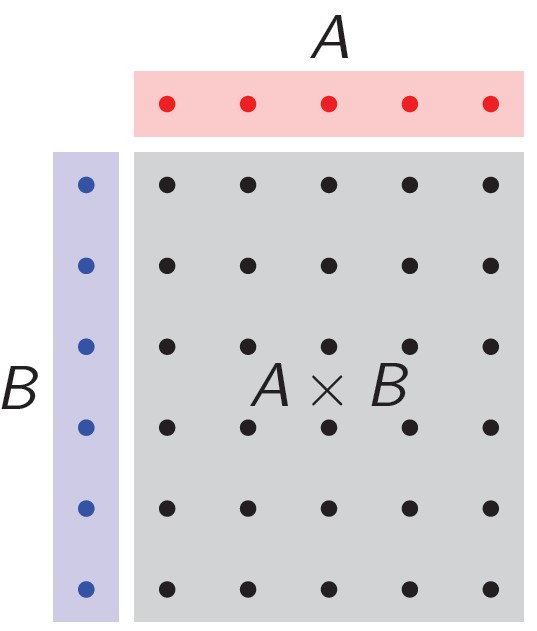
\includegraphics[width=0.7\columnwidth]{images/paare_produkt.jpg}
		$$ | \crd{A} \times \cbl{B} | = | \crd{A} | \cdot | \cbl{B} | $$	
	\end{center}
\end{minipage}
\hfill
\begin{minipage}[t]{0.48\columnwidth}
	\begin{center}
		\myul{\textbf{Produktregel}}
	\end{center}

	Für-jeden-gibt-es-Regel

	\vspace{0.2cm}

	\crd{Wichtigste Regel in der Kombinatorik} 

	\vspace{0.2cm}

	Wenn es für jede von $n$ Wahl-möglichkeiten $m$ mögliche weitere Wahlmöglichkeiten gibt, 
	dann gibt es insgesamt $n \cdot m$ Möglichkeiten 
\end{minipage}


\subsection{Anordnungsproblem / Reihefolge (Permutation)}

\textbf{Auf wie viele Arten kann man $\bm{n}$ Objekte (auf $\bm{n}$ Plätzen) anordnen?} \\
\textrightarrow\ Reihenfolge relevant, keine Wiederholungen
$$ \boxed{ \text{\#} \; \text{Möglichkeiten} = P_n = n! }$$


\subsection{Perlenkette (Variation)}
\textbf{Auf wie viele Arten kann man $\bm{k}$ mal unter $\bm{n}$ verschiedenen Objekte auswählen?}

\vspace{0.1cm}
\textbf{Auf wieviele Arten kann man eine Perlenkette der Länge $\bm{k}$ aus $\bm{n}$ Farben von Perlen herstellen?} \\
\textrightarrow\ Reihenfolge egal, Wiederholungen erlaubt; 'Ziehen mit zurücklegen'
$$\boxed{ \text{\#} \; \text{Möglichkeiten} = V_{n,k} = n^k } $$ 


\subsection{Auswahlproblem (Kombination)}

\textbf{Auf wieviele Arten kann man $\bm{k}$ Objekte aus $\bm{n}$ auswählen? (Lottoproblem)} \\
\textrightarrow\ Reihenfolge egal, keine Wiederholungen; 'Ziehen ohne zurücklegen'

$$\boxed{ \text{\#} \; \text{Möglichkeiten} = C_k^n = \frac{n!}{k! \, (n-k)!} = 
\begin{pmatrix} n \\ k \end{pmatrix} } $$ 

Taschenrechner: \texttt{COMB($n, \, k$)}


\subsection{Tipps und Tricks zu Kombinatorik}
\begin{itemize}
	\item Aufgabe in oben beschriebene Teilprobleme aufteilen
	\item Teillösungen \textbf{multiplizieren}
	\item Pensare in modalità albero di decisioni (moltiplicazione fra decisioni)
\end{itemize}


\subsection{Erzeugende Funktion}

Für $a_k \in \mathbb{R}, \; k = 0, \, 1, \, ...$, heisst $f(z)$ die \textbf{erzeugende Funktion} der Koeffizienten $a_k$
$$ f(z) = \sum\limits_{k=0}^\infty a_k \, z^k $$

\textrightarrow\ Die Funktion $f(z)$ erzeugt die Koeffizienten $a_k$ eines Polynoms der Form
$$ a_0 \, z^0 + a_1 \, z^1 + a_2 \, z^2 + ... + a_k \, z^k $$ 


\subsubsection{Beispiele für erzeugende Funktionen}

\begin{itemize}
	\setlength\itemsep{0.75em}
	\item $f(z) = \cbl{1} + \cor{1} \, z$ ist erzeugende Funktion von $a_k = (\cbl{1}, \, \cor{1}, \,0, \,0, \, ...)$
	\item $a_k = (\cbl{1}, \, \cor{2}, \, \cgn{3}, \, \crd{4})$ \textrightarrow\  $f(z) = \cbl{1} + \cor{2} \, z + \cgn{3} \, z^2 + \crd{4} \, z^3$
	\item $f(z) = (1 + z)^n$ ist erzeugende Funktion der Binomialkoeffizienten $a_k = \begin{pmatrix} n\\k \end{pmatrix}$
\end{itemize}


\vfill\null
\columnbreak


\subsubsection*{Anwendung: Münzwechsel}

\textbf{Gegeben:} 3 Einfränkler, 4 Zweifränkler, 7 Fünfliber \\
\textbf{Gesucht:} Auf wieviele Arten kann man jeden möglichen Betrag $k$ damit zahlen?

\vspace{0.2cm}

\begin{tabular}{ll}
	$0-3$ Einfränkler:	& $f_1(z) = 1 + z^1 + z^2 + z^3$ \\	
	$0-4$ Zweifränkler: & $f_2(z) = 1 + \cbl{0} \, z^{\cor{1}} + \cbl{1} \, z^{\cor{2}} + \cbl{0} \, z^{\cor{3}} + \cbl{1} z^{\cor{4}} + \ldots + \cbl{1} \, z^{\cor{8}}$ \\	
	$0-7$ Fünfliber: 	& $f_5(z) =  1 + 1 \, z^5 + 1 \, z^{10} + \ldots + 1 \, z^{35} $ \\	
	Alle Werte: 		& $f_1(z) \cdot f_2(z) \cdot f_5(z)$
\end{tabular}

\vspace{0.2cm}

\textrightarrow\ $\text{\cbl{{\# Mögl. um Betrag zu erreichen}}} \; z^{\cor{\text{Betrag in CHF}} }$


		\section{Ereignis und Wahrscheinlichkeit}

\subsection{Experimente und Ereignisse}

\begin{minipage}{0.35\columnwidth}
	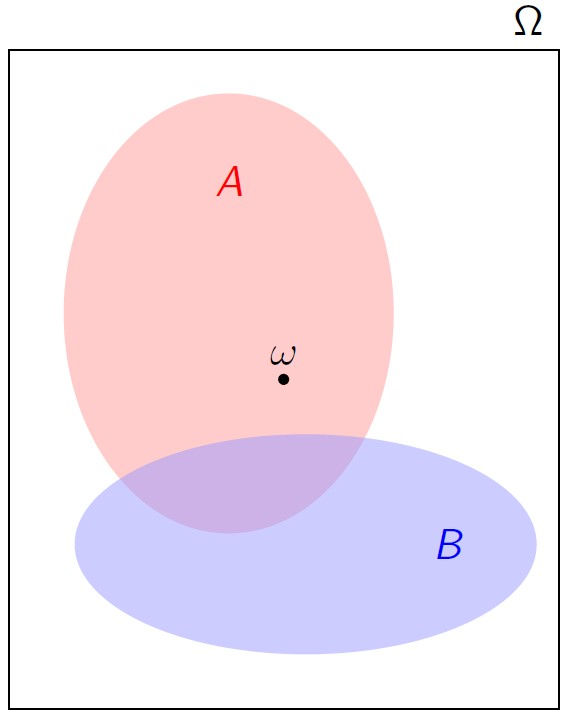
\includegraphics[width=\columnwidth]{images/ereignisse_begriffe.jpg}
\end{minipage}
\hfill
\begin{minipage}{0.64\columnwidth}
    \myul{\textbf{Elementarereignis $\bm{\omega}$}} \\
    Ausgang eines Experiments

\vspace{0.2cm}

\myul{\textbf{Experimente $\bm{\Omega}$}} \\
    Menge der möglichen Elementarereignisse $\omega$ 

\vspace{0.2cm}

\myul{\textbf{Ereignis}} \\
    Teilmenge von $\Omega$ \\
\crd{$A$} eingetreten \textlrarrow\ Versuchsausgang $\omega \in \crd{A}$ \\
\cbl{$B$} nicht eingetr. \textlrarrow\ Versuchsausgang $\omega \notin \cbl{B}$
\medbreak
\myul{\textbf{Insieme delle parti $\bm{\mathcal{P}(\Omega)}$}} \\
    $\mathcal{P}(\Omega)$ = insieme che contiene \textbf{tutti} i possibili sottoinsiemi di $\Omega$, cioè tutti i possibili eventi \\
    Esempio: se $\Omega = \{1,2,3\}$, allora $\mathcal{P}(\Omega)$ contiene $\emptyset,\ \{1\},\ \{2\},\ \{3\},\ \{1,2\},\ \{1,3\},\ \{2,3\},\ \{1,2,3\}$ \\
$$\abs{\mathcal{P}(\Omega)} = 2^{\abs{\Omega}} = 2^n$$
\end{minipage}

\subsection{Spezielle Ereignisse}

\subsubsection{Sicheres Ereignis}

Das Ereignis $A = \Omega$ tritt immer ein: $ A = \Omega \subset \Omega $


\subsubsection{Unmögliches Ereignis}

Das Ereignis $B = \emptyset$ tritt nie ein: $ B = \emptyset = \{ \} \subset \Omega $


\subsection{Ereignis-Algebra}

\renewcommand{\arraystretch}{1.4}
\begin{tabular}{|l | l | l |}
	\hline
				& $A \cup B$ 												& $A$ oder $B$ 							\\
	Ereignisse 	& $A \setminus B$ 											& $A$, aber nicht $B$ 					\\
				& $\Omega$ 													& Alles (Sicheres Ereignis) 			\\
	\hline
 				& $\emptyset = \Omega \setminus \Omega$ 					& Alles ohne alles (Unmögl. Ereignis) 	\\

	Folderungen & $\overline{A} = \Omega \setminus A$ 						& Alles ohne $A$						\\

				& $A \cup B = \overline{\overline{A} \cap \overline{B}}$ 	& De Morgan 							\\
	\hline
\end{tabular}
\renewcommand{\arraystretch}{1}


\subsubsection{Rechenregeln}

\begin{minipage}[t]{0.48\columnwidth}
	\renewcommand{\arraystretch}{1.2}
	\begin{tabular}{l}
		$A \cap (B \cup C) = ( A \cap B) \cup ( A \cap C )$ 	\\
		$A \cup (B \cap C) = (A \cup B) \cap ( A \cup C )$ 
	\end{tabular}
	\renewcommand{\arraystretch}{1}
\end{minipage}
\hfill
\begin{minipage}[t]{0.48\columnwidth}
	\renewcommand{\arraystretch}{1.2}
	\begin{tabular}{l}
		$\overline{A \cap B} = \overline{A} \cup \overline{B}$ \\
		$\overline{A \cup B} = \overline{A} \cap \overline{B}$ 
	\end{tabular}
	\renewcommand{\arraystretch}{1}
\end{minipage}


\subsection{Wahrscheinlichkeit}

Definition der Wahrscheinlichkeit:
$$ \boxed{ P(A) = \lim\limits_{\text{\# Versuche} \to \infty} \frac{\text{\# Versuche, bei denen $A$ eintritt}}{\text{\# Versuche}}  = \frac{\abs{A}}{\abs{\Omega}}} $$


\subsubsection{Axiome}

\begin{itemize}
	\item Wertebereich: $0 \leq P(A) \leq 1$ 
	\item Sicheres Ereignis: $P(\Omega) = 1$ 
	\item Disjunkte Vereinigung (keine Schnittmengen zwischen Ereignissen)\\
	$P(A_1 \cup A_2\cup ... \cup A_n \cup \dots) =  P(A_1) + P(A_2) + ... + P(A_n) + \dots$ 
\end{itemize}


\subsubsection{Eigenschaften}

\begin{itemize}
	\item Unmögliches Ereignis: $P(\emptyset) = 0$ 
	\item Komplementärereignis: $P(\overline{A}) = 1 - P(A)$
	\item Differenz: $P(A \setminus B) = P(A) - P(A \cap B)$
	\item Vereinigung: $P(A \cup B) = P(A) + P(B) \, \cor{- P(A \cap B)}$
	\item $P(A \cup B \cup C) = P(A) + P(B) + P(C) - P(A \cap B) - P(A \cap C) - P(B \cap C) + P(A \cap B \cap C)$
\end{itemize}


\subsection{Spezielle Arten von Experimenten}

\subsubsection{Laplace-Experimente}

Alle Versuchsausgänge haben die \textbf{gleiche Wahrscheinlichkeit} 
$$ \boxed{ P(A) = \frac{\text{Anzahl günstige Ausgänge}}{\text{Anzahl mögliche Ausgänge}} = \frac{\vert A \vert}{\vert \Omega \vert} }$$

Beispiele: (faire) Würfel, Karten ziehen, (faire) Münzen werfen


\subsubsection{Bernoulli-Experimente}

Genau \textbf{zwei }Versuchsausgänge mit Wahrscheinlichkeiten $p$ und $1-p$
$$ \boxed{ p = P(A), \qquad 1 - p = 1 - P(A) = P(\overline{A}) } $$


\subsection{Bedingte Wahrscheinlichkeit}

Die Bedingte Wahrscheinlichkeit ist die Wahrscheinlichkeit für \crd{$A$}, wenn \cbl{$B$} bereits eingetreten ist: 

\begin{minipage}{0.48\columnwidth}
	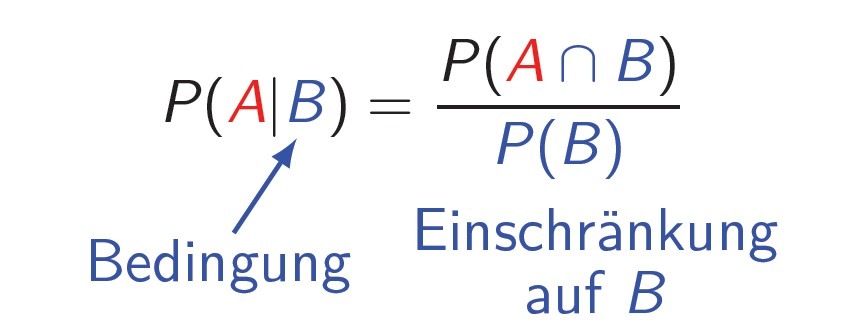
\includegraphics[width=\columnwidth]{images/bedingte_wahrscheinlichkeit.jpg}
\end{minipage}
\hfill
\begin{minipage}{0.48\columnwidth}
	\textbf{Im Allgemeinen ist}
	$$P(A|B) \neq P(B|A)$$
\end{minipage}


\subsubsection{Unabhängigkeit}

$A$ und $B$ heissen \textbf{unabhängig}, wenn
$$ \boxed{ P(A \cap B) = P(A) \cdot P(B) } \qquad \text{\color{red}Formula valida solo per \textbf{2} eventi!}$$ 

\begin{minipage}[t]{0.48\columnwidth}
	\begin{center}
		\myul{\textbf{Unabhängig}}

		\vspace{-0.5cm}

		$$ P(A|B) = P(A| \overline{B}) $$
		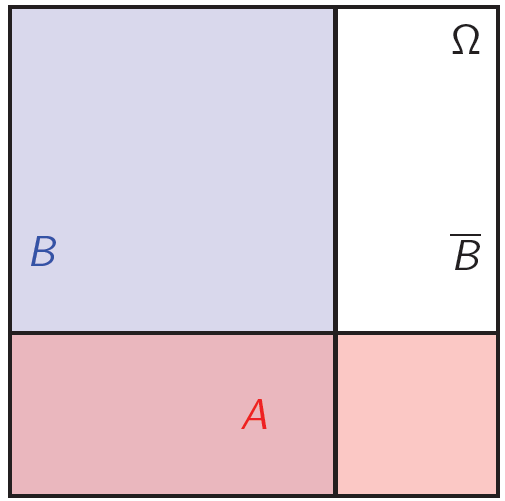
\includegraphics[width=0.6\columnwidth, align=t]{images/unabhaengig.png}
	\end{center}
\end{minipage}
\hfill
\begin{minipage}[t]{0.48\columnwidth}
	\begin{center}
		\myul{\textbf{Abhängig}}

		\vspace{-0.5cm}

		$$ P(A|B) < P(A| \overline{B}) $$
		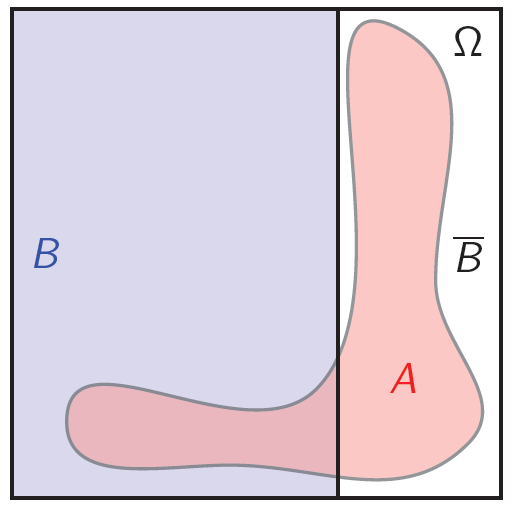
\includegraphics[width=0.6\columnwidth, align=t]{images/abhaengig.png}
	\end{center}
\end{minipage}


\subsection{Satz von Bayes}

Es gibt einen Zusammenhang zwischen den Wahrscheinlichkeiten, je nachdem welches Ereignis zuerst eintreten muss

$$ P(A \, | \, B) \cdot P(B) = P(A \cap B) = P(B \, | \, A) \cdot P(A) $$

\begin{minipage}{0.48\columnwidth}
	$$ \boxed{ P(A \, | \, B) = P(B \,| \, A) \frac{P(A)}{P(B)} } $$
\end{minipage}
\hfill
\begin{minipage}{0.48\columnwidth}
	$$ \boxed{ P(B \, | \, A) = P(A \,| \, B) \frac{P(B)}{P(A)} } $$ 
\end{minipage}

\vspace{0.2cm}
$$ \text{Wichtig: } P(A \, | \, B) = 1 - P( \overline{A} \, | \, B ) 
\text{ oder } 
P(A \vert \overline{B}) = 1 - P(\overline{A} \vert \overline{B})$$


\subsection{Totale Wahrscheinlichkeit} 

\textbf{Frage:} Wie gross ist die Wahrscheinlichtkeit, dass \crd{$A$} eintrifft? 
$$ \boxed{  P(\crd{A}) = P(\crd{A} \, | \, B_1) \cdot P(B_1) + ... + P(\crd{A} \, | \, B_n) \cdot P(B_n) } $$

wenn $B_i$ disjunkt und $\cup B_i = \Omega$ 


\example{Totale Wahrscheinlichkeit}

\begin{minipage}{0.4\columnwidth}
	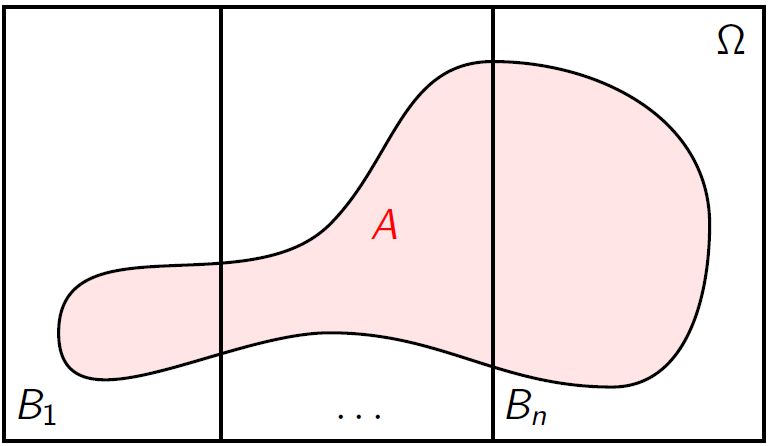
\includegraphics[width=\columnwidth]{images/totale_wahrscheinlichkeit.png}
\end{minipage}
\hfill
\begin{minipage}{0.56\columnwidth}
	\begin{tabular}{r c l }
		$P(Z \cap A)$ 	 	& $=$ 	& $P(Z|A) \cdot P(A)$ \\
		$ + P(Z \cap B)$ 	& $=$ 	& $P(Z|B) \cdot P(B)$ \\
		$ + P(Z \cap C)$ 	& $=$ 	& $P(Z|C) \cdot P(C)$ \\
	\hline
		$P(Z)$ 				& 		& 						\\
	\end{tabular}
\end{minipage}


		\section{Zufallsvariable und Erwartungswert}

\subsection[Zufallsvariable]{Zufallsvariable $\bm{X}$}

Die Zufallsvariable $X$ ist eine Funktion $X: \, \Omega \rightarrow \mathbb{R}$ , die einem Versuchsausgang $\omega$ einen Wert
$X(\omega)$ zuordnet. \\
\textrightarrow\ Ein Wert, der vom Ausgang eines Zufallsexperiments abhängt

\vspace{0.2cm}

Die Zufälligkeit liegt in dem Versuch, der das $\omega$ ermittelt. \\
Die Zuweisung des Wertes $X(\omega)$ ist \textbf{deterministisch}


\subsubsection{Diskrete Zufallsvariable}

\begin{minipage}[c]{0.58\columnwidth}
	\raggedright
	Eine Zufallsvariable heisst \textbf{diskret}, wenn sie nur \textbf{einzelne genau bestimmte Zahlenwerte}
	$x_1, \, x_2, \, x_3, \, ...$ annehmen kann
	
	\vspace{0.2cm}

	Beispiel: Würfel 
\end{minipage}
\hfill
\begin{minipage}[c]{0.4\columnwidth}
	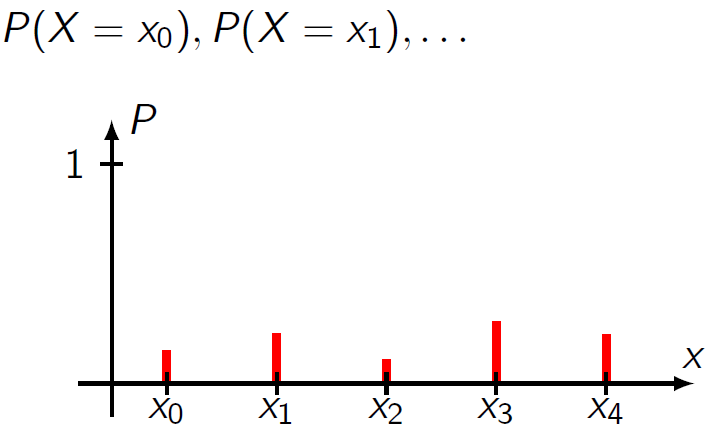
\includegraphics[width=\columnwidth]{images/wahrscheinlichkeit_diskrete_zufallsvariable.png}
\end{minipage}



\subsubsection{Stetige Zufallsvariable}


\begin{minipage}[c]{0.58\columnwidth}
	\raggedright
	Eine Zufallsvariable heisst \textbf{stetig}, wenn sie \textbf{beliebige Werte in einem Intervall} 
	annehmen kann (Wertemenge ist nicht diskret)

	\vspace{0.2cm}

	Beispiel: Messwerte
\end{minipage}
\hfill
\begin{minipage}[c]{0.4\columnwidth}
	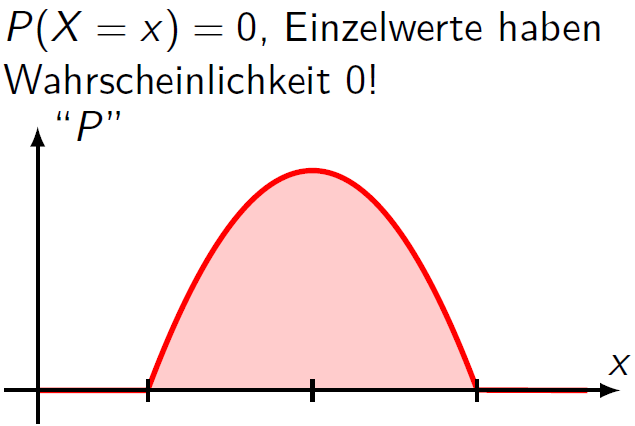
\includegraphics[width=\columnwidth]{images/wahrscheinlichkeit_stetige_zufallsvariable.png}
\end{minipage}




\subsubsection{Notation}

\myul{\textbf{Ereignisse}}

\vspace{0.1cm}

Die Zufallsvariable $X$ definiert neue Ereignisse \\
$A = \{ X \leq a  \} = \{ \omega \in \Omega | X(\omega) \leq a \}$ 

\vspace{0.2cm}

\myul{\textbf{Wahrscheinlichkeiten}}

\vspace{0.1cm}

$P(X = a) = P( \{ X \leq a  \}) = P( \{ \omega \in \Omega | X(\omega) \leq a \} )$ 



\subsection[Erwartungswert]{Erwartungswert  $\bm{E(X)}$} 

Ist $X$ eine Zufallsvariable, dann ist der Erwartungswert
$$  \boxed{ E(X) =\sum \text{Wert} \cdot \text{Wahrscheinlichkeit} } $$
$$ E(X) = \sum\limits_{\omega \in \Omega} X(\omega) \cdot P(\{ \omega \} ) = \sum\limits_{i=1}^k X(A_i) \cdot P(A_i)  $$ 
wobei $X$ konstant auf $A_i$ und $\cup \, A_i = \Omega$ sein muss.


\subsection{Empirischer Erwartungswert}

Der Empirische Erwartungswert entspricht einem \textbf{gewichteten Mittelwert} \\
\textrightarrow\ Notenberechnung

\begin{minipage}[c]{0.48\columnwidth}
	$$ P(X = x_i) = \frac{n_i}{n} $$
\end{minipage}
\hfill
\begin{minipage}[c]{0.48\columnwidth}
	\begin{tabular}{ll}
		$n_i$	& Gewichtung 		\\
		$n$ 	& Anzahl Messwerte
	\end{tabular}
\end{minipage}

\vspace{0.2cm}

$$ \boxed{ E(X) = \sum\limits_i X(i) \cdot P(X = x_i) \approx \sum\limits_i x_i \cdot \frac{n_i}{n} = \frac{x_1 n_1 + ... + x_k n_k}{n} } $$


\subsection{Rechenregeln Erwartungswert}

\textbf{Intuition:} Rechenregeln vom Differenzieren / Integrieren funktionieren auch für den Erwartungswert!


\subsubsection{Multiplikation mit Konstante}

\vspace{-0.2cm}
$$ \boxed{ E( \cor{\lambda} \, X) = \sum\limits_{\omega} \cor{\lambda} \, X(\omega) \cdot P(\omega) = \cor{\lambda} \cdot E(X) } $$


\subsubsection{Erwartungswert einer Konstanten $a$}

\vspace{-0.2cm}
$$ \boxed{ E(a) = a } $$


\subsubsection{Erwartungswert vom Erwartungswert}

\vspace{-0.2cm}
$$ \boxed{ E(E(X)) = E(X) } $$


\subsubsection{Summen}

\vspace{-0.2cm}
$$ \boxed{ E(X + Y) = E(X) + E(Y) } $$

\vspace{0.2cm}

\myul{\textbf{Herleitung}}

\vspace{0.1cm}

\begin{tabular}{ll}
	$E(X + Y)$	& $= \sum\limits_{\omega} \big( X(\omega) + Y(\omega)  \big) \cdot P(\omega)$ 										\\
				& $= \sum\limits_{\omega} X(\omega) \cdot P(\omega) + \sum\limits_{\omega} Y(\omega) \cdot P(\omega) = E(X) + E(Y)$
\end{tabular}
 

\subsubsection{Verbindung zur Wahrscheinlichkeit}

\textrightarrow\ Es gibt \textbf{nur zwei mögliche Versuchsausgänge}, man gewinnt oder man gewinnt nicht

\vspace{0.2cm}

Ist $ A \subset \Omega$ ein Ereignis, dann ist die \textbf{charakteristische Funktion} $\chi_A$ von $A$ eine Zufallsvariable 
$$ \chi_A: \, \Omega \rightarrow \mathbb{R}: \omega \mapsto \chi_A(\omega) =
\begin{cases} 1 & \omega \in A \\ 0 & \omega \notin A \end{cases} $$
Ihr Erwartungswert ist 
$$ \boxed{ E(\chi_A)= P(A) } $$

\vspace{0.2cm}

\myul{\textbf{Herleitung}}

\vspace{0.1cm}

$ E(\chi_A )=  \chi_A(A) \cdot P(A) + \chi_A(\overline{A}) \cdot P(\overline{A}) = 1 \cdot P(A) + 0 \cdot (1- P(A)) = P(A) $


\subsection{Unabhängigkeit}

$X$ und $Y$ sind unabhängig, wenn die Ereignisse $\{ X \leq x \} $ und $\{ Y \leq y \} $ unabhängig sind.

\vspace{0.2cm}

\begin{minipage}[c]{0.48\columnwidth}
	\begin{center}
		\crd{Bei Unabhängigkeit gilt:}
	\end{center}
	$$ \boxed{ E(XY) = E(X) \cdot E(Y) }$$
\end{minipage}
\hfill
\begin{minipage}[c]{0.48\columnwidth}
	\begin{tabular}{lcl}
		unabhängig		& $\Rightarrow$		& unkorreliert	\\
		unkorreliert 	& $\nRightarrow$ 	& unabhängig
	\end{tabular}
\end{minipage}


\subsection[Varianz]{Varianz $\bm{\var(X)}$}

Die Varianz misst die 'Streuung' einer Zufallsvariable und entspricht der mittleren quadratischen Abweichung vom Erwartungswert. \\
Die Formel gilt auch für empirische Daten (Messwerte)

\begin{minipage}[c]{0.4\columnwidth}
	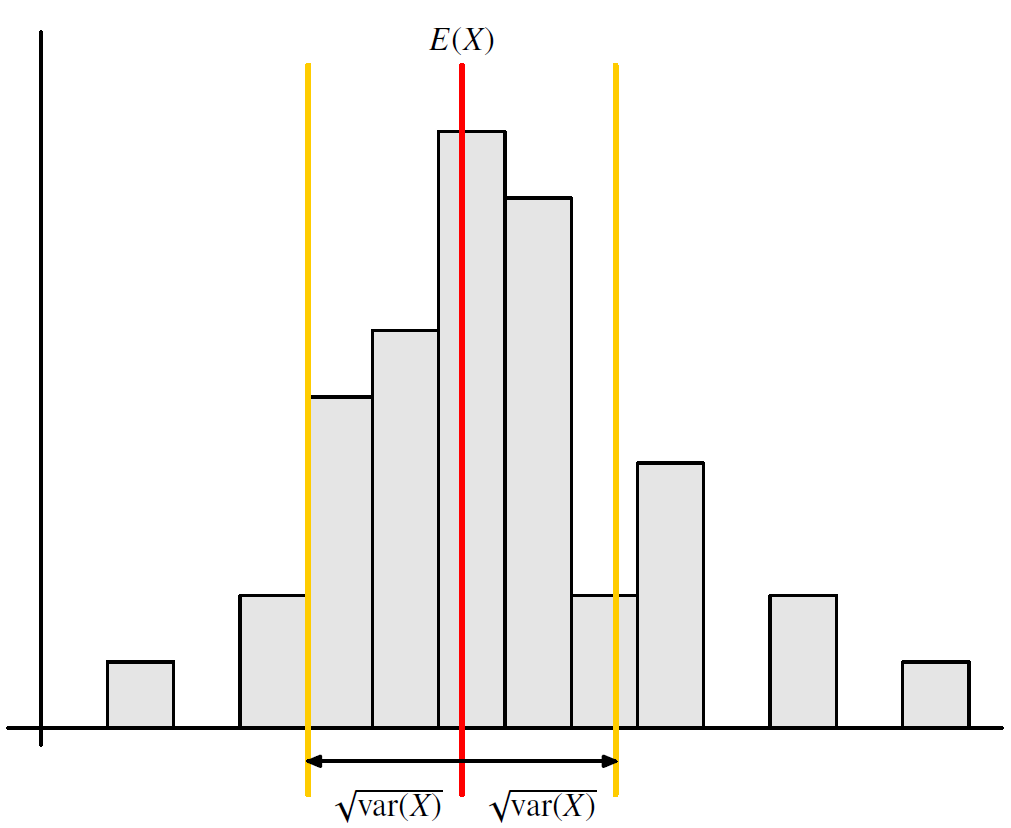
\includegraphics[width=\columnwidth]{images/varianz_darstellung.png}
\end{minipage}
\hfill
\begin{minipage}[c]{0.48\columnwidth}
	$$ \boxed{  \var(X) = E( \, (X - E(X))^2 \, ) }  $$
	$$ \boxed{  \var(X) = E(X^2) - E(X)^2 } $$
\end{minipage}


\subsubsection{Rechenregeln Varianz}

\crd{Für \textbf{unabhängige} Zufallsvariablen} $X$ und $Y$ gilt:

\vspace{0.2cm}

\begin{minipage}[c]{0.48\columnwidth}
	$$ \boxed{  \var(\lambda \, X) = \lambda^{\crd{2}} \var(X) } $$
\end{minipage}
\hfill
\begin{minipage}[c]{0.48\columnwidth}
	$$ \boxed{  \var(X + Y) = \var(X)+ \var(Y) } $$
\end{minipage}


\subsection[Kovazianz]{Kovazianz $\cov(X, \, Y)$}

Die Kovarianz ist ein Korrelationsmass für $X$ und $Y$ 
$$ \boxed{ \cov(X, \, Y) = E(XY) - E(X) \cdot E(Y) } $$


\subsection{Tschebyscheff-Ungleichung}

\textbf{Wahrscheinlichkeit, ausserhalb der Toleranz zu landen} \\
Ist $X$ eine Zufallsvariable mit Erwartungswert $\mu = E(X)$, dann gilt:

\vspace{0.2cm}

\begin{minipage}{0.48\columnwidth}
	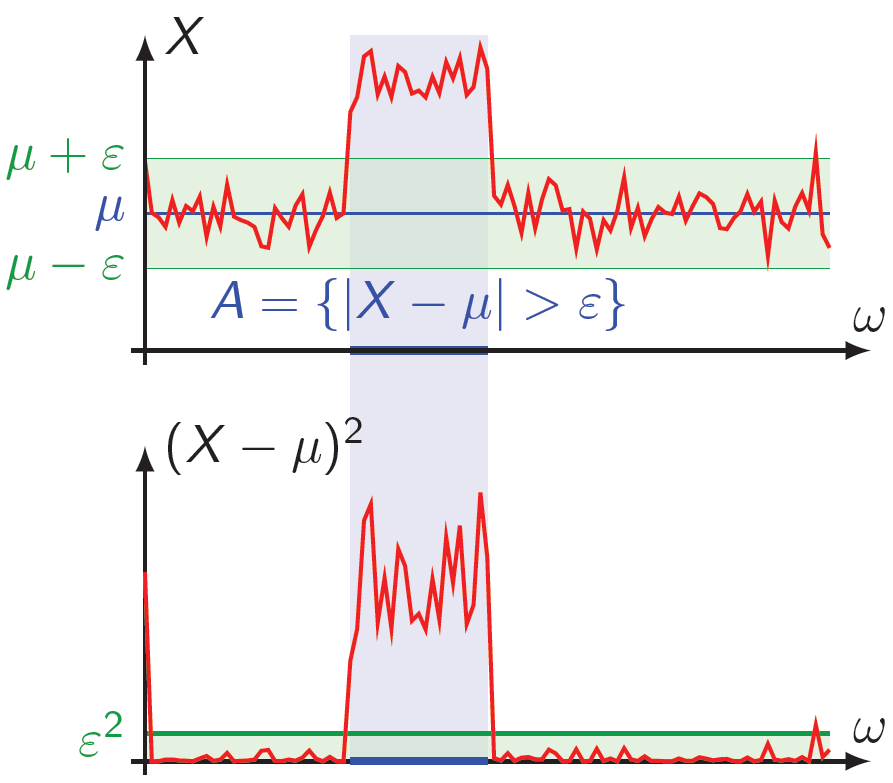
\includegraphics[width=\columnwidth]{images/tschebyscheff_ungleichung.png}
\end{minipage}
\hfill
\begin{minipage}{0.48\columnwidth}
	$$ \boxed{ P( | \crd{X} - \mu | > \varepsilon ) \leq \frac{\var(X)}{\varepsilon^2} = A } $$
	
	\vspace{0.2cm}

	\textrightarrow\ Wenn die Streubreite (Varianz) zunimmt, nimmt auch die Wahrscheinlichkeit zu, ausserhalb der 'Toleranz' zu landen
\end{minipage}


\subsection{Bernoulli: Genauigkeit des Mittelwertes}

\textbf{Abweichung des Mittelwerts vom Erwartungswert}

Gegeben: Zufallsvariable $X$ \\
Stichproben: $X_1, \, \ldots \, X_n$ Zufallsvariablen mit gleichem \\
Erwartungswert $\mu = E(X) = E(X_1) = \ldots = E(X_n)$ und gleicher \\
Varianz $\var(X) = \var(X_1) = \ldots = \var(X_n)$

\vspace{0.1cm}

$M_n = \frac{X_1 + \ldots + X_n}{n}$ \qquad $E(M_n) = E(X)$ \qquad $\var(M_n) = \frac{1}{n} \var(X)$
$$ \boxed{ P( | M_n - \mu | > \varepsilon ) \leq \frac{\var(X)}{ n \cdot \varepsilon^2} } $$

\textrightarrow\ Je mehr Messungen, desto unwahrscheinlicher eine grosse Abweichung des Mittelwerts vom Erwartungswert 


\subsection{Bernoulli: Gesetz der grossen Zahlen}

\textbf{Abweichung relative Häufigkeit von der Wahrscheinlichkeit} 

Ereignis: $A \subset \Omega$ \\
Experiment: $X = \chi_A$, Werte \{0,1\}, $P(A) = E(X)$, $\var(X) = P(A) - P(A)^2 = P(A)(1- P(A))$ 

\vspace{0.1cm}

Wiederholtes Experiment: $X_1, \, ..., \, X_n$, Stichprobe von $X$

\vspace{0.1cm}

Relative Häufigkeit: $h_n = \frac{X_1, \, ..., \, X_n}{n}$, $E(h_n) = P(A)$ \\
$\var(h_n) = \frac{1}{n} \var(X) = \frac{1}{n} P(A)(1-P(A))$ 

$$ \boxed{ P( | h_n - P(A) | > \varepsilon ) \leq \frac{P(A)(1-P(A))}{ n \cdot \varepsilon^2} \leq \frac{1}{4 \, n \, \varepsilon^2} } $$

\textrightarrow\ Je grösser die Anzahl Durchführungen $n$, desto kleiner die Wahrscheinlichkeit, dass die relative Häufigkeit 
stark von der Wahrscheilichkeit abweicht.


\subsection{Lineare Regression (Vorlage!)}

Ein Set von Messwerten $(x, \, y)$ soll mit einer \textbf{Geraden} $y = \cbl{a} \cdot x + \cbl{b}$ \textbf{approximiert} werden. 
Dabei sollen die Parameter $\cbl{a}$ und $\cbl{b}$ der Geraden so bestimmt werden, dass der \textbf{Fehler  $\var(Y-aX-b)$ \\ 
der Approximation minimal} wird.

\vspace{0.2cm}

\textrightarrow\ Entspricht 'Least Squares' Verfahren aus der Linearen Algebra 

$$  \boxed{ \cbl{a} = \frac{E(XY) - E(X) E(Y)}{E(X^2) - E(X)^2} = \frac{\cov(X,Y)}{\var(X)} } $$
$$  \boxed{ \cbl{b} = E(Y) - \cbl{a}  E(X) } $$


\subsubsection{Fehlerberechnung der Approximation}

\myul{\textbf{Fehler $\bm{Z}$}}
$$ \boxed{ Z = \var(Y) \Big( 1 - \frac{\cov(X,Y)^2}{\var(X) \, \var(Y)} \Big) = \var(Y)(1-r^2) } $$ 

\vspace{0.2cm}

\myul{\textbf{Regressionskoeffizient $r$}}
$$ \boxed{ r = \frac{\cov(X, Y)}{\sqrt{\var(X) \cdot \var(Y)}} } $$

\textrightarrow\ Der Fehler $Z$ wird klein, wenn $r^2$ nahe bei $1$ ist, also $r$ nahe bei $\pm 1$


\subsection{Nichtlineare Regression}

Mit einigen 'Umwandlungs-Tricks' können auch einige nichtlineare Funktionen linear gemacht werden und somit wieder
linear approximiert werden

\begin{center}
	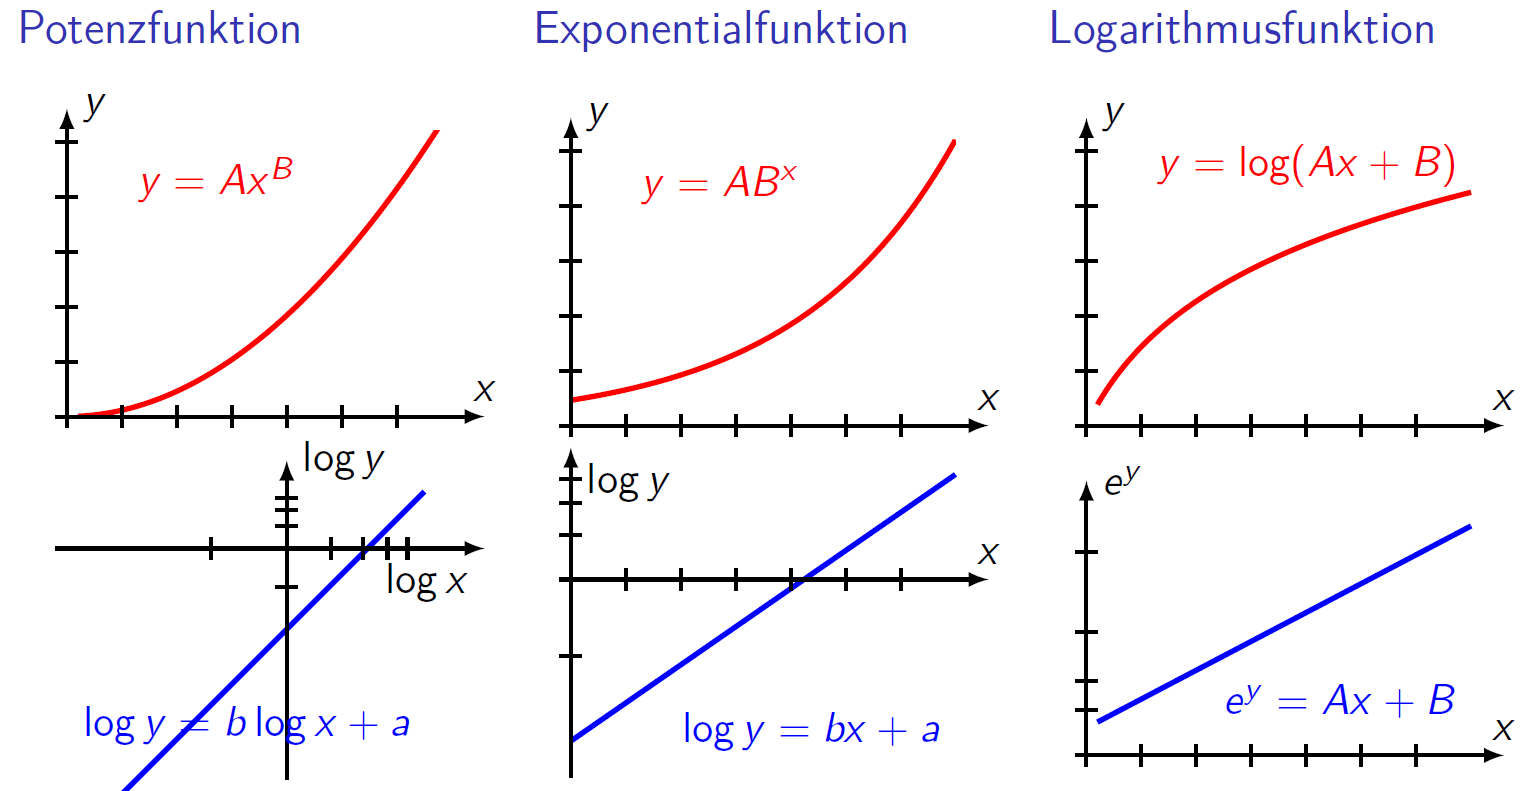
\includegraphics[width=0.8\columnwidth]{images/nichtlineare_regression.png}
\end{center}

\begin{tabular}{l c l}
	$y = Ax^B$			& \textrightarrow\	& $\log(y) = b \log(x) + \log(a)$ 	\\
						& \textrightarrow\ 	& $X = \log(x)$ ; $Y = \log(y)$ 	\\
	\\	
	$y = AB^x$ 			& \textrightarrow\ 	& $\log(y) = x (\log(B)) + \log(A)$ \\
						& \textrightarrow\ 	& $X = x$ ; $Y = \log(y)$ 			\\
	\\		
	$y = \log(Ax +B)$ 	& \textrightarrow\ 	& $e^y = Ax + B $					\\
						& \textrightarrow\ 	& $X = x$ ; $Y = e^y$
\end{tabular}


		\section{Wahrscheinlichkeitsverteilung}

\subsection{Kumulative Häufigkeitsverteilung}

\begin{minipage}{0.38\columnwidth}
	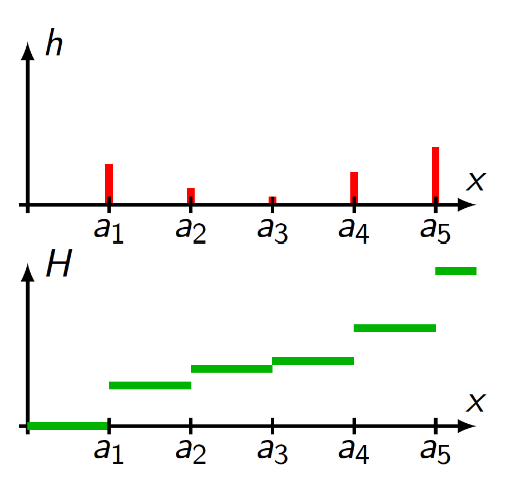
\includegraphics[width=\columnwidth]{images/kumulativeHaufigkeitsverteilung.png}
\end{minipage}
\hfill
\begin{minipage}{0.6\columnwidth}
	$$ H_j  = \sum\limits_{k=1}^j  h_k = | \{ x_i | x_i \leq a_j \} | $$
	$=$ Anzahl Merkmalsausprägungen 'links von $a_j$'
	
	\vspace{0.2cm}

	Allgemeiner:
	$$ H(x) = | \{ i | x_i \leq x \} | $$
	Stückweise konstant, Sprungstellen bei $a_j$ \\
	\textbf{Sprunghöhe} \crd{$h_j$}
\end{minipage}


\subsubsection{Relative Häufigkeit}

Maximum von $H(x)$ hängt von $n$ ab \textrightarrow relative Häufigkeit verwenden:

\begin{minipage}[c]{0.3\columnwidth}
	$$ f_j = \frac{1}{n} h_j $$
\end{minipage}
\hfill
\begin{minipage}[c]{0.3\columnwidth}
	$$ F_j = \frac{1}{n} H_j $$
\end{minipage}
\hfill
\begin{minipage}[c]{0.3\columnwidth}
	$$ F(x) = \frac{1}{n} H(x) $$
\end{minipage}


\subsection[Verteilungsfunktion]{Verteilungsfunktion $\bm{F}$}

\textbf{Definiton:}
Ist $X$ einer Zufallsvariable, so ist die Verteilungfunktion von $X$ definiert als
$$ \boxed{ F(x) = F_X(x) = P(X \leq x) } $$ 
Die Verteilungsfunktion beschreibt die \textbf{Wahrscheinlichkeit der Werte} einer Zufallsvariablen

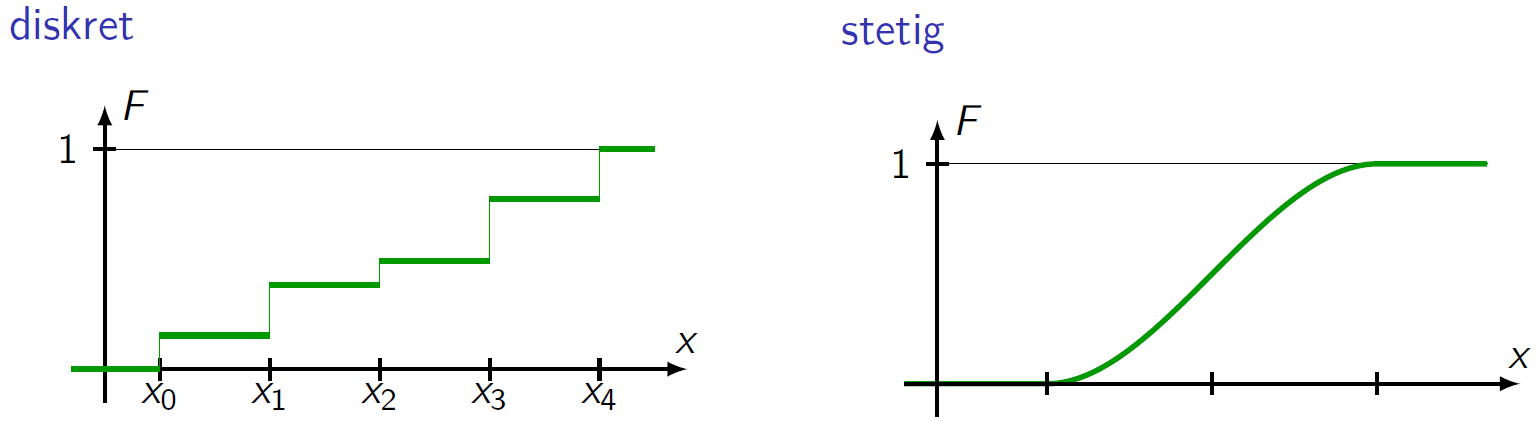
\includegraphics[width=0.9\columnwidth]{images/Verteilungsfunktion.png}


\subsubsection{Eigenschaften der Verteilungsfunktion}

\begin{itemize}
	\item $ F_X(x) $ ist monoton wachsend 
	\item $ 0 \leq F_X(x) \leq 1$ 
	\item $ \lim \limits_{x \to - \infty } F(x) = 0, \lim\limits_{x \to \infty} F(x) = 1 $ 
\end{itemize}

\vspace{0.2cm}

\begin{minipage}[t]{0.42\columnwidth}
	\begin{center}
		\myul{\textbf{Wahrscheinlichkeit für Intervall}}
		$$ \boxed{ P(a < X \leq b) = F_X(b) - F_X(a) } $$
	\end{center}
\end{minipage}
\hfill
\begin{minipage}[t]{0.55\columnwidth}
	\begin{center}
		\myul{\textbf{'Umkehrung'}}
		$$ \boxed{ P(X \leq x) = F(x) \text{ \textlrarrow\ } P( X > x) = 1 - F(x) } $$ 
	\end{center}
\end{minipage}


\subsubsection{Berechnung der Verteilungsfunktion}

Die Verteilungsfunktion $F(x) = P(X \leq x) $ ist eine Wahrscheinlichkeit 

\vspace{0.1cm}

\begin{enumerate}
	\item Fragen über $F(x)$ in Wahrscheinlichkeit von Ergebnissen übersetzen. 
	\item Rechenregeln für Wahrscheinlichkeit anwenden
	\item Wahrscheinlichkeit durch $F(x)$ ausdrücken, rückübersetzen 
\end{enumerate}


\example{Maximum zweier Zufallsvariablen}

\vspace{-0.2cm}

\begin{minipage}[c]{0.5\columnwidth}
	\textbf{Gegeben}\\
	Zwei unabh. Zufallsvariablen $X$ und $Y$ mit Verteilungsfunktion $F_X(x)$ und $F_Y(y)$
	\vspace{0.2cm}

	\textbf{Gesucht} \\
	Verteilungsfunktion $F_{\mathrm{max}(X,Y)}(x) = F_Z(z)$ 
\end{minipage}
\hfill
\begin{minipage}[c]{0.4\columnwidth}
	\begin{align*}
		F_Z(z)	&= P(Z  \leq z) 					\\
				&= P(\mathrm{max}(X,Y) \leq z) 		\\
				&= P(X \leq z \wedge  Y \leq z) 	\\
				&= P(X \leq z) \cdot P(Y \leq z) 	\\
		F_Z(z) 	&= F_X(z) \cdot F_Y(z)
		\end{align*} 
\end{minipage}


\subsubsection{Verteilungsfunktion des Maximums}

$X_1$ und $X_2$ sind zwei gleichverteilte Zufallsvariablen (z.B. Würfel)

\vspace{0.2cm}

Verteilungsfunktion von $F_{\mathrm{max}(X_1 ,X_2)}(x) = F_{X_1} (x_1)^2 = F_{X_2}(x_2)^2 $

\begin{center}
	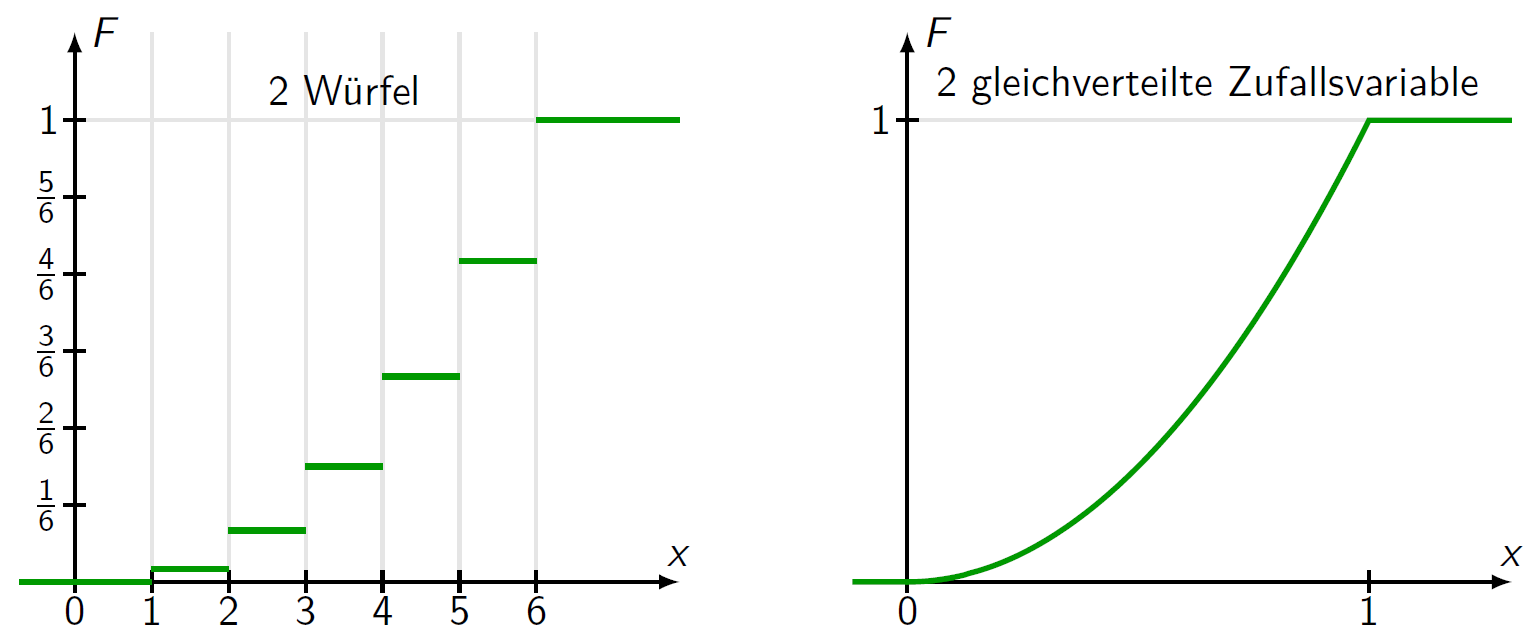
\includegraphics[width=0.8\columnwidth]{images/VerteilungsfunktionDesMaximums.png}
\end{center}


\subsection{Wichtige Werte in einem Diagramm}

\myul{\textbf{Mittelwert}}

\begin{minipage}[t]{0.48\columnwidth}
	$$ \boxed{ \crd{\overline{x}} = \frac{1}{n} \sum\limits_{i=1}^n x_i } $$
\end{minipage}
\hfill
\begin{minipage}[t]{0.48\columnwidth}
	$$ \boxed{ \text{minimiert: }  \sum\limits_{i=1}^n (x_i - \crd{\overline{x}})^2 } $$
\end{minipage}

\vspace{0.3cm}

\myul{\textbf{Gewichteter Mittelwert}}

\begin{minipage}[t]{0.48\columnwidth}
	$$ \boxed{ \crd{\overline{x}} = \frac{\sum\limits_{i=1}^n w_i \, x_i }{\sum\limits_{i=1}^n w_i } } $$
\end{minipage}
\hfill
\begin{minipage}[t]{0.48\columnwidth}
	$$ \boxed{ \text{minimiert: }  \sum\limits_{i=1}^n w_i \, (x_i - \crd{\overline{x}})^2 } $$
\end{minipage}

\vspace{0.3cm}

\begin{minipage}[t]{0.48\columnwidth}
	\raggedright
	\myul{\textbf{Median}}

	\vspace{0.1cm}

	Mittlerer Wert / 0.5-Quantil \\
	(Mittelwert der beiden mittleren Werte falls $n$ gerade ist) 

	\begin{center}
		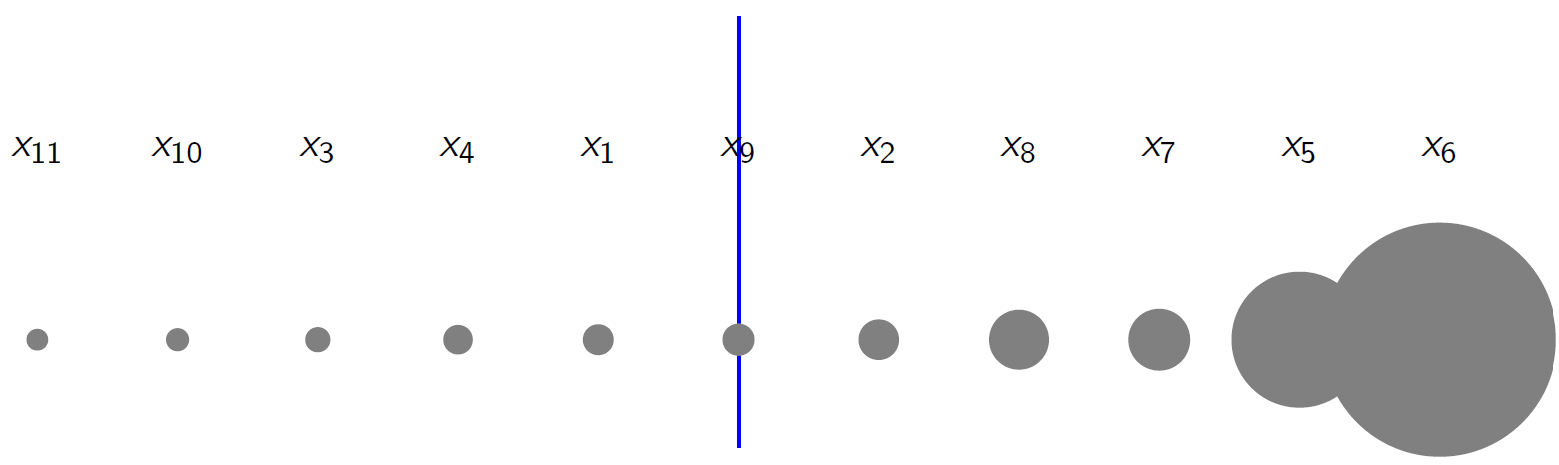
\includegraphics[width=0.9\columnwidth]{images/median.png}
	\end{center}
\end{minipage}
\hfill
\begin{minipage}[t]{0.48\columnwidth}
	\raggedright
	\myul{\textbf{Modus / Modalwert}}

	\vspace{0.1cm}

	Häufigster Wert

	\begin{center}
		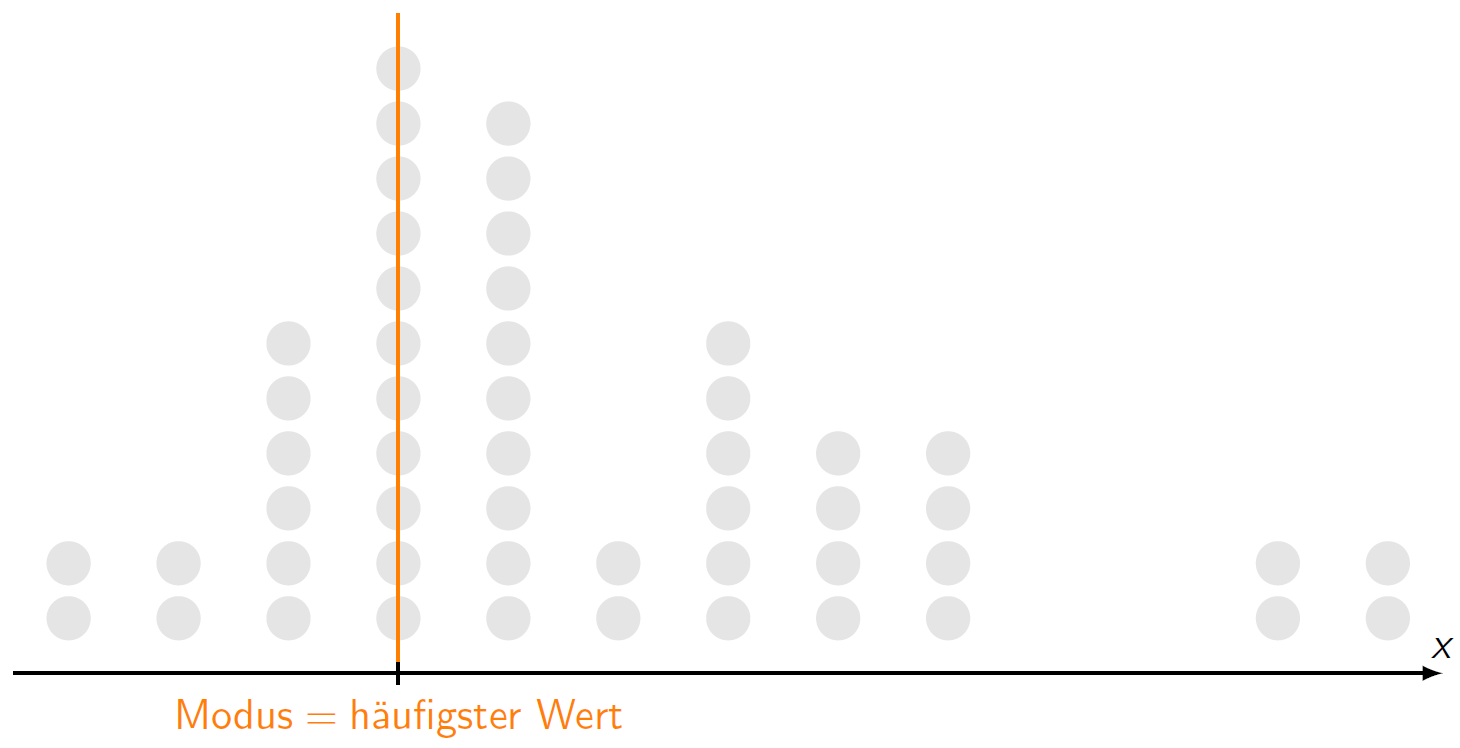
\includegraphics[width=0.85\columnwidth]{images/modus.png}
	\end{center}
\end{minipage}

\vspace{0.3cm}

\myul{\textbf{Spannweite $\bm{R}$ / Quartilabstand $\bm{Q}$}}

\begin{center}
	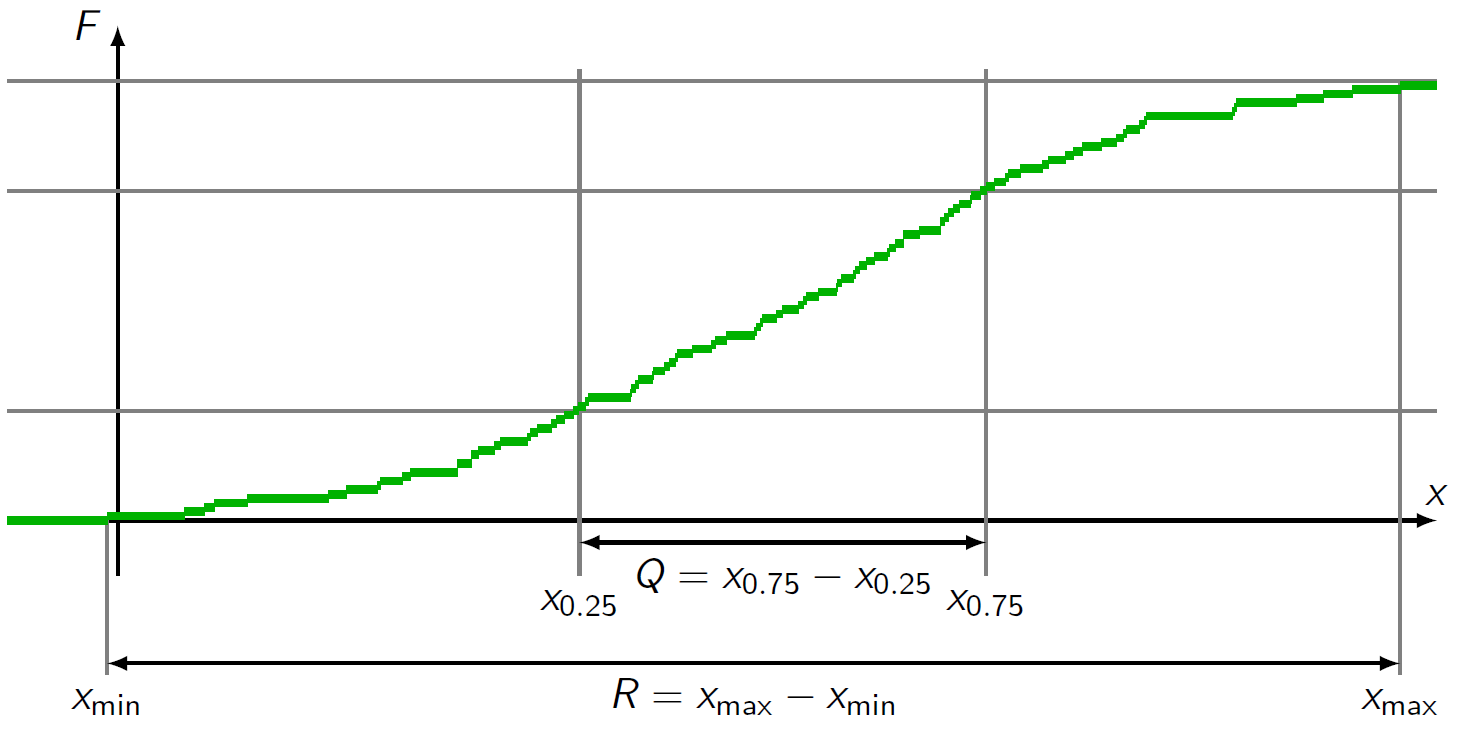
\includegraphics[width=0.65\columnwidth]{images/spannweite_quartilabstand.png}
\end{center}


\subsection[Wahrscheinlichkeitdichte]{Wahrscheinlichkeitdichte $\bm{\varphi(x)}$}

\textbf{Achtung: Nur für stetige Zufallsvariablen}

\vspace{0.2cm}

\begin{minipage}{0.33\columnwidth}
	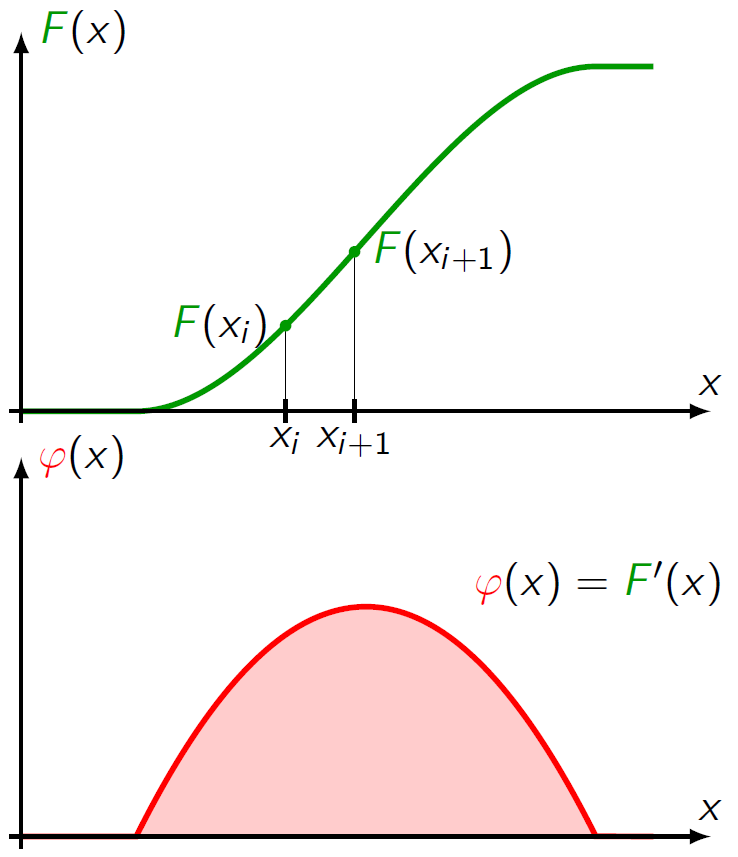
\includegraphics[width=\columnwidth]{images/wahrscheinlichkeitsdichte_1.png}
\end{minipage}
\hfill
\begin{minipage}{0.6\columnwidth}
	\myul{ \textbf{Eigenschaften von $\crd{\varphi}(x)$} }

	\vspace{0.1cm}

	\begin{itemize}
		\item $\crd{\varphi}(x) = \cgn{F}'(x)$
		\item $P(a < X \leq b) = \int\limits_a^b \crd{\varphi}(x) \, \diff x $
		\item $\cgn{F}(x) = \int\limits_{-\infty}^x \varphi(\xi) \, \diff \xi$
		\item $\int\limits_{-\infty}^{\infty} \varphi(x) = 1$ (Normierungsbedingung)
		\item $\varphi(x) \geq 0 \quad \forall \, x \in \mathbb{R}$
	\end{itemize}
\end{minipage}

$$ \varphi_{X+Y}(x) = (\varphi_X * \varphi_Y)(x) = \int\limits_{-\infty}^{\infty} \varphi_X(t) \cdot \varphi_Y(x - t) \, \diff t \quad \text{(Faltung)} $$


\subsection{Erwartungswert mittels Wahrscheinlichkeitsdichte}

\vspace{-0.2cm}
\begin{align*}
	E(\cgn{X})		&= \cbl{\sum} \cgn{\text{Wert}} \times \crd{\text{Wahrscheinlichkeit}} 					\\
					&= \cbl{\int\limits_{-\infty}^{\infty}} \cgn{x} \cdot \crd{\varphi(x) \, \diff x}  		\\
	E(\cgn{X^2}) 	&= \cbl{\int\limits_{-\infty}^{\infty}} \cgn{x^2} \cdot \crd{\varphi(x) \, \diff x} 	\\
	E(\cgn{f(x)}) 	&= \cbl{\int\limits_{-\infty}^{\infty}} \cgn{f(x)} \cdot \crd{\varphi(x) \, \diff x} 
\end{align*} 


\example{Bestimmung $\bm{E(X)}$ im Intervall [a, b]}

\begin{enumerate}
	\setlength\itemsep{1em}

	\item Normierungsbedingung überprüfen \quad $\int\limits_{- \infty}^{\infty} \varphi(x) \, dx \overset{!}{=} 1$
	\item Erwartungswert $E(X)$ bestimmen \quad $E(X) = \int\limits_{-\infty}^{\infty} x \cdot \varphi(x) \, \diff x$
	\item $E(X^2)$ berechnen \quad $E(X^2) = \int\limits_{-\infty}^{\infty} x^2 \cdot \varphi(x) \, \diff x$
	\item Varianz berechnen \quad $\sigma^2 = \var(x) = E(X^2) - E(X)^2$
	\item Wurzel der Varianz berechnen (und ev. einzeichnen)
\end{enumerate}


		\section{Katalog Wahrscheinlichkeitsverteilungen}

\subsection[Übersicht Zufallsprozesse -- Verteilungen]{Übersicht Zufallsprozesse \textrightarrow\ Verteilungen}

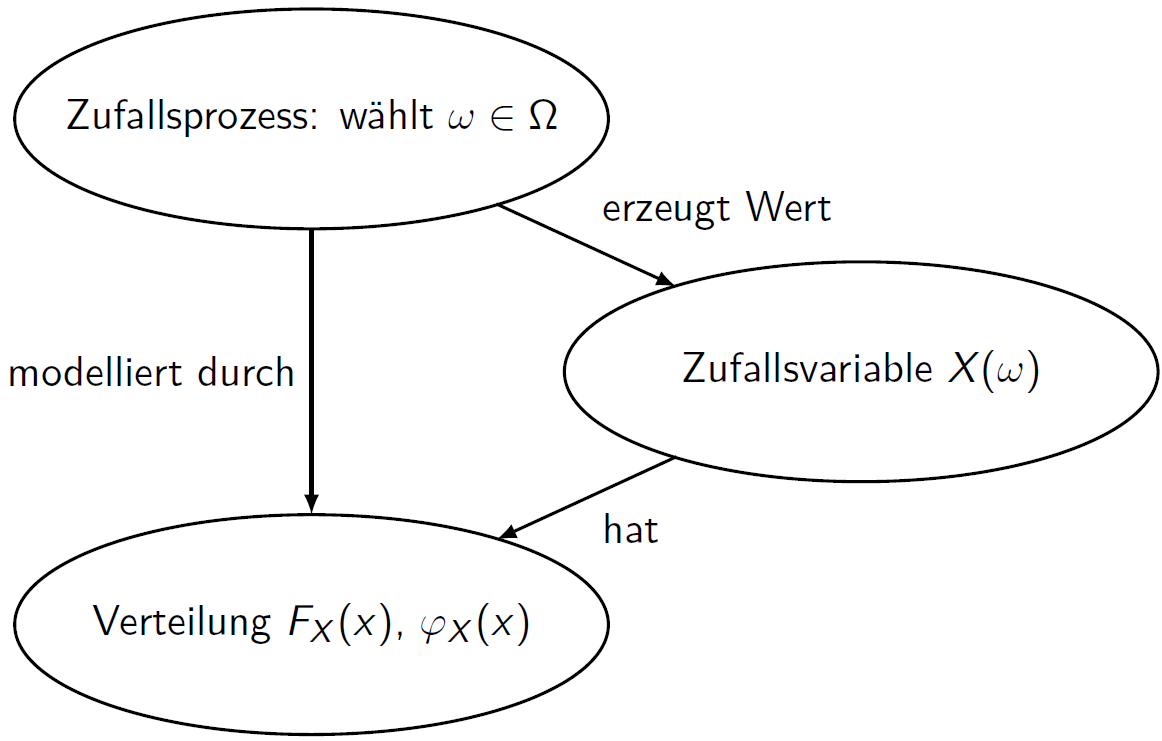
\includegraphics[width=0.5\columnwidth]{images/uebersicht_zufallsprozesse_verteilung}

% Platz für eigene Notizen...


\subsection{Gedächtnislose Prozesse}

\subsubsection{Definition}

Die positive Zufallsvariable $T$ ist der Zeitpukt, zu dem ein Ereignis eintritt

\vspace{0.2cm}

\begin{minipage}{0.38\columnwidth}
	$$ \boxed{ F(x) = P( T \leq x ) } $$
\end{minipage}
\hfill
\begin{minipage}{0.58\columnwidth}
	$$ \boxed{ G(x) = 1 - F(x) = P(T > x) } $$
\end{minipage}


\subsubsection{Gedächtnislos}

$T$ ist gedächtnislos, wenn die Wahrscheinlichkeit, dass das Ereignis in einem Intervall eintritt, immer gleich gross ist, 
wenn es zu Beginn des Intervalls noch nicht eingetreten ist \\
\textbf{Bei gedächtnislosen Prozessen hat die Vergangenheit keinen Einfluss auf den Ausgang eines Experiments / Prozesses }

$$ \cbl{P(T \leq x+y \, | \, T > x)} = \cgn{P(T \leq y)} $$

\cgn{Wahrscheinlichkeit, dass Ereingnis jetzt eintritt} \\
\cbl{Wahrscheinlichkeit, dass Ereingnis später eintritt}

\vspace{0.1cm}

\textrightarrow\ \textbf{Exponentialverteilung} erfüllt diese Bedingung


\subsubsection{Beispiele für Gedächtnislose Prozesse}

\begin{tabular}{lll}
	\tabitem Etwas geht kaputt	& \tabitem Radioaktiver Zerfall	& \tabitem Warteschlangen 
\end{tabular}


\subsection{Exponentialverteilung (gedächtnislos)}

\begin{minipage}[c]{0.46\columnwidth}
	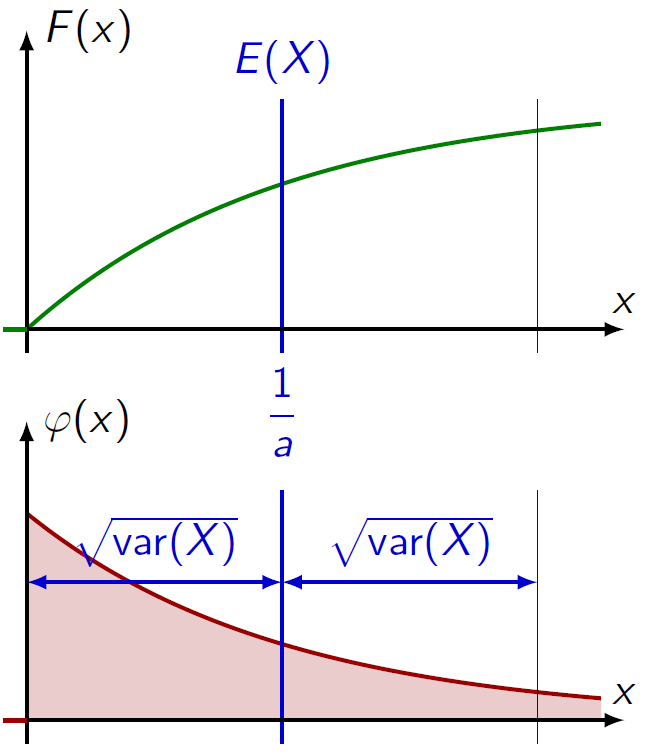
\includegraphics[width=\columnwidth]{images/exponentialverteilung.png}
\end{minipage}
\hfill
	\begin{minipage}[c]{0.52\columnwidth}
	$\cgn{F(x)} = \begin{cases} 
		0 				& x \leq 0 \\
		1 - e^{-a\, x} 	& x > 0 
	\end{cases}$

	\vspace{0.3cm}

	$\crd{\varphi(x)} = \begin{cases} 
		0 					& x \leq 0 \\
		a \, e^{-a \, x} 	& x > 0 
	\end{cases}$ 

	\vspace{0.3cm}

	Parameter: \quad $a$, $\frac{1}{a}$

	\vspace{0.2cm}

	$\frac{1}{a} = $ MTBF (Mean Time Between Failure) \\
	\textbf{( \textrightarrow\ mittlere Lebnsdauer)}
\end{minipage}


\subsubsection{Eigenschaften der Exponentialverteilung}

\myul{\textbf{Erwartungswert $\bm{E(X)}$}}
$$ \boxed{ E(X) = \frac{1}{a} = \text{MTBF (mittlere Lebensdauer)} } $$

\myul{\textbf{Varianz $\bm{\var(x)}$}}

\vspace{0.2cm}

\begin{minipage}[c]{0.6\columnwidth}
	$$ \boxed{ \sigma^2 = \var(x) = E(X^2) - E(X)^2 = \frac{1}{a^2} } $$
\end{minipage}
\hfill
\begin{minipage}[c]{0.36\columnwidth}
	$$ \boxed{E(X^2) = \frac{2}{a^2} } $$
\end{minipage}

\vspace{0.2cm}

\myul{\textbf{Median (Halbwertszeit) }} $\bm{t_{\frac{1}{2}}}$

\begin{minipage}[c]{0.48\columnwidth}
	$$ P(T \leq t_{\frac{1}{2}} ) = \frac{1}{2} $$
\end{minipage}
\hfill
\begin{minipage}[c]{0.48\columnwidth}
	$$ \boxed{ t_{\frac{1}{2}} = \frac{\ln(2)}{a} } $$
\end{minipage}


\subsubsection{Anwendungen}

\begin{tabular}{ll}
	\tabitem Prozess ohne Erinnerungsvermögen	& \tabitem Radioaktivität
\end{tabular}


\subsection{Erlang-Verteilung}

\subsubsection{Voraussetzungen}

$X_i$ ist eine \textbf{unabhängige exponentialverteilte} Zufallsvariable mit Parameter $a$


\subsubsection{Definition der Erlang-Verteilung}

\begin{minipage}[c]{0.48\columnwidth}
	$\crd{\varphi_k(x)} = \begin{cases} 
		0 											& x < 0 \\
		a^k \, \frac{x^{k-1}}{(k-1)!}\, e^{-a \, x} & x \geq 0 
	\end{cases}$ 
\end{minipage}
\hfill
\begin{minipage}[c]{0.48\columnwidth}
	$k = 1$: Exponentialverteilung
\end{minipage}


\subsubsection{Eigenschaften der Erlang-Verteilung}

\myul{\textbf{Verteilungsfunktion $\bm{\varphi_{k+1}(x)}$ von $\bm{T_1 + T_k}$}}
$$ \boxed{ \varphi_{k+1}(x) = \varphi_k * \varphi_1 = a^{k+1} \, \frac{x^k}{k!} \, e^{-a \, x} } $$

\myul{\textbf{Summe von Erwartungswerten $\bm{E(T_1 + T_2)}$}}
$$ \boxed{ E(T_1 + T_2) = E(T_1) + E(T_2) = \frac{1}{a} + \frac{1}{a} = \frac{2}{a} } $$


\subsubsection{Anwendungen}

\begin{tabular}{lll}
	\tabitem Wartezeit in Telefonzentrale / am Postschalter	& \tabitem Warteschlangenprobleme
\end{tabular}


\subsection{Poisson-Verteilung}

\subsubsection{Voraussetzung}

Gedächtnislose Prozesse $T_i$ mit gleichem Parameter $a$


\subsubsection{Aufgabe}

Wie gross ist die Wahrscheinlichkeit, dass in einem Intervall der Länge $x$ genau $k$ Ereignisse / Prozesse stattfinden?
$$ P( S_k \leq x \wedge S_{k+1} > x) = F_k(x) - F_{k+1}(x) \quad \text{mit } S_k = T_1 + ... + T_k $$


\subsubsection{Poisson-Verteilung}

\begin{minipage}{0.36\columnwidth}
	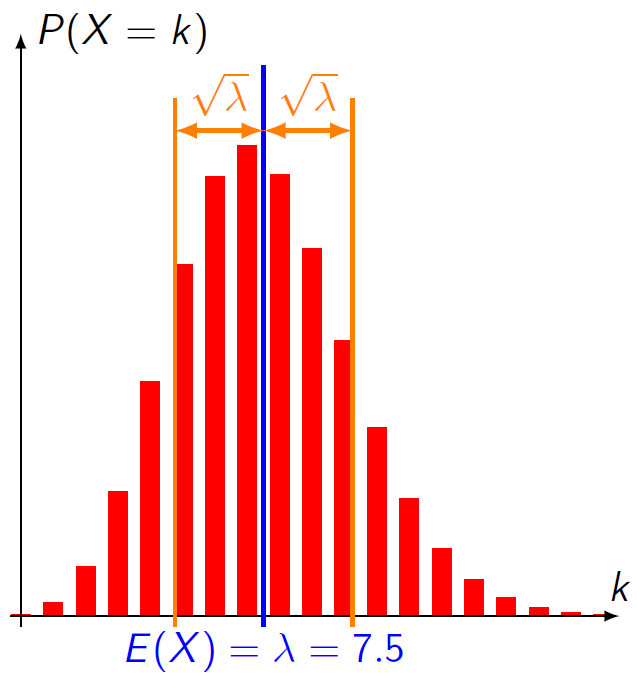
\includegraphics[width=\columnwidth]{images/poissonverteilung.png}
\end{minipage}
\hfill
\begin{minipage}{0.6\columnwidth}
	\begin{align*}
		P_k(\lambda)	&= F_k(x) - F_{k+1}(x)					\\
						&= e^{-a \, x} \frac{(a \, x )^k}{k!} 	\\
		P_k(\lambda) 	&= e^{- \lambda} \frac{\lambda^k}{k!}
	\end{align*}

	Parameter: $\lambda = a \, x$ \\
	(erwartete \# Ereignisse im Intervall $x$)
\end{minipage}


\subsubsection{Eigenschaften der Poisson-Verteilung}

Die Poisson-Verteilung ist eine \textbf{diskrete Verteilung}

\vspace{0.2cm}

\myul{\textbf{Erwartungswert $\bm{E(X)}$}}
\vspace{0.1cm}
$$ \boxed{\lambda = E(X) = a \cdot x } $$

\vspace{0.2cm}

\myul{\textbf{Varianz $\bm{\var(x)}$}}
\vspace{0.1cm}
$$ \boxed{ \sigma^2 = \var(x) = \lambda = a \cdot x } $$

\vspace{0.2cm}

\myul{\textbf{Summe von Wahrscheinlichkeiten (z.B. $\bm{P(k \leq 3)}$) }} 
$$ \boxed{ P(k \leq 3) = e^{-\lambda} \sum\limits_{k=0}^3 \frac{\lambda^k}{k!} } $$


\subsubsection{Anwendungen}

\begin{itemize}
	\item Anzahl Ereignisse mit exponentialverteilten Intervallen
	\item Approximation der Binomialverteilung für seltene Ereignisse, die mit Rate $\lambda$ eintreten
\end{itemize}


\subsection[Zufallszahlen mit Verteilung F(x)]{Zufallszahlen mit Verteilung $F(x)$}

\subsubsection{Voraussetzung}

$F(X)$ ist eine Verteilungsfunktion, $X$ ein im Intervall $[0,1]$ gleichverteilte Zufallsvariable


\subsubsection{Verteilungsfunktion von $Z$}

\begin{minipage}{0.25\columnwidth}
	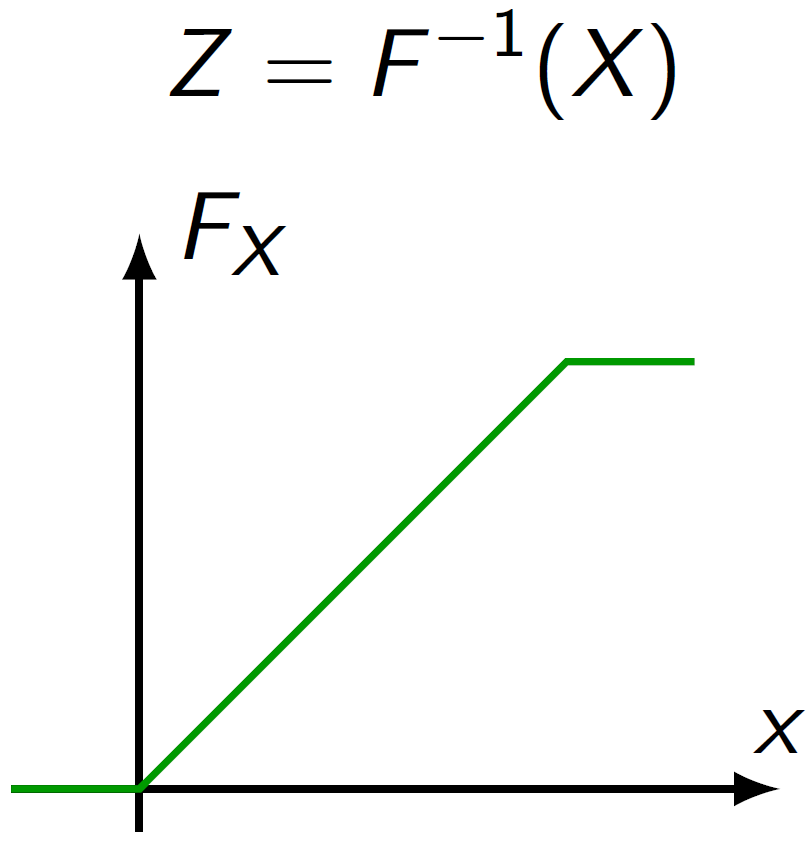
\includegraphics[width=\columnwidth]{images/verteilung_F(x).png}
\end{minipage}
\hfill
\begin{minipage}{0.7\columnwidth}
	\renewcommand{\arraystretch}{1.3}
	\begin{tabular}{r l l}
		$F_Z(z)$ 	& $= P( Z \leq z)$ 			& Definition $F_z$	\\
					& $= P(F^{-1}(X) \leq z)$ 	& Definition $Z$ 	\\
					& $= P(X \leq F(z))$ 		& Umformung 		\\
					& $= F_X(F(z))$ 			& Definition $F_X$ 	\\
					& $= F(z)$   
	\end{tabular}
	\renewcommand{\arraystretch}{1}
\end{minipage}


\subsection{Normalverteilung}

Es geht um eine \textbf{Summe vieler kleiner Einflüsse}

\vspace{0.2cm}

\begin{minipage}{0.4\columnwidth}
	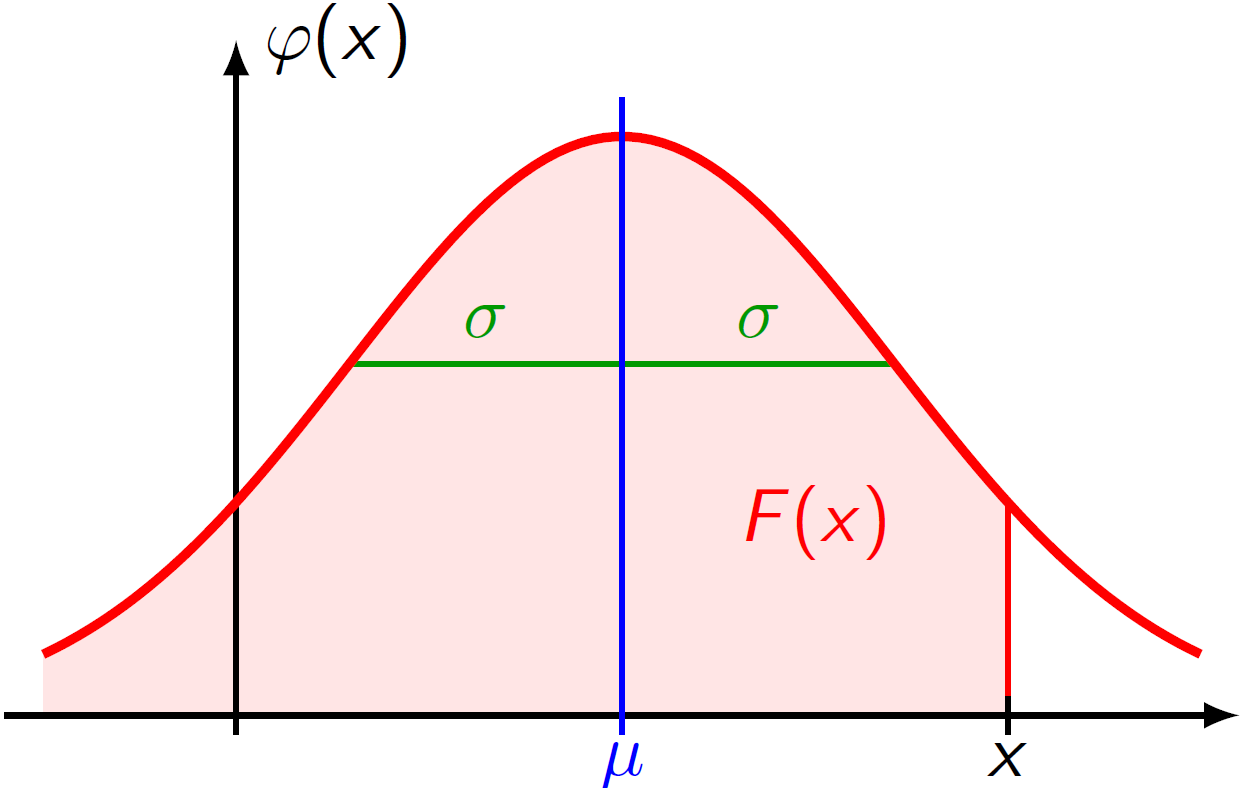
\includegraphics[width=\columnwidth]{images/normalverteilung.png}
	Maximum bei $x = \mu$ \\
	Wendepunkte bei $x = \mu \pm \sigma$ 
\end{minipage}
\hfill
\begin{minipage}{0.48\columnwidth}
	$X$ heisst \textbf{normalverteilt}, mit $E(X) = \mu$ und $\var(X) = \sigma^2$, $N(\mu, \sigma^2)$, wenn sie folgende 
	Wahrscheinlichkeitsdichte $\varphi(x)$ hat:
	$$ \boxed{ \varphi(x) = \frac{1}{\sigma \sqrt{2 \pi}} e^{- \frac{(x - \mu)^2}{2 \sigma^2}} } $$

	$\mu$ \quad Erwartungswert \\
	$\sigma$ \quad Standardabweichung 
\end{minipage}


\subsubsection{Typische Werte der Normalverteilung}

\begin{minipage}{0.45\columnwidth}
	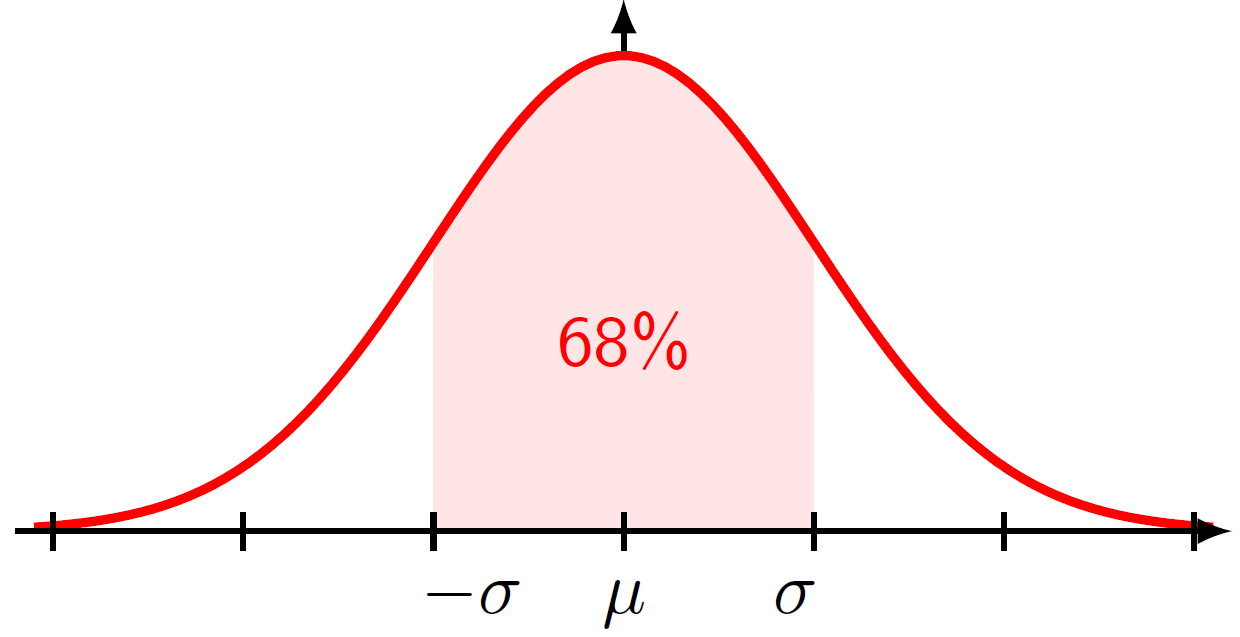
\includegraphics[width=\columnwidth]{images/normalverteilung_typische_werte.png}
\end{minipage}
\hfill
\begin{minipage}{0.45\columnwidth}
	\begin{tabular}{l c l}
		$\pm \, 1 \, \sigma$ & \textrightarrow\ & $68 \, \%$ 	\\
		$\pm \, 2 \, \sigma$ & \textrightarrow\ & $95 \, \%$ 	\\
		$\pm \, 3 \, \sigma$ & \textrightarrow\ & $99.7 \, \%$
	\end{tabular}
\end{minipage}


\subsubsection{Eigenschaften der Normalverteilung}

\myul{\textbf{Wahrscheinlichkeit}}

\vspace{0.1cm}

Wahrscheinlichkeit dafür, dass $X$ zwischen $a$ und $b$ liegt:
$$ P(a < X \leq b) = \frac{1}{\sigma \sqrt{2 \pi}} \int\limits_a^b e^{- \frac{(x - \mu)^2}{2 \sigma^2}}  \, \diff x $$


\myul{\textbf{Keine Stammfunktion}}

\vspace{0.1cm}

Die Wahscheinlichkeitsdichte $\varphi(x)$ der Normalverteilung hat keine Stammfunktion in geschlossener Form\\ 
\textrightarrow\ Nur numerische Berechnungen möglich oder \textbf{Tabellen} verwenden

\vspace{0.2cm}

\myul{\textbf{Symmetrie}}

\vspace{0.1cm}

Die Wahscheinlichkeitsdichte $\varphi(x)$ ist \textbf{symmetrisch} bezüglich $x = \mu$ \\
\textrightarrow\ Erwartungswert $E(X) = \mu$


\subsubsection{Anwendungen}

\begin{itemize}
	\item \textbf{Summe vieler kleiner Einflüsse} vergl. grosse Varianz
	\item Messwerte
	\item Approximation der Binomialverteilung
\end{itemize}


\subsection{Standardnormalverteilung}

\subsubsection{Standardisierung}

$X$ normalverteilt, mit $E(X) = \mu$, $\var(X) = \sigma^2$, dann ist $Z$ normalverteilt:

\vspace{0.2cm}

\begin{minipage}[t]{0.48\columnwidth}
	$$ \boxed{ Z = \frac{X - \mu}{\sigma} } $$
\end{minipage}
\hfill
\begin{minipage}[t]{0.48\columnwidth}
	\myul{\textbf{Eigenschaften}}

	\vspace{0.1cm}

	\begin{itemize}
		\item $E(Z) = 0$
		\item $\var(Z) = 1$
	\end{itemize}
\end{minipage}


\subsubsection{Verteilungsfunktion $\Phi$  der Standardnormalverteilung}

\begin{minipage}{0.48\columnwidth}	
	$$ \boxed{ \Phi(z) = P(Z \leq z) } $$
\end{minipage}
\hfill
\begin{minipage}{0.48\columnwidth}
	$$ \boxed{ \Phi(-z) = 1 -  \Phi(z) } $$
\end{minipage}


\example{Standardnormalverteilung}

\vspace{-0.4cm}

\begin{align*}
	P(\cbl{a} < X \leq \cor{b})	&= P \left( \frac{\cbl{a} - \mu}{\sigma} < \frac{X - \mu}{\sigma} \leq \frac{\cor{b} - \mu}{\sigma}  \right) 	\\
								&= P \left( \frac{\cbl{a} - \mu}{\sigma}  < Z \leq \frac{\cor{b} - \mu}{\sigma} \right) 						\\
								&= \Phi \Bigg( \frac{\cor{b} - \mu}{\sigma} \Bigg) -  \Phi \Bigg( \frac{\cbl{a} - \mu}{\sigma} \Bigg)
\end{align*}

\textrightarrow\ \textbf{Auswertung von $\bm{\Phi()}$ mittels Tabelle in Abschnitt \ref{Verteilungsfunktion der Normalverteilung} } \\
\textrightarrow\ \textbf{Kompakte $\bm{\Phi()}$-Tabelle in Abschnitt \ref{Quantilentabelle der Standardnormalverteilung} } 


\subsubsection{Quantilentabelle der Standardnormalverteilung / TR-Befehle}
\label{Quantilentabelle der Standardnormalverteilung}

\begin{minipage}[c]{0.4\columnwidth}

	\begin{tabular}{|l|r|}
		\hline
		$p$		&	$x$		\\
		\hline
		0.75	&	0.6745	\\
		0.8		&	0.8416	\\
		0.9		&	1.2816	\\
		0.95	&	1.6449	\\
		0.975	&	1.9600	\\
		0.99	&	2.3263	\\
		0.995	&	2.5758	\\
		0.999	&	3.0902	\\
		0.9995	&	3.2905	\\
		\hline
	\end{tabular}
\end{minipage}
\hfill
\begin{minipage}[c]{0.57\columnwidth}
	\myul{\textbf{TI-nspire Befehle (Scratchpad)}}

	\vspace{0.2cm}

	\begin{tabular}{ll}
		$\Phi(x)$ 		& normCdf($\cbl{a}$, $\cor{b}$, $\mu$, $\sigma$)	\\
						& menu-6-5-2										\\
		\\
		$\Phi^{-1}(p)$ 	& invNorm($p$)										\\
						& menu-6-5-3
	\end{tabular}
\end{minipage}


\subsubsection{Rechenregeln Standardnormalverteilung}

\myul{\textbf{Varianz $\bm{\var(X)}$}}
$$ \boxed{ \sigma^2 = \var(X) = E(X^2) - E(X)^2 } $$ 


\myul{\textbf{Summensatz $ \bm{X = X_1 + X_2}$}}

\vspace{0.1cm}
$X_1$ normalverteilt mit $E(X_1) = \mu_1$ und $\var(X_1) = \sigma_1^2$, \\
$X_2$ normalverteilt mit $E(X_2) = \mu_2$ und $\var(X_2) = \sigma_2^2$, \\
dann ist $X = X_1 + X_2$ normalverteilt mit:

\vspace{0.2cm}

\begin{minipage}[c]{0.48\columnwidth}
	$$ \boxed{ E(X) = \mu_1 + \mu_2 } $$
\end{minipage}
\hfill
\begin{minipage}[c]{0.48\columnwidth}
	$$ \boxed{ \sigma^2 = \var(X)  = \sigma_1^2 + \sigma_2^2 } $$
\end{minipage}

\vspace{0.2cm}

\myul{\textbf{Linearität}}

\vspace{0.1cm}

$X$ normalverteilt mit $E(X) = \mu$ und $\var(X) = \sigma^2$, dann ist $a \, X + b$ normalverteilt mit:

\vspace{0.2cm}

\begin{minipage}[c]{0.48\columnwidth}
	$$ \boxed{ E(a \, X + b) = a \, \mu +  b } $$
\end{minipage}
\hfill
\begin{minipage}[c]{0.48\columnwidth}
	$$ \boxed{ \var(a \, X + b)  = a^2 \, \sigma^2 }  $$
\end{minipage}



\subsection[Bestimmung der Parameter]{Bestimmung der Parameter $\bm{\mu}$, $\bm{\sigma^2}$}

\subsubsection{Schätzen}

\vspace{-0.2cm}

$$\hat{\mu} = E(X) = \frac{1}{n} \sum\limits_{i=1}^n x_i \text{  (Mittelwert)}$$
$$\hat{\sigma}^2 = \cor{\frac{n}{n-1}} \, (  E(X^2) - E(X)^2 ) = \cor{\frac{n}{n-1}} \, \left( \frac{1}{n} \sum\limits_{i=1}^n x_i^2 - \Big( \frac{1}{n} \sum\limits_{i=1}^n x_i  \Big)^2  \right) $$

\cor{Korrektur, damit erwartungstreu}


\subsubsection{Wahrscheinlichkeit (Standardnormalverteilung)}

$X \leq x$ mit Wahrscheinlichkeit $p$

\begin{align*}
	P(X \leq x) 														&= p 						\\
	P \Big( \frac{X - \mu}{\sigma} \leq \frac{x - \mu}{\sigma} \Big) 	&= p 						\\
	P \Big( Z \leq \frac{x - \mu}{\sigma} \Big) 						&= p 						\\
	\Phi \Big( \frac{x - \mu}{\sigma} \Big) 							&= p 						\\
	x - \mu 															&= \sigma \, \Phi^{-1}(p) 	\\
	\mu + \Phi^{-1}(p) \, \sigma 										&= x 
\end{align*}

Spezialfall Median: $p = 0.5$ \qquad  $\Phi^{-1}(0.5) = 0$ \qquad \textrightarrow\ $\mu = x$


\subsection{Zentraler Grenzwertsatz (Normalverteilung)}

Sind $X_1$, $X_2, \, \ldots$ identisch verteilte und unabhängige Zufallsvariablen mit $E(X_i) = \mu$ und \\
$\var(X_i) = \sigma^2$, dann gilt:

\renewcommand{\arraystretch}{2}
\begin{tabular}{l c l l}
	$S_n = \sum\limits_{i=1}^n X_i$ 				& \textrightarrow\	& $E(S_n) = n \, \mu$ 	& $\var(S_n) = n \, \sigma^2$	\\
	$Z_n = \frac{S_n - n \, \mu}{\sqrt{n} \sigma}$ 	& \textrightarrow\ 	& $E(Z_n) = 0$ 			& $\var(Z_n) = 1$
\end{tabular}
\renewcommand{\arraystretch}{1}

\vspace{0.2cm}
Für $n \to \infty$ strebt die Verteilung von $Z_n$ gegen die Standardnormalverteilung, d.h. 
$$ \lim\limits_{n \to \infty} P(Z_N \leq z) = \Phi(z) $$
\textbf{\textrightarrow\ Die Summe vieler vergleichbarer kleiner Einflüsse ist annähern normalverteilt}


\subsubsection{Spezielfall Standardnormalverteilung}

$X_i$ Zufallsvariablen mit $E(X_i) = 0$ und $\var(X_i) = 1$, dann konvergiert die Verteilungsfunktion $S_n$
gegen eine Normalverteilung mit $\mu = 0$ und $\sigma = 1$
$$ S_n = \frac{X_1 + \ldots + X_n}{\sqrt{n}} $$
\textbf{\textrightarrow\ Viele kleine Einflüsse ergeben zusammen immer eine Normalverteilung!}

\columnbreak


\subsection{Binomialverteilung}

\subsubsection{Voraussetzungen}

Zufallsexperiment mit \textbf{zwei} möglichen Ausgängen $A$ oder $\overline{A}$ mit \\
Wahrscheinlichkeit $p = P(A)$


\subsubsection{Binomialverteilung}

$X =$ Anzahl Eintreten von $A$ in $n$ \textbf{unabhängigen} Durchführungen

$$ \boxed{ P( X = k ) = \begin{pmatrix} n \\ k \end{pmatrix} p^k (1-p)^{n-k} } $$

\textbf{Notation: } $X \sim \Bi(n, p)$ \\
Taschenrechner Binomialkoeffizient: nCr($n, \, k$) \\
Taschenrechner Binomialverteilung: binomPdf($n, \, p, \,k$)


\subsubsection{Eigenschaften der Binomialverteilung}

\myul{\textbf{Erwartungswert $E(X)$}}

\vspace{0.1cm}

$$ \boxed{ \mu =  E(X) = n \, p } $$

\vspace{0.2cm}

\myul{\textbf{Varianz $\bm{\var(x)}$}}

\vspace{0.1cm}

$$ \boxed{ \sigma^2 = \var(x) = n \, p \, (1 - p) } $$


\subsubsection{Anwendungen}

\begin{itemize}
	\item Anzahl Eintreten eines Bernoulliexperimentes 
\end{itemize}


\subsection{Normalapproximation der Binomialverteilung}

$X$ ist Summe von $n$ kleinen Einflüssen auf das Gesamte \\
\textrightarrow\ $P(X \leq k)$ kann mit der \textbf{Normalverteilung} approximiert werden, sofern die 
\textbf{Anzahl Wiederholungen $\bm{n}$ gross genug} ist und man sich nahe beim 'Buckel' der Normalverteilung befindet

\vspace{0.2cm}

\begin{minipage}[c]{0.48\columnwidth}
	$$ \boxed{ \mu = E(X) = n \, p } $$
\end{minipage}
\hfill
\begin{minipage}[c]{0.48\columnwidth}
	$$ \boxed{ \sigma^2 = \var(X) = n \, p \, (1 - p) } $$
\end{minipage}

\vspace{0.2cm}

$$ \text{ \textrightarrow\ } \frac{X - \mu}{\sigma} = \frac{X - n \, p}{\sqrt{n \, p \, (1 - p)}} \quad \text{ angenähert standardnormalverteilt} $$


\subsubsection{Standardisierung (ohne Korrektur)}

\vspace{-0.4cm}

\begin{align*}
	P(\cbl{a} < X \leq \cor{b}) &= P \left( \frac{\cbl{a} - n \, p}{\sqrt{n p \, (1 - p)}} < \frac{X - n p}{\sqrt{n p (1 - p)}} \leq \frac{\cor{b} - n p}{\sqrt{n p (1 - p)}}  \right) 	\\
								&= P \left( \frac{\cbl{a} - n  p}{\sqrt{n p (1 - p)}}  < Z \leq \frac{\cor{b} - n p}{\sqrt{n p (1 - p)}} \right) 											\\
								&= \Phi \left(  \frac{\cor{b} - n p}{\sqrt{n p (1 - p)}} \right) -  \Phi \left( \frac{\cbl{a} - n p}{\sqrt{n p (1 - p)}} \right)
\end{align*}

\textrightarrow\ \textbf{Auswertung von $\bm{\Phi()}$ mittels Tabelle Abschnitt \ref{Verteilungsfunktion der Normalverteilung}}


\subsubsection{Standardisierung mit Korrektur (Prüfung!)} 

Für eine noch genauerere Approximation kann folgende Korrektur eingefügt werden:

\vspace{-0.2cm}

\begin{align*}
	P(a \, \crd{<} \,  X \,  \cor{\leq} \, b) 	&= \Phi \left( \frac{b \cor{+ \frac{1}{2}} - n \, p}{\sqrt{n p \, (1 - p)}} \right) - \Phi \left( \frac{a \crd{+ \frac{1}{2}} - n p}{\sqrt{n p (1 - p)}} \right) \\
	P(a \, \cgn{\leq} \, X \, \cbl{\leq} \, b) 	&= \Phi \left( \frac{b \cbl{+ \frac{1}{2}} - n \, p}{\sqrt{n p \, (1 - p)}} \right) - \Phi \left( \frac{a \cgn{- \frac{1}{2}} - n p}{\sqrt{n p (1 - p)}} \right)
\end{align*}


\subsubsection{Vergleich \crd{Binomialverteilung} -- \cbl{Normalverteilung}}

\begin{center}
	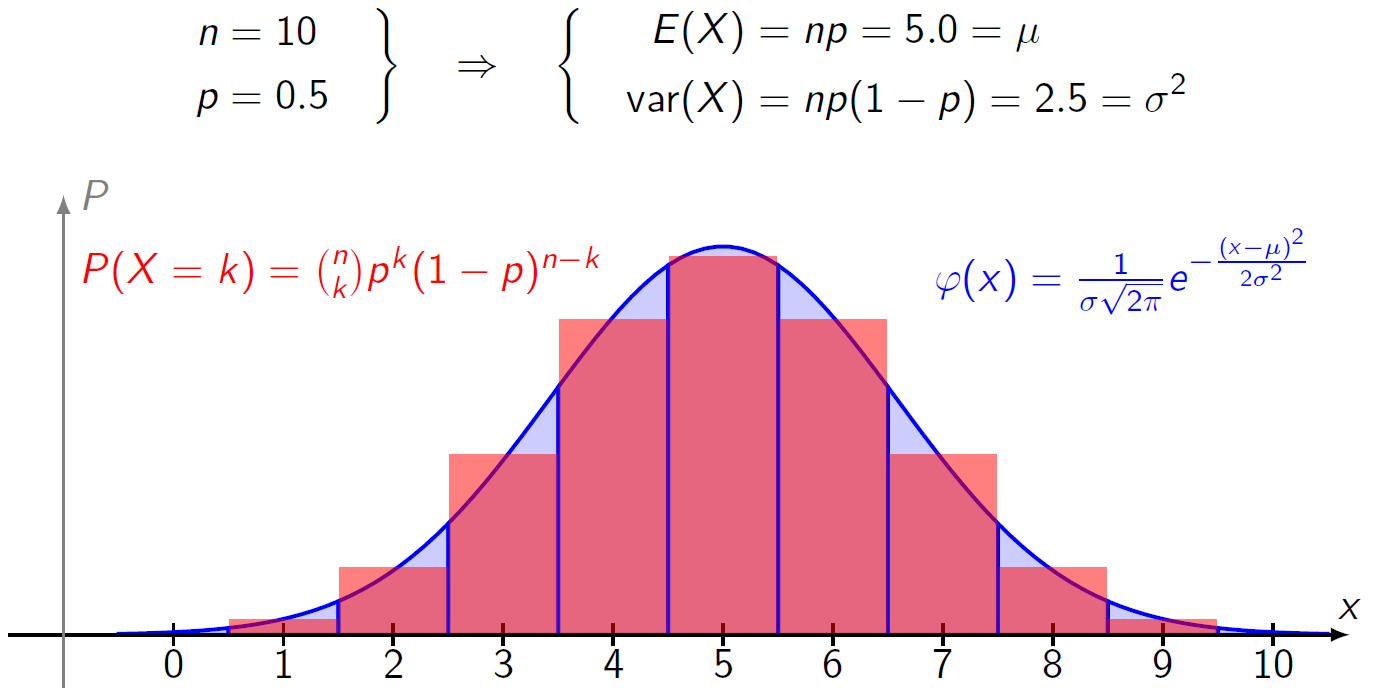
\includegraphics[width=0.75\columnwidth]{images/binomialverteilung_normalverteilung.png}
\end{center}


\columnbreak


\subsection{Approximation für \textbf{seltene} Ereignisse (Poisson)}

\subsubsection{Voraussetzungen}

Grenzwert $n \to \infty$ mit $n \cdot p = \lambda = $ erwartete Anzahl Ereignisse konstant (d.h. $p \to 0$) \\
\textbf{Wenn an der Prüfung \crd{SELTEN} in der Aufgabenstellung steht!!}

$$ \boxed{ P(X = k) = \begin{pmatrix} n \\ k \end{pmatrix} p^k (1-p)^{n-k} = e^{- \lambda} \frac{\lambda^k}{k!} = P_{\lambda}(k) } $$

Parameter: $\lambda = n \cdot p$ \quad (erwartete \# Ereignisse im Intervall $x$)

\vspace{0.2cm}

\myul{\textbf{Poissson - Summe von Wahrscheinlichkeiten (z.B. $\bm{P(k \leq 3)}$) }}
$$ \boxed{ P(k \leq 3) = e^{-\lambda} \sum\limits_{k=0}^3 \frac{\lambda^k}{k!} } $$


\subsection{Hypergeometrische Verteilung}

\subsubsection{Voraussetung}

Von $N$ Objekten sind $M$ markiert. Daraus werden $n$ Objekte zufällig ausgewählt.


\subsubsection{Hypergeometrische Verteilung}

$X = $ Anzahl markierte Objekte unter den zufällig ausgewählten $n$ Objekten \\
Die Wahrscheinlichkeit, dass \textbf{genau $\boldsymbol{m}$ markierte Objekte gezogen} werden lautet:
$$ \boxed{ P(X = m) = \frac{ \begin{pmatrix} M \\ m \end{pmatrix} \begin{pmatrix} N-M \\ n-m \end{pmatrix} }{\begin{pmatrix} N \\ n \end{pmatrix}} } $$
\textbf{Notation: } $X \sim \mathrm{H}(N, M, n) $


\subsubsection{Eigenschaften der Hypergeometrischen Verteilung}

\myul{\textbf{Erwartungswert $\bm{E(X)}$}}

\vspace{0.1cm}

$$ \boxed{ \mu =  E(X) = n \, \frac{M}{N} } $$ 

\vspace{0.2cm}

\myul{\textbf{Varianz $\bm{\var(x)}$}}

\vspace{0.1cm}

$$ \boxed{\sigma^2 =  \var(X) = n \, \frac{M}{N} \Big( 1 - \frac{M}{N} \Big) \frac{N-n}{N-1} } $$


\example{Hypergeometrische Verteilung}

In einer Kiste mit 20 Äpfeln sind 5 wurmstichig. \\
Wie gross ist die Wahrscheinlichkeit, in einer Stichprobe von 8 Äpfel 2 wurmstichtige zu finden? \\
$N = 20$, $M = 5$, $n = 8$, $m = 2$

$$ P(X = 2) = \frac{ \begin{pmatrix} 5 \\ 2 \end{pmatrix} \begin{pmatrix} 15 \\ 6 \end{pmatrix} }{\begin{pmatrix} 20 \\ 8 \end{pmatrix}} = 0.3973 $$


\subsubsection{Begründung Hypergeometrische Verteilung}

\begin{minipage}{0.4\columnwidth}
	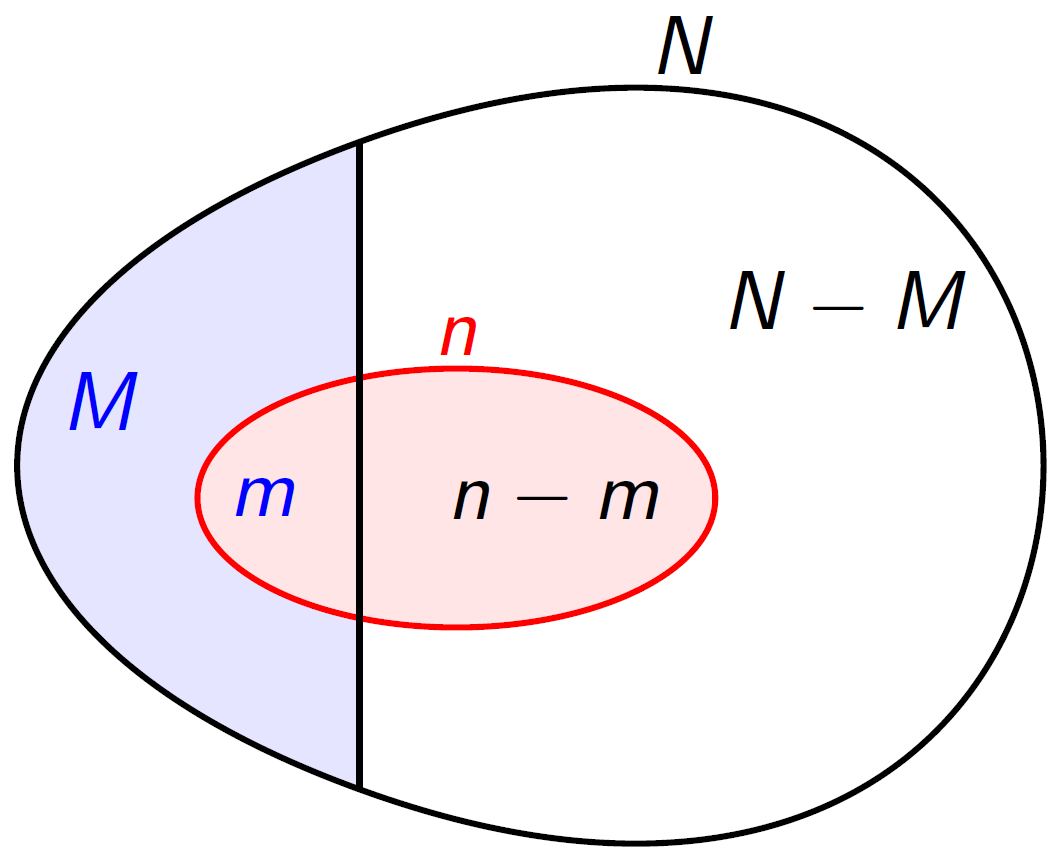
\includegraphics[width=\columnwidth]{images/begruendung_hypergeometrische_verteilung_1.png}
\end{minipage}
\hfill
\begin{minipage}{0.4\columnwidth}
	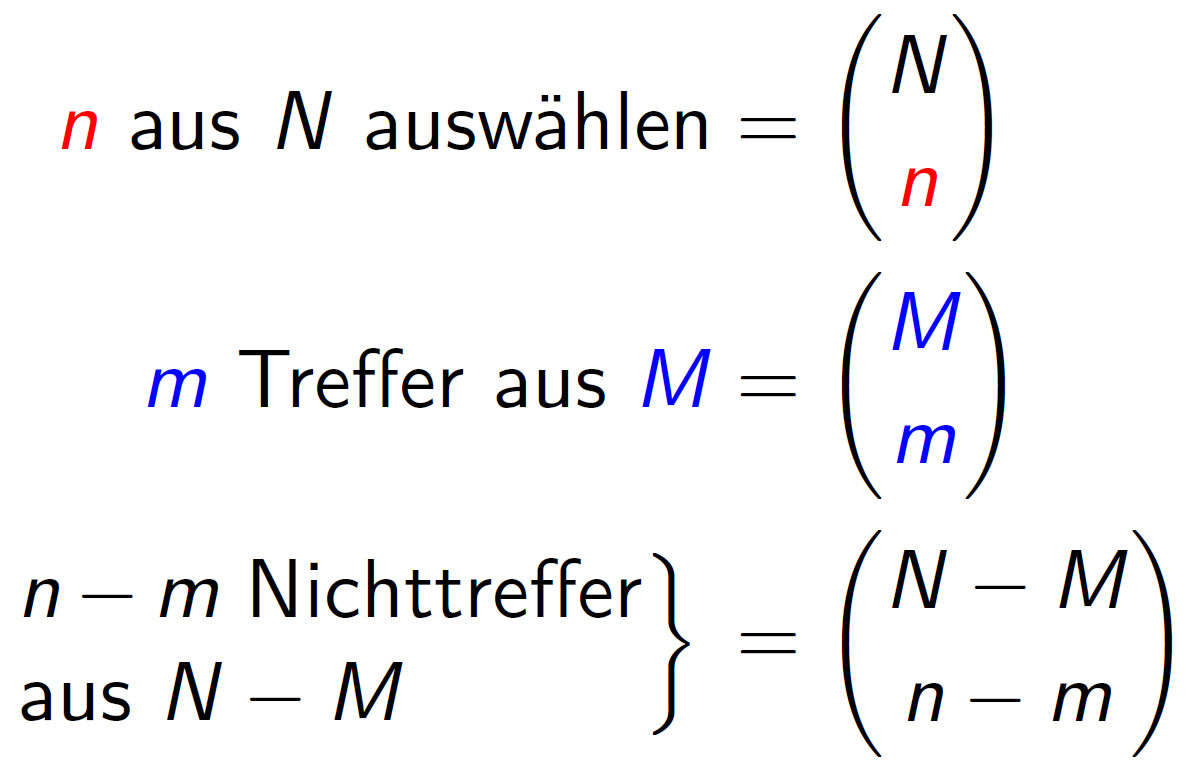
\includegraphics[width=\columnwidth]{images/begruendung_hypergeometrische_verteilung_2.png}
\end{minipage}


\subsection{Potenzverteilung (Skaleninvarianze Prozesse)}

\subsubsection{Skaleninvarianz}

Ein Prozess ist \textbf{skaleninvariant}, wenn er auf jeder Skala \textbf{gleich} abläuft.

\vspace{0.2cm}

Skaliere $x$ mit $b$ \textrightarrow\ Form von $\varphi(x)$ ändert sich nicht

$$ \varphi(bx) = g(b) \, \varphi(x) \quad \text{für } x > x_{\rm min} $$
Faktor $g(b):$ Renormierung


\subsubsection{Potenzverteilung}

\vspace{-0.2cm}

$$ \boxed{ \varphi(x) = C \, e^{- \alpha} \quad \text{mit } \alpha = -g'(1) }$$
Beschränke auf $x > x_{\rm min}$ und wähle $C$ für korrekte Normierung

\vspace{0.2cm}

\begin{minipage}{0.55\columnwidth}
	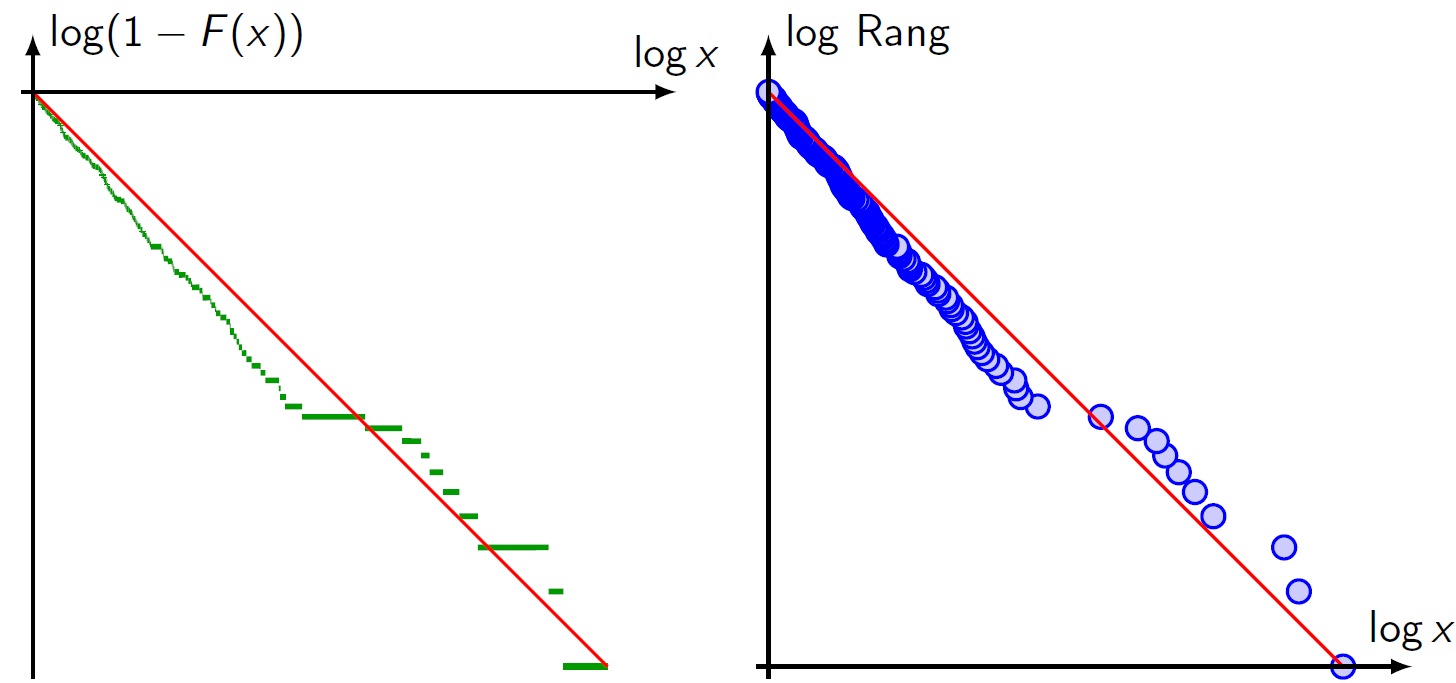
\includegraphics[width=\columnwidth]{images/potenzverteilung.png}
\end{minipage}
\hfill
\begin{minipage}{0.38\columnwidth}
	Geradengleichung in \\
	log-log-Skala
	$$ \log(\varphi(x)) = g'(1) \cdot \log(x) + c $$
\end{minipage}


\subsubsection{Anwendungen}

\begin{minipage}[t]{0.48\columnwidth}
	\begin{itemize}
		\item Städte und Bewohner
		\item Tierarten und ihre Häufigkeit
		\item Mondkrater und Durchmesser
		\item Bücher und Bestseller
	\end{itemize}
\end{minipage}
\hfill
\begin{minipage}[t]{0.48\columnwidth}
	\begin{itemize}
		\item Namen und Häufigkeit
		\item Einkommensverteilung
		\item Skaleninvariante Prozesse
	\end{itemize}
\end{minipage}


\subsubsection{Potenzgesetze für skaleninvariante Prozesse}

\myul{\textbf{Wahrscheinlichkeitsdichte $\bm{\varphi(x)}$}}
$$ \varphi(x) = \begin{cases}
0 																			& x < x_{\rm min} 	\\
\frac{\alpha - 1}{x_{\rm min}} \Big( \frac{x}{x_{\rm min}} \Big)^{-\alpha} 	& x \geq x_{\rm min} 
\end{cases}$$ 


\myul{\textbf{Verteilungsfunktion $\bm{F(x)}$}}

$$ F(x) =  \begin{cases}
0 													& x < x_{\rm min} 		\\
1 - \Big( \frac{x}{x_{\rm min}} \Big)^{1 - \alpha} 	& x \geq x_{\rm min} 
\end{cases}$$ 

\vspace{0.2cm}

\renewcommand{\arraystretch}{1.4}
\begin{tabular}{lll}
	Median 			& $ \mathrm{med}(x) = 2^{\frac{1}{\alpha-1}} \, x_{\rm min} $ 	& für $\alpha > 1$ \\
	Erwartungswert 	& $E(X) = \frac{\alpha - 1}{\alpha - 2} \, x_{\rm min}$ 		& für $\alpha > 2$ \\
	Varianz 		& $ \var(X) = \Big( \frac{\alpha - 1}{\alpha - 3} - \Big( \frac{\alpha - 1}{\alpha - 2} \Big)^2 \Big) \, x_{\rm min}^2 $ & für $\alpha > 3$
\end{tabular}
\renewcommand{\arraystretch}{1}


\subsubsection{'80 / 20 Regel'}

\vspace{-0.4cm}

\begin{minipage}[t]{0.48\columnwidth}
	\begin{align*}
		P(x) 	&= \text{Anteil der Werte } \crd{>} \, x 			\\
				&= 1 - P(X \leq x) = 1 - F(x) 						\\
				&= \int\limits_x^{\infty} \varphi(\xi) \, \diff \xi 
	\end{align*}
\end{minipage}
\hfill
\begin{minipage}[t]{0.48\columnwidth}
	\begin{align*}
		W(x) 	&= \text{Anteil am kumulierten Wert} 									\\
				&= \frac{\int\limits_x^{\infty} \xi \, \varphi(\xi) \, \diff \xi}{E(X)} 
	\end{align*}
	$$ W(x)= P(x)^{\frac{\alpha-2}{\alpha-1}} = P(x)^{\lambda} $$ 
\end{minipage}

\vspace{0.2cm}

\begin{minipage}{0.48\columnwidth}
	$$ \boxed{ \alpha = \frac{\lambda - 2}{\lambda - 1} } $$
\end{minipage}
\hfill
\begin{minipage}{0.48\columnwidth}
	$$ \boxed{ \lambda = \frac{\log(W)}{\log(P)} } $$
\end{minipage}


\subsection{Gleichverteiung}

\begin{minipage}{0.48\columnwidth}
	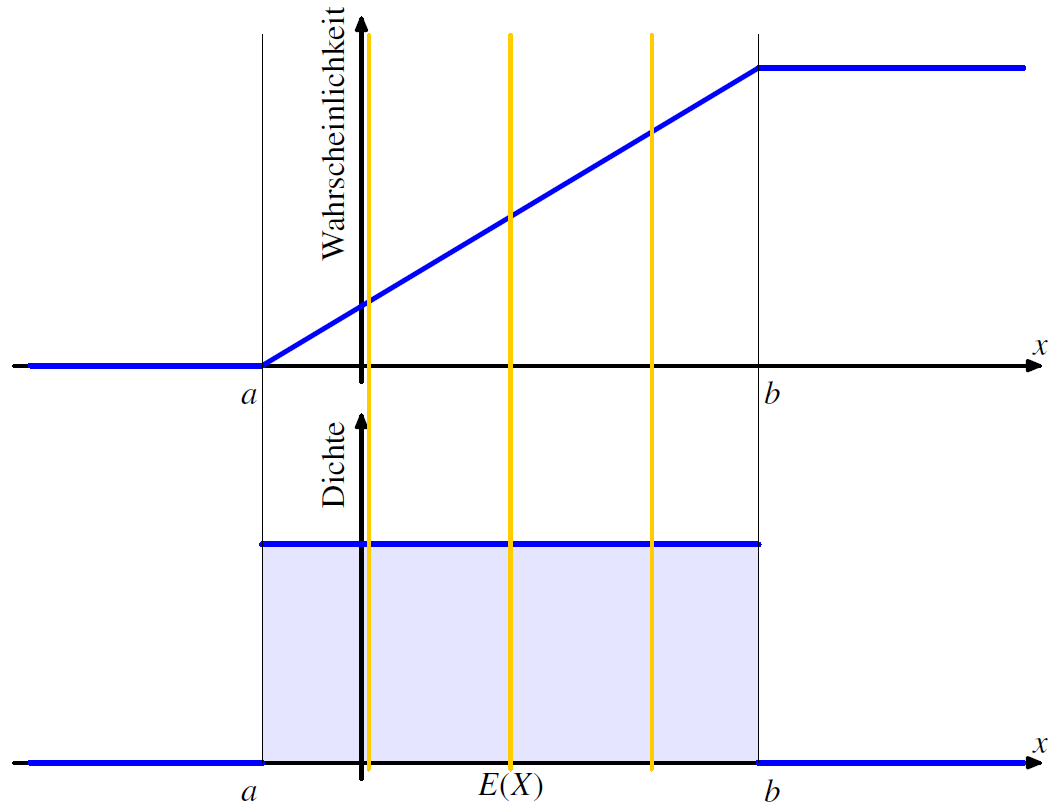
\includegraphics[width=\columnwidth]{images/gleichverteilung.png}
\end{minipage}
\hfill
\begin{minipage}{0.48\columnwidth}
	$\cgn{F(x)} =
	\begin{cases} 
	0 				& x \leq a 			\\
	\frac{x-a}{b-a} & a \leq x \leq b 	\\
	1 				& x > b 
	\end{cases}$ 
	
	\vspace{0.3cm}
	
	$\crd{\varphi(x)} = 
	\begin{cases} 
	\frac{1}{b-a} 	& a \leq x \leq b \\
	0 				& \text{sonst}
	\end{cases}$
\end{minipage}


\subsubsection{Eigenschaften der Gleichverteiung}

\myul{\textbf{Erwartungswert $\bm{E(X)}$}}

$$ \boxed{ E(X) = \frac{a + b}{2}} $$

\vspace{0.2cm}

\textbf{Varianz $\bm{\var(X)}$}

$$ \boxed{\var(X) = \frac{(b - a)^2}{12}} $$


\subsubsection{Anwendungen}

\begin{tabular}{ll}
	\tabitem Verteiung von Zufallszahlen	& \tabitem Keine bevorzugten Werte
\end{tabular}

\columnbreak


		\section{Schätzen}

\subsection{Eigenschaften von Schätzern}

\subsubsection{Konsistenz}

Korrektur für genügend grosse Stichproben
$$ \lim\limits_{n \to \infty} \hat{\vartheta}(x_1, \, \ldots \, , \, x_n) = \vartheta $$


\subsubsection{Erwartungstreu}

Im Mittel korrekt selbst für kleine Stichproben
$$ E (\hat{\vartheta}(X_1, \, ... \, , \, X_n) ) = \vartheta $$


\subsection{Maximum Likelihood Prinzip}

\subsubsection{Aufgabe}

Stichprobe $x1, \, \ldots \, , x_n$ einer normalverteilten Zufallsvariable mit $\sigma = 1$. \\
Schätze den Parameter $\mu$ der Standardnormalverteilung
$$ \cbl{\varphi}(x, \crd{\mu}) = \frac{1}{ \sqrt{2 \pi}} e^{- \frac{(x - \crd{\mu})^2}{2}}  \, \diff x $$


\subsubsection{Likelihood-Funktion}

\begin{minipage}{0.4\columnwidth}
    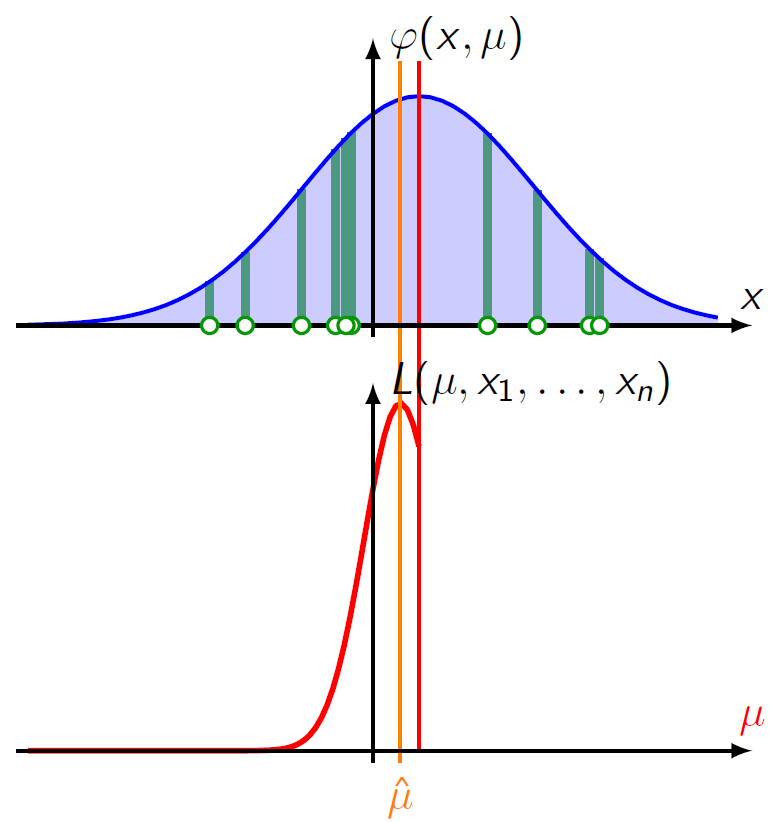
\includegraphics[width=\columnwidth]{images/likelihood.png} 
\end{minipage}
\hfill
\begin{minipage}{0.5\columnwidth}
    Bewerte Kandidaten $\crd{\mu}$ mit der Likelihood-Funktion 

    $$ L(\mu, x_1, ... x_n) = \cgn{\varphi(x_1, \mu)} \, ... \,  \cgn{\varphi(x_n, \mu)} $$
    $$ \text{ \textrightarrow\ } \cor{\hat{\mu}} = \mathrm{arg \, max}_{\substack{\mu}} L(\mu, x_1, ... x_n) $$
\end{minipage}

\vspace{0.2cm}

\myul{\textbf{Likelihood-Funktion}}
$$ L(\vartheta, x_1, ... x_n) = \varphi(\vartheta, x_1) \cdot \varphi(\vartheta, x_2) ... \varphi(\vartheta, x_n) $$
Wahrscheinlichkeit für die Werte $x_i$ 

\vspace{0.2cm}

\myul{\textbf{Prinzip}}
\vspace{0.1cm}

$\hat{\vartheta}(x_1, ..., x_n)$ maximiert  $L(\vartheta, x_1, ... x_n)$ (Maximum-Likelihood-Schätzer) \\
\textrightarrow\ Ableiten und Null setzen!


\example{Schätzung von $\bm{\mu}$}

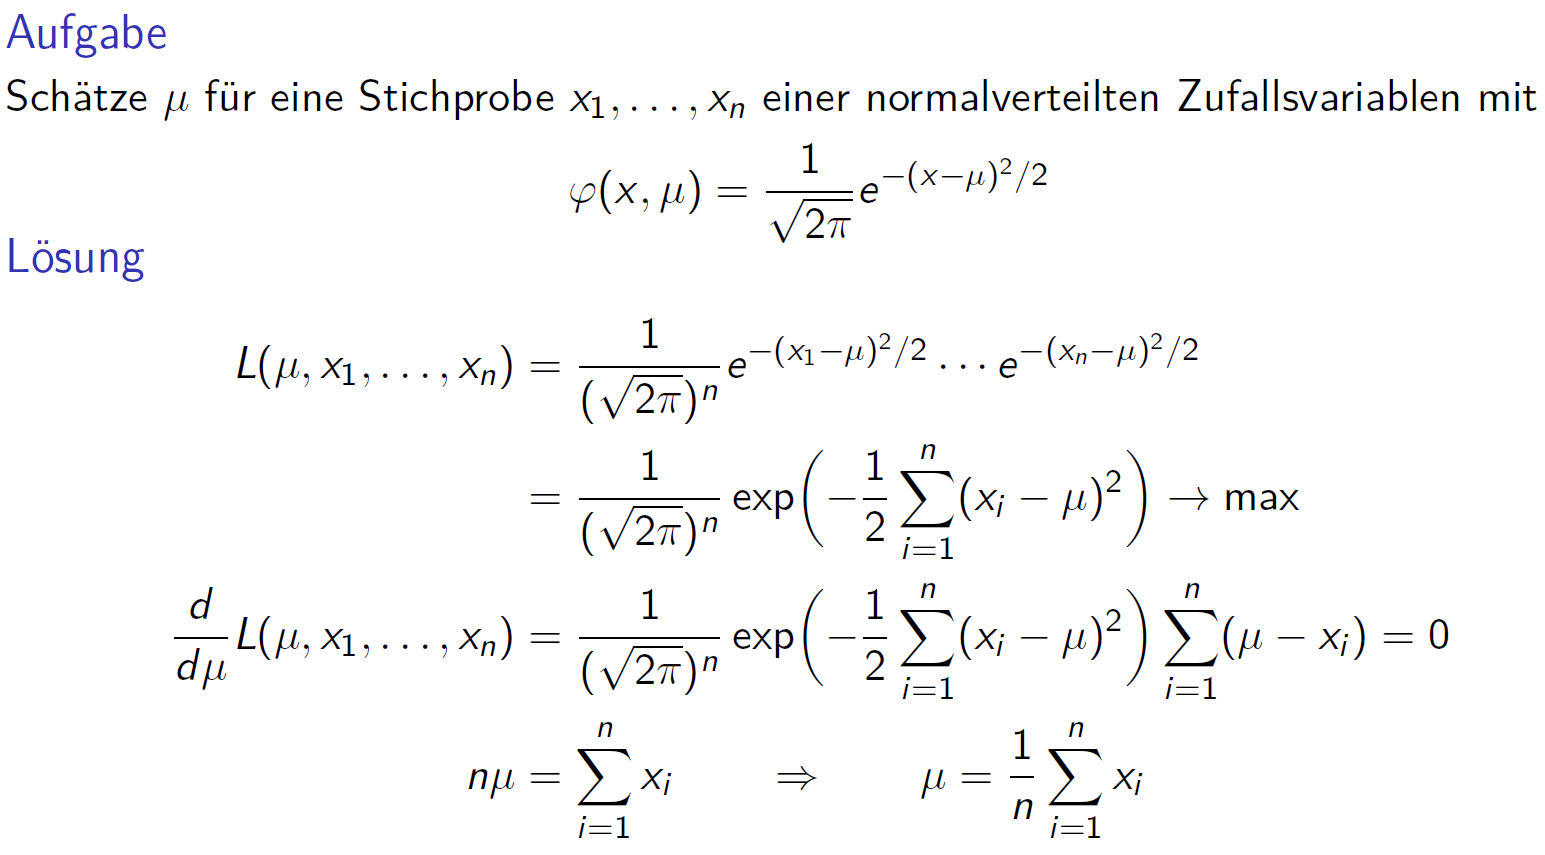
\includegraphics[width=\columnwidth]{images/likelihood_beispiel.png}


\subsection{Konfidenzintervall}

 $[\vartheta_-, \vartheta_+]$ heisst \textbf{Konfidenzintervall} zum (Vertrauens-)Niveau $1 - \alpha$ 

\vspace{0.2cm}

\myul{\textbf{Aufgabe:}}

\vspace{0.1cm}

Finde ein Intervall $[\vartheta_-, \vartheta_+]$, das den wahren Wert des Parameters mit Wahrscheinlichkeit $1 - \alpha$ enthält.

\vspace{0.2cm}

\begin{minipage}{0.4\columnwidth}
    \includegraphics[width=\columnwidth]{images/Konfidenzintervall}
\end{minipage}
\hfill
\begin{minipage}{0.55\columnwidth}
    \myul{\textbf{Lösung}}

    \vspace{0.1cm}

    \begin{itemize}
        \item  Verteilung von $\vartheta$: \\
            Wahrscheinlichtsichte $\varphi(\vartheta)$ und Verteilungsfunktion $F_{\vartheta}$
        \item Finde $\vartheta$-Werte so, dass $1 - \alpha = F(\vartheta_+) - F(\vartheta_-)$
    \end{itemize}
\end{minipage}


\subsection{Intervallschätzung}

\myul{\textbf{Aufgabe}}

\vspace{0.1cm}

Gegeben eine normalverteilte Stichprobe $X_i$, $i = 1, \, \ldots \, n$ 
Finde ein Intervall, welches $\mu$ mit Warhscheinlichkeit 95\% enthält.
$$ \hat{\mu} = \frac{1}{n} (X_1 + \ldots + X_n) $$


\subsubsection{Lösung 1 - Bekannte Varianz}

$\hat{\mu}$ ist normalverteilt mit Erwartungswert $\mu$ und Varianz $\frac{1}{n} \sigma^2$

$$ \boxed{ \left[ \hat{\mu} - 1.96 \frac{\sigma}{\sqrt{n}} \, , \, \hat{\mu} + 1.96 \frac{\sigma}{\sqrt{n}}  \right] } $$

Das angegebene Intervall enthält $\mu$ mit Wahrscheinlichkeit 95\%


\subsubsection{Lösung 2 - Geschätzte Varianz}

$$ \boxed{ t = \frac{\hat{\mu} - \mu}{\hat{\sigma} / \sqrt{n}} \quad \text{t-verteilt mit } k = n-1 \text{ Freiheitsgraden} } $$

Finde ein Intervall $[t_- \, , \, t_+]$, das $t$ mit Wahrscheinlichkeit 95\% ethält. \\ 
Dann ist das gesuchte Intervall:

$$ \boxed{ \left[ \hat{\mu} + t_- \frac{\hat{\sigma}}{\sqrt{n}} \, , \, \hat{\mu} + t_+ \frac{\hat{\sigma}}{\sqrt{n}}  \right] } $$

\textbf{ \textrightarrow\ $\bm{t}$-Tabelle siehe Abschnitt \ref{Quantilen der t-Verteilung}}

		\section{Hypothesentests}

\subsection{Rationale Erklärungen}

\subsubsection{Was ist wahr?}

Wahr ist, was mit der objektiven Realität übereinstimmt


\subsubsection{Rationale Erklärung}

\begin{enumerate}
	\item Erklärungen müssen falsifizierbar sein
	\item Erklärungen müssen mit allen Beobachtungen übereinstimmen
\end{enumerate}


\subsection{Grundätzliche Testmethode}

\begin{minipage}{0.35\columnwidth}
	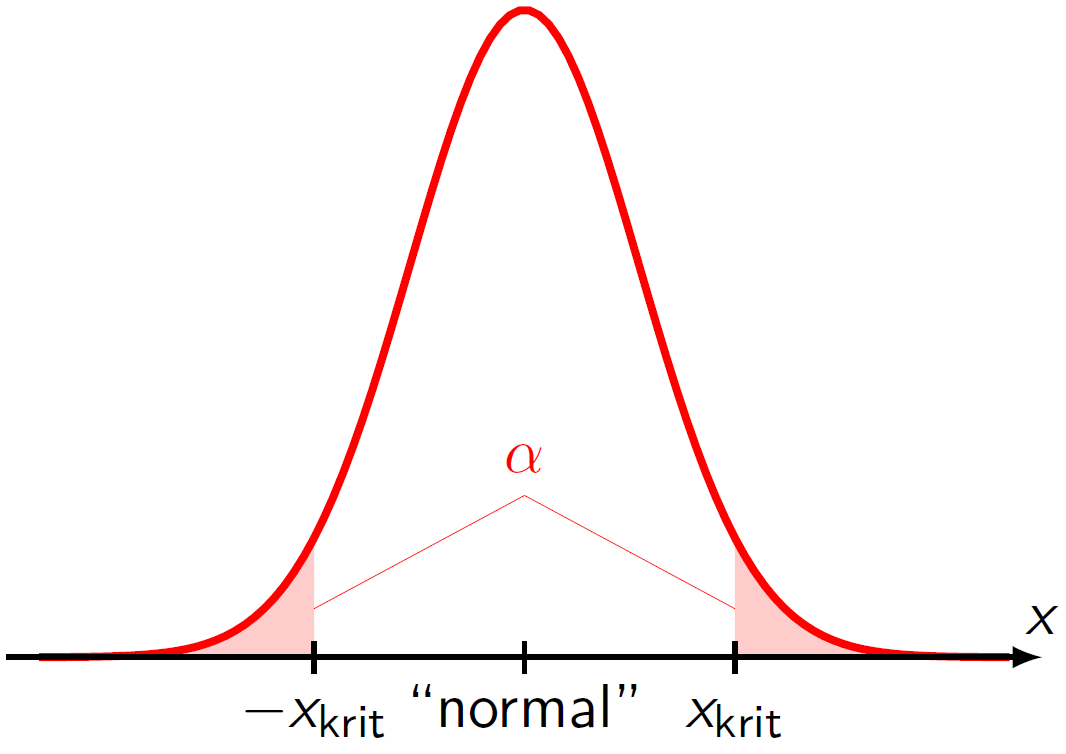
\includegraphics[width=\columnwidth]{images/vorgehen_hypothesentest.png}
\end{minipage}
\hfill
\begin{minipage}{0.6\columnwidth}
	\begin{enumerate}
		\item Nullhypothese $H_0$ formulieren 
		\item Messgrösse bestimmen, mit der $H_0$ getestet werden kann (Teststatistik)
		\item Verteilung der Messgrösse ermitteln
		\item Parameter der Verteilung schätzen
		\item Kritischen Wert für die Testgrösse bestimmen, der nur mit Wahrscheinlichkeit  $\alpha$ überschritten wird.
		\item Ist die Messgrösse im vorliegenden Experiment 'unwahrscheinlich gross? \\
			\textrightarrow\ $H_0$ verwerfen
	\end{enumerate}
\end{minipage}


\subsection{Vorgehen Hypothesentest}

\begin{tabular}{ll}
	$H_0$	& Nullhypothese 'nichts besonderes' (zu widerlegen!)							\\
	$H_1$ 	& Alternativhypothese \textrightarrow\ \textbf{Genau das Gegenteil} von $H_0$
\end{tabular}


\subsubsection{Vorgehen (!)}

\begin{enumerate}
	\item Nullhypothese $H_0$ und Alternativhypothese $H_1$ 
	\item Testgrösse und Verteilung (Testmethode) unter der Annahme der Nullhypothese $H_0$ \\
		\textrightarrow\ Testmethode wählen gemäss Abschnitt \ref{Wahl der richtigen Testmethode}
	\item Wahl des Signifikanzniveaus $\alpha$
	\item Kritischer Wert für Testgrösse, die nur mit Wahrscheinlichkeit $\alpha$ erreicht wird 
	\item Testgrösse $>$ kritischer Wert \textrightarrow\ Nullhypothese $H_0$ \textbf{verwerfen}
\end{enumerate}


\subsubsection{Einschränkungen}

\begin{itemize}
	\item Alternative muss die Negation der Nullhypothese sein \\
		(Fehschluss des falschen Dilemmas)
	\item Es kann viele Möglichkeiten der Widerlegung der Nullhypothese geben
	\item Wenn ein Test scheitert, heisst das nicht, dass die Nullhypothese wahr ist, sondern nur, dass sie noch nicht widerlegt werden konnte 
\end{itemize}


\subsection{Fehlerarten}

\myul{\textbf{Fehler 1. Art}}

\vspace{0.1cm}

Nullhypothese verworfen, obwohl wahr (zufallsbedingt unwahrscheinlicher Wert der Teststatistik, falsch positives Ergebnis) \\
\textbf{\textrightarrow\ Fehler 1. Art tritt mit Wahrscheinlichkeit $\bm{\alpha}$ auf}

\vspace{0.2cm}

\myul{\textbf{Fehler 2. Art}}

\vspace{0.1cm}

Nullhypothese nicht verworfen, obwohl falsch (falsch negatives Ergebnis)

\vspace{0.2cm}


\subsubsection{Typische Werte für $\bm{\alpha}$ }

\begin{center}
	\begin{tabular}{l | l}
		$\alpha$ 		& 							\\
		\hline
		$\bm{0.05}$		& \textbf{'signifikant'} 	\\
		\hline
		$0.01$ 			& 'hoch signifikant' 		\\
		$0.001$ 		& 'hoch signifikant' 		\\
		\hline
	\end{tabular}
\end{center}


\example{Hypothesentest: Faire Münze}

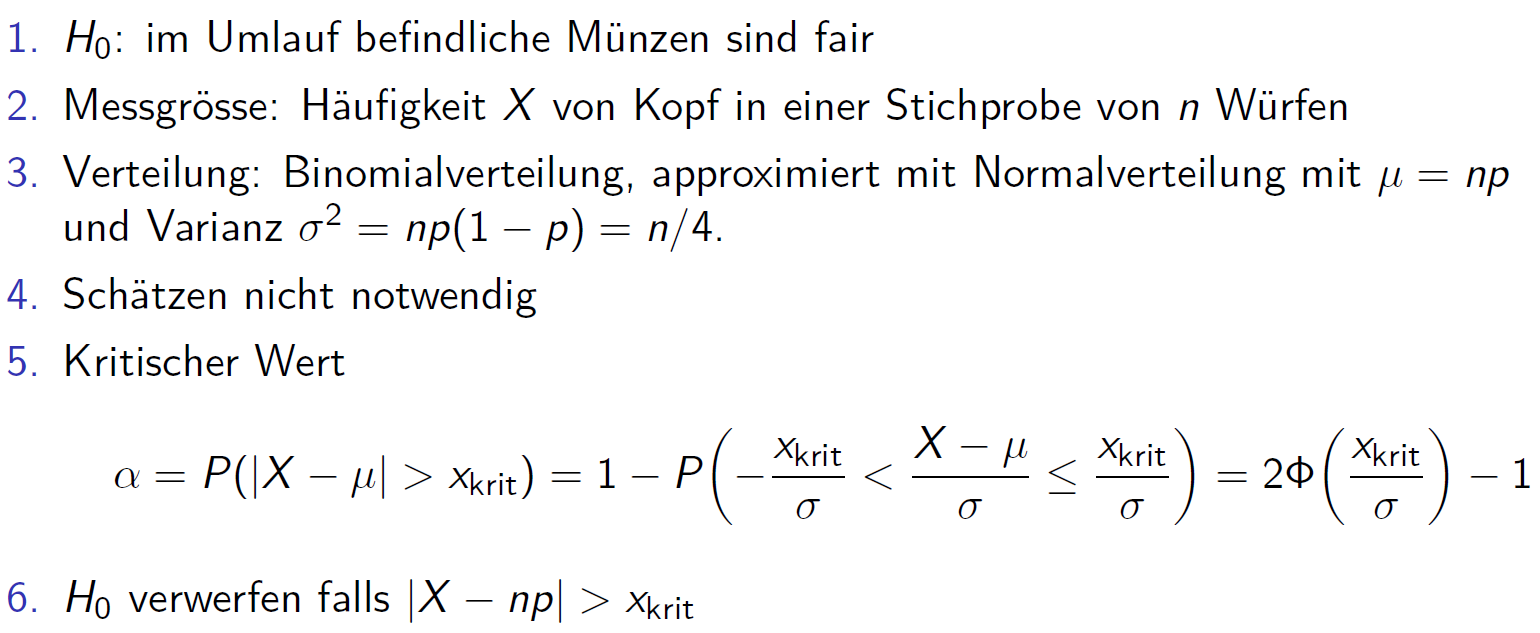
\includegraphics[width=\columnwidth]{images/beispiel_faire_muenze.png}


\subsection{Wahl der richtigen Testmethode}
\label{Wahl der richtigen Testmethode}

\begin{itemize}
	\setlength\itemsep{5pt}
	\item Wahrscheinlichkeiten (diskrete Verteilung mit endlicher Anzahl Versuchsausgänge) prüfen \\
 		\textrightarrow\ $\chi^2$-Test 
 
 	\item Prüfen auf (gleichen) Erwartungswert $E(X)$ \\
	 \textrightarrow\ $t$-Test 
 
 	\item Abweichung von Mittelwert prüfen \\
 		\textrightarrow\ Normalverteilung 
 
 	\item Prüfung auf Abweichung von Verteilungsfunktion $F(x)$ \\
		\textrightarrow\ Kolmogorov-Smirnov-Test 
\end{itemize}


\subsection[Hypothesentest mit t-Verteilung]{Hypothesentest mit $t$-Verteilung}

\subsubsection{Nullhypothese $\bm{H_0}$}

Die Stichproben $X_1,\, \ldots , \, X_n \text{ und } Y_1, \, \ldots , \, Y_m$ mit gleicher Varianz haben den gleichen Erwartungswert. 


\subsubsection{Teststatistik}

$$ t = \frac{\overline{X} - \overline{Y}}{\sqrt{(n-1) S_X^2 + (m-1) S_Y^2}} \, \sqrt{\frac{n \, m \, (n+m-2)}{n+m}} $$

ist $t$-verteilt mit $k = m+n-2$ Freiheitsgraden


\subsubsection{Parameter schätzen}

\begin{minipage}[c]{0.48\columnwidth}
	$$ \overline{X} = \frac{X_1 + \ldots + X_n}{n} $$
\end{minipage}
\hfill
\begin{minipage}[c]{0.48\columnwidth}
	$$ S_X^2 = \frac{1}{n-1} \sum\limits_{i=1}^n (X_i - \overline{X})^2 $$
\end{minipage}

\vspace{0.2cm}

\begin{minipage}[c]{0.48\columnwidth}
	$$ \overline{Y} = \frac{Y_1+ \ldots + Y_m}{m} $$
\end{minipage}
\hfill
\begin{minipage}[c]{0.48\columnwidth}
	$$ S_Y^2 = \frac{1}{m-1} \sum\limits_{i=1}^m (Y_i - \overline{Y})^2 $$
\end{minipage}

\vspace{0.2cm}

\textrightarrow\ Tabelle $t$-Verteilung siehe Abschnitt \ref{Quantilen der t-Verteilung}


\subsection[p-Value]{$p$-Value}

\begin{minipage}[c]{0.35\columnwidth}
	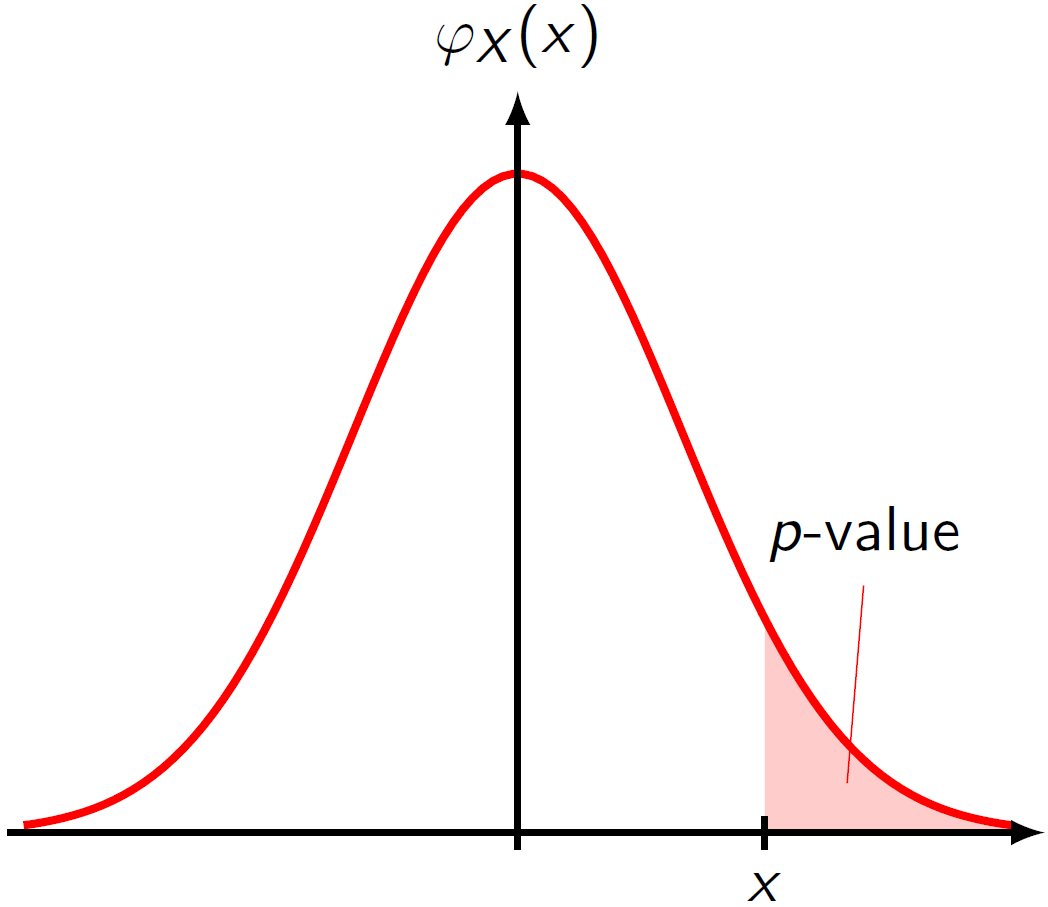
\includegraphics[width=\columnwidth]{images/p-value.png}
\end{minipage}
\hfill
\begin{minipage}[c]{0.58\columnwidth}
	Der $p$-Value beschreibt die \textbf{Wahrscheinlichkeit, einen Wert $> x$} zu erhalten
	$$ \boxed{ p-\text{Value} = \alpha = P(X > x) = 1 - F(x) } $$

	\myul{\textbf{Interpretation}}

	\vspace{0.1cm}

	$p$-Values beschreiben Wahrscheinlichkeit für Fehler 1. Art
\end{minipage}


\subsection[x2-Test]{$\chi^2$-Test}

Testen einer \textbf{diskreten} Verteilung \\
\textbf{Mehrere Versuchsausgänge} (endliche Anzahl) möglich! 

\vspace{0.2cm}

Diskrete Verteilung $P(X = x_i) = p_i$ mit $n_i$ Beobachtungen für jeden Wert

\vspace{0.2cm}

\begin{enumerate}
	\item $H_0$: Beobachtete Häufigkeiten $n_i$ entsprechen Wahrscheinlichkeiten $p_i$ 
	\item Messgrösse: Diskrepanz $D$
	\item Verteilung: $\chi^2$-Verteilung mit $k = d-1$ Freiheitsgraden \\
		$d = $ Anzahl mögliche Versuchsausgänge
	\item Signifikanzniveau $\alpha$ wählen
	\item Schätzen: nicht nötig
	\item Kritischer Wert: $D_{\rm krit}$ aus der $\chi^2$-Tabelle (Abschnitt \ref{Quantilen der chi2-Verteilung})
	\item $H_0$ verwerfen wenn $D > D_{\rm krit}$
\end{enumerate}

\vspace{0.2cm}

\textbf{Einschränkung:} $n_i \geq 5$ (zentraler Grenzwertsatz)


\subsubsection{Messgrösse: Diskrepanz $D$}

$$ \boxed{ D = \sum\limits_{i = 1}^d \frac{(n_i - n \, p_i)^2}{n \, p_i}} $$

\begin{tabular}{ll}
	$n$ 	& Totale Anzahl Versuche 								\\
	$n_i$ 	& Wie oft Ergebnis $i$ eingetreten ist 					\\
	$p_i$ 	& Wahrscheinlichkeit $P(X = x_i)$ gemäss Nullhypothese 
\end{tabular}


\subsection{Kolmogorov-Smirnov-Test}

\textbf{Frage: } 'Folgt eine Zufallsvariable einer gegebenen Verteilung?' \\
\textbf{\textrightarrow\ Daten $\bm{x_i}$ müssen zuerst \myul{aufsteigend} sortiert werden!}

\vspace{0.2cm}

\begin{minipage}{0.4\columnwidth}
	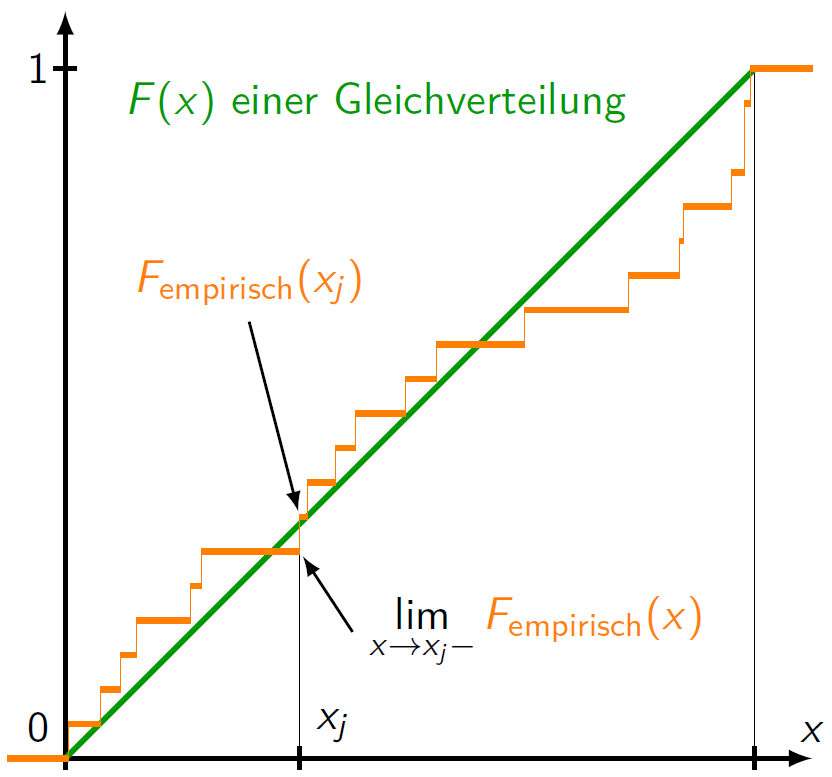
\includegraphics[width=\columnwidth]{images/empirische_verteilungsfunktion.png}
\end{minipage}
\hfill
\begin{minipage}{0.58\columnwidth}
	Daten: $x_1 \leq \ldots \leq x_j \leq \ldots \leq x_n$ 

	$$ \boxed{ \cor{F_{\text{empirisch}}(x_j)} = \frac{j}{n} } $$
	$$ \boxed{ \lim\limits_{x \to \_j^-} \cor{F_{\text{empirisch}}(x_j)} = \frac{j-1}{n} } $$
\end{minipage}

\vspace{0.2cm}

Abweichung der \cor{empirischen Verteilungsfunktion} von der \cgn{Verteilungsfunktion}: 

$$ \boxed{ K_n^+ = \sqrt{n} \, \mathrm{max}_x(F_{\text{empirisch}}(x) - F(x)) = \sqrt{n} \, \mathrm{max}_j \Big( \frac{j}{n} - F(x_j) \Big)  } $$
$$ \boxed{ K_n^- = \sqrt{n} \, \mathrm{max}_x( F(x) - F_{\text{empirisch}}(x)) = \sqrt{n} \, \mathrm{max}_j \Big( F(x_j) - \frac{j-1}{n} \Big)  } $$

\vspace{0.2cm}

\textrightarrow\ Falls $K_n^+ > K_{\rm krit}$ \textrightarrow\ $H_0$ verwerfen \\
\textrightarrow\ KS-Tabelle siehe Abschnitt \ref{Quantilen für Kolmogorov-Smirnov-Test}


\subsection{Q-Q-Plot}

\textbf{Frage:} 'Gehören zwei Datensätze zur gleichen Verteilung?'

\vspace{0.2cm}

\begin{minipage}{0.3\columnwidth}
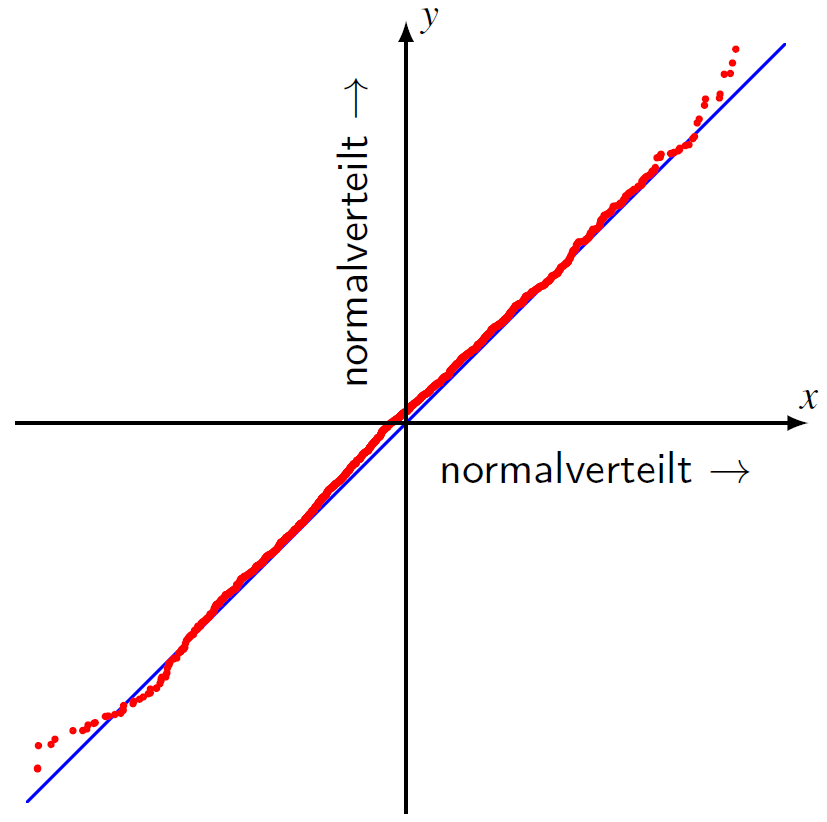
\includegraphics[width=\columnwidth]{images/Q-Q-plot.png}
\end{minipage}
\hfill
\begin{minipage}{0.6\columnwidth}
	\myul{\textbf{Verteilungsvergleich}}

	\vspace{0.2cm}

	\begin{enumerate}
		\setlength\itemsep{5pt}
		\item  \textbf{sortieren} \\
			$x_1 \leq ... \leq ... \leq x_n$ \\
			$y_1 \leq ... \leq ... \leq y_n$ 
		\item Punkte $p_i = (x_i, y_i)$ darstellen 
		\item Gleiche Verteilung, wenn Punkte $P_i$ ungefähr auf einer \textbf{Geraden} liegen 
	\end{enumerate}
\end{minipage}


		\section{Filtern}

'Filtern' bedeutet, einen \textbf{optimalen Schätzer} zu finden


\subsection{Optimale Schätzung}

$X_1$ und $X_2$ sind  unabhängige Messungen von $\mu$ mit Messfehler $\var(X_i) = \sigma_i^2 $ 


\subsubsection{Ansatz}

Linearkombination 
$$ \boxed{ X = t \, X_1 + (1-t) \, X_2} $$
so wählen, dass $\var(X)$ minimal wird \\
\textrightarrow\ $X$ entspricht dem 'gewichteten Mittelwert' der Messungen


\subsubsection{Parameter}

\begin{minipage}{0.48\columnwidth}
    $$ \boxed{ t = \frac{\sigma_2^2}{\sigma_1^2 + \sigma_2^2} }$$
\end{minipage}
\hfill
\begin{minipage}{0.48\columnwidth}
    $$ \boxed{ 1-t  = \frac{\sigma_1^2}{\sigma_1^2 + \sigma_2^2} }$$
\end{minipage}


\subsubsection{Lösung}

\begin{minipage}{0.6\columnwidth}
    $$ \boxed{ X = \underbrace{ \frac{\sigma_2^2}{\sigma_1^2 + \sigma_2^2} }_{\substack{t}}  \, X_1 +  
    \underbrace{ \frac{\sigma_1^2}{\sigma_1^2 + \sigma_2^2} }_{\substack{(1-t)}} \, X_2 } $$
\end{minipage}
\hfill
\begin{minipage}{0.38\columnwidth}
    $$ \boxed{ \var(X) = \frac{\sigma_1^2 \, \sigma_2^2}{\sigma_1^2 + \sigma_2^2} } $$
\end{minipage}


		\section{Anhang}

\subsubsection{Wie löst man WrStat Übungen?}

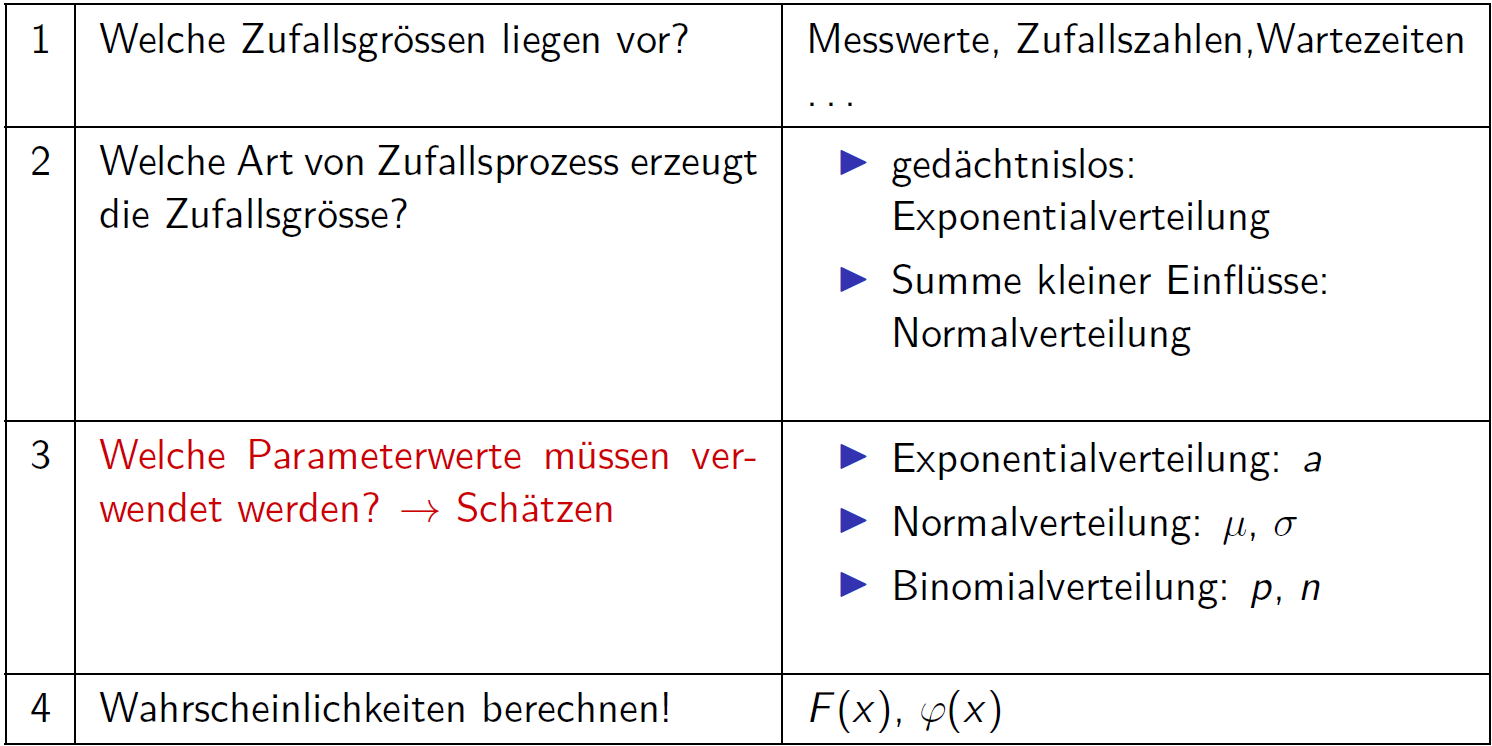
\includegraphics[width=\columnwidth]{images/wrstat_uebungen_loesen.png}


    \end{layout}

	% % Quelle: LaTeX Code aus Skirip von A. Müller 
% % (modifiziert)

\section{Tabellen}

\subsection{Verteilungsfunktion der Normalverteilung}
\label{Verteilungsfunktion der Normalverteilung}


\begin{center}
    \small
    \begin{tabular}{|r|rrrrrrrrrr|}
        \hline
        $x$&+0.00&+0.01&+0.02&+0.03&+0.04&+0.05&+0.06&+0.07&+0.08&+0.09\\
        \hline
        0.0&0.5000&0.5040&0.5080&0.5120&0.5160&0.5199&0.5239&0.5279&0.5319&0.5359\\
        0.1&0.5398&0.5438&0.5478&0.5517&0.5557&0.5596&0.5636&0.5675&0.5714&0.5753\\
        0.2&0.5793&0.5832&0.5871&0.5910&0.5948&0.5987&0.6026&0.6064&0.6103&0.6141\\
        0.3&0.6179&0.6217&0.6255&0.6293&0.6331&0.6368&0.6406&0.6443&0.6480&0.6517\\
        0.4&0.6554&0.6591&0.6628&0.6664&0.6700&0.6736&0.6772&0.6808&0.6844&0.6879\\
        0.5&0.6915&0.6950&0.6985&0.7019&0.7054&0.7088&0.7123&0.7157&0.7190&0.7224\\
        0.6&0.7257&0.7291&0.7324&0.7357&0.7389&0.7422&0.7454&0.7486&0.7517&0.7549\\
        0.7&0.7580&0.7611&0.7642&0.7673&0.7704&0.7734&0.7764&0.7794&0.7823&0.7852\\
        0.8&0.7881&0.7910&0.7939&0.7967&0.7995&0.8023&0.8051&0.8078&0.8106&0.8133\\
        0.9&0.8159&0.8186&0.8212&0.8238&0.8264&0.8289&0.8315&0.8340&0.8365&0.8389\\
        1.0&0.8413&0.8438&0.8461&0.8485&0.8508&0.8531&0.8554&0.8577&0.8599&0.8621\\
        1.1&0.8643&0.8665&0.8686&0.8708&0.8729&0.8749&0.8770&0.8790&0.8810&0.8830\\
        1.2&0.8849&0.8869&0.8888&0.8907&0.8925&0.8944&0.8962&0.8980&0.8997&0.9015\\
        1.3&0.9032&0.9049&0.9066&0.9082&0.9099&0.9115&0.9131&0.9147&0.9162&0.9177\\
        1.4&0.9192&0.9207&0.9222&0.9236&0.9251&0.9265&0.9279&0.9292&0.9306&0.9319\\
        1.5&0.9332&0.9345&0.9357&0.9370&0.9382&0.9394&0.9406&0.9418&0.9429&0.9441\\
        1.6&0.9452&0.9463&0.9474&0.9484&0.9495&0.9505&0.9515&0.9525&0.9535&0.9545\\
        1.7&0.9554&0.9564&0.9573&0.9582&0.9591&0.9599&0.9608&0.9616&0.9625&0.9633\\
        1.8&0.9641&0.9649&0.9656&0.9664&0.9671&0.9678&0.9686&0.9693&0.9699&0.9706\\
        1.9&0.9713&0.9719&0.9726&0.9732&0.9738&0.9744&0.9750&0.9756&0.9761&0.9767\\
        2.0&0.9772&0.9778&0.9783&0.9788&0.9793&0.9798&0.9803&0.9808&0.9812&0.9817\\
        2.1&0.9821&0.9826&0.9830&0.9834&0.9838&0.9842&0.9846&0.9850&0.9854&0.9857\\
        2.2&0.9861&0.9864&0.9868&0.9871&0.9875&0.9878&0.9881&0.9884&0.9887&0.9890\\
        2.3&0.9893&0.9896&0.9898&0.9901&0.9904&0.9906&0.9909&0.9911&0.9913&0.9916\\
        2.4&0.9918&0.9920&0.9922&0.9925&0.9927&0.9929&0.9931&0.9932&0.9934&0.9936\\
        2.5&0.9938&0.9940&0.9941&0.9943&0.9945&0.9946&0.9948&0.9949&0.9951&0.9952\\
        2.6&0.9953&0.9955&0.9956&0.9957&0.9959&0.9960&0.9961&0.9962&0.9963&0.9964\\
        2.7&0.9965&0.9966&0.9967&0.9968&0.9969&0.9970&0.9971&0.9972&0.9973&0.9974\\
        2.8&0.9974&0.9975&0.9976&0.9977&0.9977&0.9978&0.9979&0.9979&0.9980&0.9981\\
        2.9&0.9981&0.9982&0.9982&0.9983&0.9984&0.9984&0.9985&0.9985&0.9986&0.9986\\
        3.0&0.9987&0.9987&0.9987&0.9988&0.9988&0.9989&0.9989&0.9989&0.9990&0.9990\\
        \hline
    \end{tabular}
\end{center}


\subsection{Quantilen für Kolmogorov-Smirnov-Test}
\label{Quantilen für Kolmogorov-Smirnov-Test}
    
\begin{center}
    \small
    \begin{tabular}{|r|rrr|rrr|rrr|}
        \hline
        $n$&$p=0.01$&$p=0.05$&$p=0.1$&$p=0.25$&$p=0.5$&$p=0.75$&$p=0.9$&$p=0.95$&$p=0.99$\\
        \hline
        1&0.01000&0.05000&0.10000&0.25000&0.50000&0.75000&0.90000&0.95000&0.99000\\
        2&0.01400&0.06749&0.12955&0.29289&0.51764&0.70711&0.96700&1.09799&1.27279\\
        3&0.01699&0.07919&0.14714&0.31117&0.51469&0.75394&0.97828&1.10166&1.35889\\
        4&0.01943&0.08789&0.15899&0.32023&0.51104&0.76419&0.98531&1.13043&1.37774\\
        5&0.02152&0.09471&0.16750&0.32490&0.52449&0.76741&0.99948&1.13916&1.40242\\
        6&0.02336&0.10022&0.17385&0.32717&0.53193&0.77028&1.00520&1.14634&1.41435\\
        7&0.02501&0.10479&0.17873&0.32804&0.53635&0.77552&1.00929&1.15373&1.42457\\
        8&0.02650&0.10863&0.18256&0.32802&0.53916&0.77971&1.01346&1.15859&1.43272\\
        9&0.02786&0.11191&0.18560&0.32745&0.54109&0.78246&1.01731&1.16239&1.43878\\
        10&0.02912&0.11473&0.18803&0.32975&0.54258&0.78454&1.02016&1.16582&1.44397\\
        11&0.03028&0.11718&0.19000&0.33304&0.54390&0.78633&1.02249&1.16885&1.44837\\
        12&0.03137&0.11933&0.19160&0.33570&0.54527&0.78802&1.02458&1.17139&1.45207\\
        13&0.03239&0.12123&0.19291&0.33789&0.54682&0.78966&1.02649&1.17357&1.45527\\
        14&0.03334&0.12290&0.19396&0.33970&0.54856&0.79122&1.02823&1.17552&1.45810\\
        15&0.03424&0.12439&0.19482&0.34122&0.55002&0.79259&1.02977&1.17728&1.46060\\
        16&0.03509&0.12573&0.19552&0.34250&0.55123&0.79377&1.03113&1.17888&1.46283\\
        17&0.03589&0.12692&0.19607&0.34360&0.55228&0.79482&1.03237&1.18032&1.46483\\
        18&0.03665&0.12799&0.19650&0.34454&0.55319&0.79578&1.03351&1.18162&1.46664\\
        19&0.03738&0.12895&0.19684&0.34535&0.55400&0.79667&1.03457&1.18282&1.46830\\
        20&0.03807&0.12982&0.19709&0.34607&0.55475&0.79752&1.03555&1.18392&1.46981\\
        30&0.04354&0.13510&0.20063&0.35087&0.56047&0.80362&1.04243&1.19164&1.48009\\
        50&0.05005&0.13755&0.20794&0.35713&0.56644&0.80988&1.04933&1.19921&1.48969\\
        100&0.05698&0.14472&0.21370&0.36331&0.57269&0.81634&1.05627&1.20666&1.49864\\
        200&0.06049&0.14887&0.21816&0.36784&0.57725&0.82099&1.06117&1.21180&1.50458\\
        \hline
    \end{tabular}
\end{center}

\vfill\null
\pagebreak

\subsection[Quantilen der chi2-Verteilung]{Quantilen der $\chi^2$-Verteilung}
\label{Quantilen der chi2-Verteilung}

\vspace{-0.2cm}
$$ \boxed{ p = 1 - \alpha} \qquad \qquad \boxed{ k = \text{Anzahl Versuchsausgänge } -1 } $$

\begin{center}
    \small
    \begin{tabular}{|r|rrr|rrr|rrr|}
        \hline
        \strut$k$&$p=0.01$&$p=0.05$&$p=0.1$&$p=0.25$&$p=0.5$&$p=0.75$&$p=0.9$&$p=0.95$&$p=0.99$\\
        \hline
        1&0.000&0.004&0.016&0.102&0.455&1.323&2.706&3.841&6.635\\
        2&0.020&0.103&0.211&0.575&1.386&2.773&4.605&5.991&9.210\\
        3&0.115&0.352&0.584&1.213&2.366&4.108&6.251&7.815&11.345\\
        4&0.297&0.711&1.064&1.923&3.357&5.385&7.779&9.488&13.277\\
        5&0.554&1.145&1.610&2.675&4.351&6.626&9.236&11.070&15.086\\
        6&0.872&1.635&2.204&3.455&5.348&7.841&10.645&12.592&16.812\\
        7&1.239&2.167&2.833&4.255&6.346&9.037&12.017&14.067&18.475\\
        8&1.646&2.733&3.490&5.071&7.344&10.219&13.362&15.507&20.090\\
        9&2.088&3.325&4.168&5.899&8.343&11.389&14.684&16.919&21.666\\
        10&2.558&3.940&4.865&6.737&9.342&12.549&15.987&18.307&23.209\\
        11&3.053&4.575&5.578&7.584&10.341&13.701&17.275&19.675&24.725\\
        12&3.571&5.226&6.304&8.438&11.340&14.845&18.549&21.026&26.217\\
        13&4.107&5.892&7.042&9.299&12.340&15.984&19.812&22.362&27.688\\
        14&4.660&6.571&7.790&10.165&13.339&17.117&21.064&23.685&29.141\\
        15&5.229&7.261&8.547&11.037&14.339&18.245&22.307&24.996&30.578\\
        16&5.812&7.962&9.312&11.912&15.338&19.369&23.542&26.296&32.000\\
        17&6.408&8.672&10.085&12.792&16.338&20.489&24.769&27.587&33.409\\
        18&7.015&9.390&10.865&13.675&17.338&21.605&25.989&28.869&34.805\\
        19&7.633&10.117&11.651&14.562&18.338&22.718&27.204&30.144&36.191\\
        20&8.260&10.851&12.443&15.452&19.337&23.828&28.412&31.410&37.566\\
        21&8.897&11.591&13.240&16.344&20.337&24.935&29.615&32.671&38.932\\
        22&9.542&12.338&14.041&17.240&21.337&26.039&30.813&33.924&40.289\\
        23&10.196&13.091&14.848&18.137&22.337&27.141&32.007&35.172&41.638\\
        24&10.856&13.848&15.659&19.037&23.337&28.241&33.196&36.415&42.980\\
        25&11.524&14.611&16.473&19.939&24.337&29.339&34.382&37.652&44.314\\
        26&12.198&15.379&17.292&20.843&25.336&30.435&35.563&38.885&45.642\\
        27&12.879&16.151&18.114&21.749&26.336&31.528&36.741&40.113&46.963\\
        28&13.565&16.928&18.939&22.657&27.336&32.620&37.916&41.337&48.278\\
        29&14.256&17.708&19.768&23.567&28.336&33.711&39.087&42.557&49.588\\
        30&14.953&18.493&20.599&24.478&29.336&34.800&40.256&43.773&50.892\\
        50&29.707&34.764&37.689&42.942&49.335&56.334&63.167&67.505&76.154\\
        100&70.065&77.929&82.358&90.133&99.334&109.141&118.498&124.342&135.807\\
        500&429.388&449.147&459.926&478.323&499.333&520.950&540.930&553.127&576.493\\
        1000&898.912&927.594&943.133&969.484&999.333&1029.790&1057.724&1074.679&1106.969\\
        \hline
    \end{tabular}
\end{center}


 
\subsection{Quantilen der t-Verteilung}
\label{Quantilen der t-Verteilung}

\vspace{-0.2cm}
$$ \boxed{ p = 1 - \alpha} \qquad \qquad \boxed{ k = m + n - 2 \text{ Freiheitsgrade} } $$

\begin{center}
    \small
    \begin{tabular}{|r|rrrrrrr|}
        \hline
        $k$&0.75&0.8&0.9&0.95&0.975&0.99&0.995\\
        \hline
        1&1.0000&1.3764&3.0777&6.3138&12.7062&31.8205&63.6567\\
        2&0.8165&1.0607&1.8856&2.9200&4.3027&6.9646&9.9248\\
        3&0.7649&0.9785&1.6377&2.3534&3.1824&4.5407&5.8409\\
        4&0.7407&0.9410&1.5332&2.1318&2.7764&3.7469&4.6041\\
        5&0.7267&0.9195&1.4759&2.0150&2.5706&3.3649&4.0321\\
        6&0.7176&0.9057&1.4398&1.9432&2.4469&3.1427&3.7074\\
        7&0.7111&0.8960&1.4149&1.8946&2.3646&2.9980&3.4995\\%
        8&0.7064&0.8889&1.3968&1.8595&2.3060&2.8965&3.3554\\
        9&0.7027&0.8834&1.3830&1.8331&2.2622&2.8214&3.2498\\
        10&0.6998&0.8791&1.3722&1.8125&2.2281&2.7638&3.1693\\
        11&0.6974&0.8755&1.3634&1.7959&2.2010&2.7181&3.1058\\
        12&0.6955&0.8726&1.3562&1.7823&2.1788&2.6810&3.0545\\
        13&0.6938&0.8702&1.3502&1.7709&2.1604&2.6503&3.0123\\
        14&0.6924&0.8681&1.3450&1.7613&2.1448&2.6245&2.9768\\
        15&0.6912&0.8662&1.3406&1.7531&2.1314&2.6025&2.9467\\
        16&0.6901&0.8647&1.3368&1.7459&2.1199&2.5835&2.9208\\
        17&0.6892&0.8633&1.3334&1.7396&2.1098&2.5669&2.8982\\
        18&0.6884&0.8620&1.3304&1.7341&2.1009&2.5524&2.8784\\
        19&0.6876&0.8610&1.3277&1.7291&2.0930&2.5395&2.8609\\
        20&0.6870&0.8600&1.3253&1.7247&2.0860&2.5280&2.8453\\
        21&0.6864&0.8591&1.3232&1.7207&2.0796&2.5176&2.8314\\
        22&0.6858&0.8583&1.3212&1.7171&2.0739&2.5083&2.8188\\
        23&0.6853&0.8575&1.3195&1.7139&2.0687&2.4999&2.8073\\
        24&0.6848&0.8569&1.3178&1.7109&2.0639&2.4922&2.7969\\
        25&0.6844&0.8562&1.3163&1.7081&2.0595&2.4851&2.7874\\
        26&0.6840&0.8557&1.3150&1.7056&2.0555&2.4786&2.7787\\
        27&0.6837&0.8551&1.3137&1.7033&2.0518&2.4727&2.7707\\
        28&0.6834&0.8546&1.3125&1.7011&2.0484&2.4671&2.7633\\
        29&0.6830&0.8542&1.3114&1.6991&2.0452&2.4620&2.7564\\
        30&0.6828&0.8538&1.3104&1.6973&2.0423&2.4573&2.7500\\
        50&0.6794&0.8489&1.2987&1.6759&2.0086&2.4033&2.6778\\
        100&0.6770&0.8452&1.2901&1.6602&1.9840&2.3642&2.6259\\
        500&0.6750&0.8423&1.2832&1.6479&1.9647&2.3338&2.5857\\
        $10^3$&0.6747&0.8420&1.2824&1.6464&1.9623&2.3301&2.5808\\
        $10^4$&0.6745&0.8417&1.2816&1.6450&1.9602&2.3267&2.5763\\
        $10^5$&0.6745&0.8416&1.2816&1.6449&1.9600&2.3264&2.5759\\
        $10^6$&0.6745&0.8416&1.2816&1.6449&1.9600&2.3264&2.5758\\
        \hline
        \end{tabular}
\end{center}
    
    
\end{document}
